\documentclass
[
a4paper,
english,
oneside,
openright,                    % Kap.beginn immer rechts! (fkt. nur bei report, nicht bei article)
11pt,                         % ersatzweise 12pt, wenn mehr Seiten entstehen sollen
table
]
{book}

%%%%%%%%%%%%%%%%%%%%%%%%%%%%%%%%%%%%%%%%%%%%%%%%%%%%%%%%%%%%%%%%%%%%%%%%%%%%%%
%
% Vorlage für eine Studien- oder Diplomarbeit für den Fachbereich Informatik
% der Universität Karlsruhe (TH)
%
% Autor:   Tilo Gockel
% Version: 0.920
% Datum:   12. Mai 2010
%
% Kontakt: Hochschule Aschaffenburg,
% Tilo Gockel (Dr.-Ing.), Forschungsreferat
%
% info@formbuch.de
% http://www.formbuch.de
%
% Anmerkungen
%
% 1.) article-Style, statt report-Style
%
% Soll statt des report-Styles der article-Style genutzt werden,
% so müssen chapters durch sections, sections durch subsection usw. ersetzt
% werden. Weiterhin kann ein Kapitelbeginn auf der rechten Seite dann nicht
% mehr durch openright eingestellt werden, nur noch durch jeweilige
% \cleardoublepage -Befehle (vgl. unten).
%
%
% 2.) Lizenz
%
% Das Template darf angepasst, verändert, erweitert und auch kommerziell vertrieben werden.
% Die einzige Auflage ist, dass die Quelle des Templates in den Literaturquellen genannt
% und im Text als Quelle referenziert wird. Hierzu ist dem Text ein kurzer Satz beizufügen,
% und am Ende ist die Quelle einzufügen:
% Einzufügende Textzeile (Fußnote):
% Der vorliegende Text ist auf Basis des Latex-Templates zu [1] erstellt.
% Einzufügende zugehörige Quelle:
% [1] T. \mbox{Gockel}. Form der wissenschaftlichen Ausarbeitung. Springer-Verlag, Heidelberg, 2008.
% Begleitende Materialien unter
% \url$<http://wwwiaim.ira.uka.de/form-der-wissenschaftlichen-ausarbeitung>$.
% Weiterhin ist es sinnvoll, bei der Weitergabe des Templates die Latex-Quellen und die PDF-Datei
% nicht zu trennen.
%
%
% 3.) Versionsnummern der verwendeten Programme (alles unter Windows)
%
% (im Regelfall werden neuere Versionen aber eher von Vorteil sein)
%
%     Miktex 2.8
%     http://www.miktex.org
%
%     TexnicCenter Version 1.0 Stable Release Candidate 1
%     http://www.texniccenter.org
%
%     Texaide 4.0a
%     http://www.dessci.com/en/products/texaide
%
%     Adobe Acrobat Prof. 7.0
%     http://www.adobe.com/de/
%
%     Ghostscript 8.14, Ghostview 4.6
%     http://pages.cs.wisc.edu/~ghost
%
%     MS Office 2002, 2007 ...
%     http://office.microsoft.com/de-de/default.aspx
%
%     Adobe Photoshop CS4
%     http://www.adobe.com/de/products/photoshop/family/
%
%     Gnuplot 4.2
%     http://www.gnuplot.info
%
%     PrettyPrinter a2ps
%     http://www.gnu.org/software/a2ps
%
%     Text-Ersetzungswerkzeug grep, unter Windows
%     http://gnuwin32.sourceforge.net/packages/grep.htm
%
%
%%%%%%%%%%%%%%%%%%%%%%%%%%%%%%%%%%%%%%%%%%%%%%%%%%%%%%%%%%%%%%%%%%%%%%%%%%%%%%



\usepackage[utf8]{inputenc}   % Zeichensatz, ermöglicht die direkte Eingabe von Umlauten im Editor
\usepackage[pdftex]{graphicx} % Einbindung von Grafiken (pdf, png, jpg)
\usepackage{float}            % bietet Option [H] für bombenfestes Verankern
\usepackage[english]{babel}   % Silbentrennung nach der neuen deutschen Rechtschreibung, z.B.: Sys-tem
\usepackage{amstext}          % für Klartext via \text{} in Formeln
\usepackage{amsfonts}         % für komplexere Formeln (Mengensymbole ...)
\usepackage{amssymb}          % für komplexere Formeln (Mengensymbole ...)
\usepackage{bm}               % bold math, für \bm{}
\usepackage{enumerate}        % verbessert Aufzählungen
\usepackage[bottom]{footmisc} % Fussnoten am Seitenende
\usepackage{array}            % für Tabellen: bindet tabular-Umgebung ein
%\usepackage{algorithm}        % für Algorithmen
%\usepackage{algorithmic}      % für Algorithmen
\usepackage{ntheorem}
\usepackage{theorem}
\usepackage{pdfpages}         % für die Einbindung kompletter pdf-*Seiten*
\usepackage{parskip}          % zw. Absätzen: eine knappe Leerzeile statt hängender Einzüge
\usepackage[right]{eurosym}   % Eurosymbol
%\usepackage{xcolor}           % farbiger Text
%\usepackage{colortbl}
\usepackage{xcolor}
\usepackage{tabu}
%\usepackage[hyphens]{url}     % für \url{http://www}, Option hyp erlaubt auch Umbruch nach "-"
\usepackage{makeidx}          % Package zur Indexerstellung
\usepackage{multicol}         % zur Indexerstellung in zwei Spalten
% \usepackage[numbers, square]{natbib}   % Für \setlength{\bibsep}{3mm}; square macht eckige Klammern
\usepackage{csquotes}
\usepackage[
  style=numeric,
  backref,
  backend=biber,
  defernumbers=true,
  useprefix=true,
  giveninits=true,
  maxbibnames=99, minbibnames=99,
  sorting=none
]{biblatex}
\usepackage[T1]{fontenc}
\usepackage{hyperref}
%\usepackage{tabularx}
\usepackage{caption}
\usepackage[printonlyused]{acronym}
\usepackage{listings}
\usepackage{chngcntr}

\usepackage{tikz}
\usetikzlibrary{fit}

\usepackage{settings/chapterthumb}
\usepackage{wrapfig}

\counterwithout{figure}{chapter}
\counterwithout{table}{chapter}

\captionsetup[table]{skip=10pt}

\NeedsTeXFormat{LaTeX2e}            % Unklar, gehoeren aber zusammen:
\ProvidesPackage{hyperref}          % http://janeden.net/eigene-dokumentklassen
\hypersetup{
  pdftex=false,
  colorlinks=true,
  breaklinks=true,
  linkcolor=black,
  menucolor=black,
  urlcolor=black,
  citecolor=black
}


%\usepackage[cmex10]{amsmath}  % für erw. Formeloptionen, Option [] zur Vermeidung von Type3-Fonts
%\usepackage{mathcomp}         %\tcmu \tcohm \tccelsius.. im Mathemodus, nichtkursiv; problematisch!
%\usepackage{textcomp}         % für \textdegree , \textcelsius , macht aber manchmal auch Probleme!


%\usepackage[plainpages=false, hypertexnames=false]{hyperref}
                               % hyperref statt \url geht, verträgt sich allerdings nicht mit den
                               % eingefügten / veränderten Seitenzahlen ... (die stimmen dann nicht mehr)



\definecolor{darkred}{rgb}{0.7,0.0,0.0}
\definecolor{dunkelgrau}{rgb}{0.8,0.8,0.8}
\definecolor{hellgrau}{rgb}{0.92,0.92,0.92}
\definecolor{fgcgray}{rgb}{0.4, 0.4, 0.4}
\definecolor{bgctitle}{rgb}{0.5, 0.5, 0.5}
\definecolor{fgctitle}{rgb}{0.95, 0.95, 0.95}
\definecolor{lightgreen}{RGB}{219, 249, 189}
\definecolor{lightred}{RGB}{255, 204, 203}
\definecolor{fullred}{RGB}{255, 0, 0}

\definecolor{ob_dark_gray}{HTML}{58585a}
\definecolor{ob_light_gray}{HTML}{a5a5a6}
\definecolor{ob_orange}{HTML}{ea9023}

%\definecolor{lightgray}{rgb}{.9,.9,.9}
%\definecolor{darkgray}{rgb}{.4,.4,.4}
%\definecolor{purple}{rgb}{0.65, 0.12, 0.82}
%
%\definecolor{js-keywords}{RGB}{243, 38, 77}
%\definecolor{js-strings}{RGB}{211, 214, 95}
%\definecolor{js-comments}{RGB}{117, 113, 94}

% \renewcommand{\lstlistlistingname}{Quellcodeverzeichnis}
% \renewcommand{\lstlistingname}{Quellcode}

\renewcommand{\figurename}{Fig.}
\renewcommand{\tablename}{Tab.}
\newcommand{\sectionname}{Sec.}
\newcommand{\equationname}{Eq.}
\renewcommand{\lstlistlistingname}{List of Listings}

\newcommand{\todo}[1]{{{\color{fullred}#1}}}

\lstdefinelanguage{JavaScript}{
  keywords={typeof, new, true, false, catch, function, return, null, catch, switch, var, if, in, while, do, else, case, break},
  %keywordstyle=\color{js-keywords}\bfseries,
  ndkeywords={class, export, boolean, throw, implements, import, this},
  %ndkeywordstyle=\color{darkgray}\bfseries,
  %identifierstyle=\color{black},
  sensitive=false,
  comment=[l]{//},
  morecomment=[s]{/*}{*/},
  %commentstyle=\color{js-comments}\ttfamily,
  %stringstyle=\color{js-strings}\ttfamily,
  morestring=[b]',
  morestring=[b]"
}

\lstset{
    language=JavaScript,
    basicstyle=\small\sffamily,
    numbers=left,
    frame=single,
    columns=fullflexible,
    showstringspaces=false,
    captionpos=b,
    xleftmargin=2em,
    framexleftmargin=2.0em,
    numberbychapter=false
}

\lstset{literate=%
{Ö}{{\"O}}1
{Ä}{{\"A}}1
{Ü}{{\"U}}1
{ß}{{\ss}}2
{ü}{{\"u}}1
{ä}{{\"a}}1
{ö}{{\"o}}1
}



\sloppy                       % großzügiger Zeilenumbruch
                              % -> keine rechts rausragenden Zeilen mehr


%%%%%%%%%%%%%%%%%%%%%%%%%%%%%%%%%%%%%%%%%%%%%%%%%%%%%%%%%%%%%%%%%%%%%%%%%%%%%%
%
% Index-Erstellung
%
% Anmerkung: für die Indexerstellung muss auch die TeXnicCenter-IDE angepasst
% werden:
% 1.) Projekt / Eigenschaften / verwendet MakeIndex [x]
% 2.) Ausgabe / Ausgabeprofil definieren
%
\makeindex % erstelle einen Index bzw. ein Sachverzeichnis)
%
% Wenn kein Index gewünscht ist: einfach \makeindex auskommentieren
%
%%%%%%%%%%%%%%%%%%%%%%%%%%%%%%%%%%%%%%%%%%%%%%%%%%%%%%%%%%%%%%%%%%%%%%%%%%%%%%



%%%%%%%%%%%%%%%%%%%%%%%%%%%%%%%%%%%%%%%%%%%%%%%%%%%%%%%%%%%%%%%%%%%%%%%%%%%%%%
%
% Größenanpassungen
%
\setlength{\unitlength}{1cm}
\setlength{\oddsidemargin}{0.3cm}
\setlength{\evensidemargin}{0.3cm}
\setlength{\textwidth}{15.5cm}
\setlength{\topmargin}{-1.2cm}
\setlength{\textheight}{23cm}
\columnsep 0.5cm
%
%%%%%%%%%%%%%%%%%%%%%%%%%%%%%%%%%%%%%%%%%%%%%%%%%%%%%%%%%%%%%%%%%%%%%%%%%%%%%%



%%%%%%%%%%%%%%%%%%%%%%%%%%%%%%%%%%%%%%%%%%%%%%%%%%%%%%%%%%%%%%%%%%%%%%%%%%%%%%
%
% Beispiel für die Anpassung des Satzspiegels und
% die Verwendung von Schnittmarken (momentan ausgeschaltet)
% Im Beispiel: Anpassung des Drucks auf Taschenbuchformat
%
% Obacht: für Tests hiermit (Probeausdrucke...):
% stets im Adobe Acrobat im Druckdialog die Seitenanpassung *abschalten*!
% sonst stimmen die Maße nicht!
%
%
%\usepackage[total={90mm,144mm},centering]{geometry}
%\geometry{papersize={120mm,190mm}}
%\usepackage[a4,cam,center]{crop}
%\crop[]
%
% Schnittmarken und Satzspiegel - Ende
%
%%%%%%%%%%%%%%%%%%%%%%%%%%%%%%%%%%%%%%%%%%%%%%%%%%%%%%%%%%%%%%%%%%%%%%%%%%%%%%



%%%%%%%%%%%%%%%%%%%%%%%%%%%%%%%%%%%%%%%%%%%%%%%%%%%%%%%%%%%%%%%%%%%%%%%%%%%%%%
%
% Abkürzungsliste, Liste explizit vorgegebener Abk.
%
% Anmerkung: für Wörter mit Umlauten
% muss das Paket \usepackage[T1]{fontenc} eingebunden werden --
% in der vorliegenden Version funktionieren *keine* Umlaute!!
%
\hyphenation{Da-tei-grö-ßen-be-schränk-ung Au-then-ti-fi-zier-ung Ent-wick-ler-apps Ent-wick-ler-app Hash-funk-tion-en Ver-schlüs-sel-ungs-algo-rith-mus}
%
%%%%%%%%%%%%%%%%%%%%%%%%%%%%%%%%%%%%%%%%%%%%%%%%%%%%%%%%%%%%%%%%%%%%%%%%%%%%%%


\usepackage[nohints]{minitoc}                 % ToC for chapters
\dominitoc[n]                                 % ToC: no caption
\renewcommand{\mtcSfont}{\small}              % ToC: small
\usepackage{makeidx}                          % Make an index
\makeindex                                    % Make an index

\newcommand{\doit}{\begin{figure}[H]
\includegraphics[width=0.2\textwidth]{resources/images/do_it.jpg}\end{figure}}

\addbibresource{bib/bibliography.bib}

\begin{document}
\selectlanguage{english}

\pagenumbering{gobble}
\clearpage
\thispagestyle{empty}

\pdfbookmark{Title page}{title}
\begin{titlepage}
\begin{figure}
  \begin{center}
    \hbox to \hsize{%
      \begin{tabular}[m]{c c}
        
\includegraphics[width=3cm]{resources/images/TU_Logo_lang_4c_rot.pdf} & 
\includegraphics[width=4cm]{resources/images/fokus.png}
      \end{tabular}
      \hfill%
      \begin{tabular}[m]{c}
        Technische Universität Berlin (TU Berlin)\\
        Fachbereich IV - Elektrotechnik und Informatik \\
      \end{tabular}
    }
  \end{center}
\end{figure}

\begin{center}
\rule{0pt}{0pt}
\vfill
\vfill
\vfill
\vfill

\begin{huge}
Master Thesis:\\[0.75ex]
Design and Development of a Fog Service Orchestration Engine for Smart Factories\\[0.75ex]
\end{huge}

\vfill
\vfill

Master Thesis\\ from\\

\vspace*{.5cm}
Markus Paeschke\\

\vfill
\vfill
\vfill
\vfill

\begin{tabular}{rl}
Supervisor: & Prof. Dr.-Ing. Thomas Magedanz\\
& Dr.-Ing. Alexander Willner\\
& Mathias Santos de Brito
\end{tabular}
\end{center}
\end{titlepage}

\newpage
\cleardoublepage

\text{ }
\vspace{5cm}

\begin{center}\bfseries


% "Obstacles don't have to stop you.\\If you run into a wall, don't turn around and give up.\\Figure out how to climb it, go through it, or work around it." Michael Jordan

"In the struggle between the stone and water, in time, the water wins"

\mdseries

- Japanese Proverb -

\end{center}

\newpage
\cleardoublepage

\pdfbookmark{Deposition}{deposition}
Markus Paeschke\\
Trachtenbrodtstr. 32\\
10409 Berlin
\vspace{8cm}

Hiermit erkläre ich, dass ich die vorliegende Arbeit selbstständig und eigenhändig sowie ohne unerlaubte fremde Hilfe und ausschließlich unter Verwendung der aufgeführten Quellen und Hilfsmittel angefertigt habe.\\

Berlin, den 31.07.2017\\
\medskip
\medskip

\medskip
\underline{~~~~~~~~~~~~~~~~~~~~~~~~~~~~~~~~~~~~~~~~}\\
Markus Paeschke\\

\rule{\textwidth}{0.4pt}

I hereby declare that the following thesis ``Design and Development of a Fog Service Orchestration Engine for Smart Factories'' has been written only by the undersigned and without any assistance from third parties.\\

Furthermore, I confirm that no sources have been used in the preparation of this thesis other than those indicated in the thesis itself.\\

Berlin, \today\\
\medskip
\medskip

\medskip
\underline{~~~~~~~~~~~~~~~~~~~~~~~~~~~~~~~~~~~~~~~~}\\
Markus Paeschke\\

\newpage
\cleardoublepage

\pagenumbering{roman}

\pdfbookmark{Acknowledgments}{acknowledgments}
\chapter*{Acknowledgments}

Firstly, I would like to express my sincere gratitude supervisor Mathias Santos de Brito for the continuous support and accompaniment during my study and related research.
His guidance helped me in all the time of research and writing of this thesis.

I would also like to acknowledge Dr.-Ing. Alexander Willner as the second reader of this thesis, for his insightful comments and encouragement.

I would also like to thank the FOKUS, which has made it possible for me to start this thesis.

I would like to thank my parents, who have supported me my whole life in everything I've ever did.
I will be grateful forever for your love.

A special thank go out to Nora Mudrack, Daniel Ghioreanu and Andreas Buff, who helped me not only in the Master thesis, but also through my entire studies and have given me the unfailing support and continuous encouragement throughout my years of study and through the process of researching and writing this thesis. This accomplishment would not have been possible without them. Thank you.

Finally, I would like to thank Christian Sommer and Birgit Mudrack for the proofreading and the helpful advice in the preparation of this work.

\vspace{0.5in}
\begin{flushright}
  Berlin, \today
\end{flushright}

\newpage
\cleardoublepage


\pdfbookmark{Abstract}{abstract}
\chapter*{Abstract}\label{chapter:abstract}
The \ac{IoT} is one of the biggest topics in the recent years.
In order to limit the vast area of \ac{IoT}, more and more standards are defined and subtopics established.
The Industry 4.0, that includes smart factories, is one of them, with the goal to improve the value chain in a factory, enable process automation and adding intelligent connections between different companies and units.
The fundamental architecture that is necessary in this context is a highly distributed architecture, that can have thousands of nodes with multiple sensors, machines or smart components connected to them.

The concept of Fog Computing brings the cloud and the related functionalities as close to the underlying network as possible, to create smaller independent fog clouds.
Virtual Machines are a common approach in cloud systems, but due to the fact that in an \ac{IoT} context mostly low power devices are used, these technology is not feasible in any case.
In addition, in some scenarios these devices have to interact in a highly heterogeneous and hybrid environment.
Lossy signals and short range radio technologies are widely used and nodes can appear and disappear frequently.
The latency has to be kept low to enable real-time applications, the traffic and resource overhead must be as small as possible and for security and data privacy reasons, sensitive data should be kept on-premise.

This thesis describes an approach to design and implement a fog service orchestration engine for smart factories.
The aim of this work is to create a prototypical implementation of an orchestration engine for a fog node, called Motey, that can deploy Docker containers to the same node or on any other fog node in the cluster.
Furthermore, the prototype should consider specific functional and non-functional constraints while deploying the containers.
A condition can be a hardware requirement, a required software or a dependency to another node.

One of the biggest challenge in this project was to create a fast and lightweight connection between the nodes, that was achieved by the ZeroMQ protocol.
The node discovery, that enables each node to have knowledge of all the others, is realized with the \acs{MQTT} protocol and is used to establish the mentioned inter node connection.
The abstraction of the underlying virtualization tools partly kept unsolved, because only a few virtualization tools supports the ARM \acs{CPU} architecture.

Motey can be seen as a good starting point for a complex environment made for fog computing.
It has also space for some improvements, for example the autonomous behavior can be improved a lot.
One possibility could be the ability to respond to real-time requirements even in case of the absence of the centralized cloud level.
At the end the created project successfully reveal that the developed concept works out pretty well in a prototypical quality.
Motey is a well developed, tested and documented and can be considered as a pretty solid basis for further development.

\newpage
\cleardoublepage

\todo{Forschungsbereich} Lorem ipsum dolor sit amet, consectetur adipisicing elit, sed do eiusmod
tempor incididunt ut labore et dolore magna aliqua. Ut enim ad minim veniam, quis
nostrud exercitation ullamco laboris nisi ut aliquip ex ea commodo consequat. Duis aute
irure dolor in reprehenderit in voluptate velit esse cillum dolore eu fugiat nulla pariatur.


\todo{wrEingrenzungite} Lorem ipsum dolor sit amet, consectetur adipisicing elit, sed do eiusmod
tempor incididunt ut labore et dolore magna aliqua. Ut enim ad minim veniam, quis
nostrud exercitation ullamco laboris nisi ut aliquip ex ea commodo consequat. Duis aute
irure dolor in reprehenderit in voluptate velit esse cillum dolore eu fugiat nulla pariatur.


\todo{Problemstellung} Lorem ipsum dolor sit amet, consectetur adipisicing elit, sed do eiusmod
tempor incididunt ut labore et dolore magna aliqua. Ut enim ad minim veniam, quis
nostrud exercitation ullamco laboris nisi ut aliquip ex ea commodo consequat. Duis aute
irure dolor in reprehenderit in voluptate velit esse cillum dolore eu fugiat nulla pariatur.


\todo{Eigener Ansatz} Lorem ipsum dolor sit amet, consectetur adipisicing elit, sed do eiusmod
tempor incididunt ut labore et dolore magna aliqua. Ut enim ad minim veniam, quis
nostrud exercitation ullamco laboris nisi ut aliquip ex ea commodo consequat. Duis aute
irure dolor in reprehenderit in voluptate velit esse cillum dolore eu fugiat nulla pariatur.


\todo{Wissenschaftlicher Beitrag} Lorem ipsum dolor sit amet, consectetur adipisicing elit, sed do eiusmod
tempor incididunt ut labore et dolore magna aliqua. Ut enim ad minim veniam, quis
nostrud exercitation ullamco laboris nisi ut aliquip ex ea commodo consequat. Duis aute
irure dolor in reprehenderit in voluptate velit esse cillum dolore eu fugiat nulla pariatur.


\todo{Validierung \& Ausblick} Lorem ipsum dolor sit amet, consectetur adipisicing elit, sed do eiusmod
tempor incididunt ut labore et dolore magna aliqua. Ut enim ad minim veniam, quis
nostrud exercitation ullamco laboris nisi ut aliquip ex ea commodo consequat. Duis aute
irure dolor in reprehenderit in voluptate velit esse cillum dolore eu fugiat nulla pariatur.

\newpage
\cleardoublepage


\pagestyle{plain}

\pdfbookmark{Table of Contents}{toc}
\renewcommand{\contentsname}{Table of Contents}
\tableofcontents
\cleardoublepage

\listoffigures
\protect \addcontentsline{toc}{chapter}{List of Figures}
\mtcaddchapter
\cleardoublepage

\listoftables
\protect \addcontentsline{toc}{chapter}{List of Tables}
\mtcaddchapter
\cleardoublepage

\listoflistings
\protect \addcontentsline{toc}{chapter}{List of Listings}
\mtcaddchapter
\cleardoublepage


% \lohead[\putchapterthumb]{\putchapterthumb}
\pagenumbering{arabic}
\setcounter{page}{1}

\chapter{Introduction}
\minitoc\vspace{.5cm}

\section{Motivation}
% Start describing the situation as it is today or as it has been during the last years. ’Over
% the last few years there has been a tendency... In recent years...’. The introduction
% should make people aware of the problem that you are trying to solve with your concept,
% respectively implementation. Don’t start with ’In my thesis I will implement X’.

% Research Context - Forschungskontext
% -- IoT
The \ac{IoT} is one of the biggest topics in the recent years.
Companies with a focus on that subject have an enormous market growth with plenty of new opportunities, use cases, technologies, services and devices.
Bain \& Company predicts an annual revenue of \$450 billion for companies selling hardware, software and comprehensive solutions in the \ac{IoT} context by 2020.\autocite{Bosche:2016}
In order to limit the vast area of \ac{IoT}, more and more standards are defined and subtopics established.
The \ac{IERC} divided them into eight categories: Smart Cities, Smart Health-care, Smart Transport and Smart Industry, also known as Industry 4.0, to mention only a few.\autocite[cf.][p. 7]{IERC:2011}
All of them are well connected, for example a Smart Factory, which is a part of the Smart Industry, can get a delivery from a self driving truck (Smart Transport) which navigates through a Smart City to get to the factory.
Such information networks are one of the main goals of \ac{IoT}.
% Research Area - Forschungsgebiet
% -- Smart Factories
In the Industry 4.0 for example, multiple smart factories should be interconnected to a distributed and autonomous value chain.
Also, the automation level in a single factory will be increased which helps to have a more flexible and efficient production process.
Currently a factory has a high degree of automation, but due to a lack of intelligence and communication between the machines and the underlying system, they can not react to changing requirements or unexpected situations.
% Application Area - Anwendungsbereich
% -- CS & CPS
One solution to achieve that are \acp{CPS}.
These are virtual systems which are connected with embedded systems to monitor and control physical processes.\autocite[cf.][p. 363]{Lee:2008}
A normal \ac{CS} is passive, means it can not interact with the physical world, with the appearance of \acp{CPS} things can communicate so the system has significantly more intelligence in sensors and actuators.\autocite[cf.][p. 1363 f.]{Poovendran:2010}
% Research Focus - Forschungsschwerpunkt aka Praxisproblem
% -- Virtualization, Orchestration, Deployment of functions
\newpage
Another solution is to change the fundamental architecture of such a system from a monolithic to more distributed architecture.
With Fog Computing the cloud moves away from centralized data centers to the edge of the underlying network.\autocite[cf.][p. 380]{Pahl:2015}
Such a network can have thousands of nodes with multiple sensors, machines or smart components connected to them.
An "intermediate layer between the IoT environment and the Cloud"\autocite[p.236]{Brito:2016} enables a lot of new possibilities like pre-computation and storage of gathered data.
This reduces traffic and the resource overhead in the cloud, it keeps sensitive data on-premise\autocite[cf.][p.236]{Brito:2016} and enables real-time applications to take decisions based on analytics running near the device.
It also can achieve to lower the network latency.
On the other hand there are also a lot of challenges in these highly heterogeneous and hybrid environment.
As an example, in some scenarios multiple low power devices have to interact with each other, lossy signals and short range radio technologies are widely used and nodes can appear and disappear frequently.\autocite[cf.][p. 325]{Yannuzzi:2014}
Especially the last case is elaborated because the underlying system has to handle that.
Furthermore ,the required applications running on these nodes can be changed often and have to be deployed and removed in a dynamical way.

\acp{VM} are a common approach in Cloud systems to provide elasticity of large-scale shared resources.\autocite[cf.][p. 117]{Pahl:2016}
A more lightweight, less resource and time consuming solution is container virtualization.
"Furthermore, they are flexible tools for packaging, delivering and orchestration software infrastructure services as well as application"\autocite[p. 117]{Pahl:2016}.
Orchestration tools like Kubernetes\footnote{\url{https://kubernetes.io}} and Docker Swarm\footnote{\url{https://docs.docker.com/engine/swarm}}, that can deploy, scale and manage containers to clusters of hosts, have become established in the last years.
If these technologies can be applied to the subject of \ac{IoT}, some of the main issues in that context can be solved.
For example, lossy signals can be compensated and traffic can be reduces by having services dynamically deployed to a cluster of nodes or an intermediate layer.
The challenge is to deploy these services, connect them and let them interact with each other, even without the presence of a cloud layer.
An autonomous behavior could be enabled if the nodes are able to communicate directly.
This thesis demonstrate the possibilities of container orchestration for the \ac{IoT} and smart factories by creating a prototypical implementation of an orchestration engine that can be executed on fog nodes.
Therefore, an engine will be created that can orchestrate containers based on functional and non-functional constraints onto a single fog node or between a cluster of fog nodes.


\section{Objective}
% What kind of problem do you adress? Which issues do you try to solve? What solution
% do you propose? What is your goal? ’This thesis describes an approach to combining X
% and Y... The aim of this work is to...’

% write about the first issue
% -- deployment of applications

% write about the second issue
% -- detect constraints

% write about the synopsis (Zusammenfassung) of the issues
This thesis describes an approach to design and implement a fog service orchestration engine for smart factories.
The aim of this work is to create a prototypical implementation of an orchestration engine for a fog node, hereinafter called prototype, that can deploy containers on the same node or on other network nodes.
A fog Node can be a low power device at the edge of a network, especially in the context of Industry 4.0 and smart factories.
Furthermore, the prototype should consider specific functional and non-functional constraints while deploying the containers.
A condition can be a hardware requirement, a required software or a dependency to another node.
The technical prerequisite and detailed requirements for the prototype, as well as the usability of a \ac{GUI}, which could be for example Open Baton, an \ac{ETSI} \ac{NFV} compliant \ac{MANO} framework, have to be worked out.
The cooperation with the \acf{FOKUS} plays a prominent role for this thesis, because of their knowledge and experience in the area of \ac{IoT} and \ac{NFV}.
As the development method of choice a Kanban like process will be used.
Kanban is flexible but also straight forward.
There is less meeting overhead than in Scrum, but it also helps to have an eye on the planed and spend resources.


\section{Scope}
% Here you should describe what you will do and also what you will not do. Explain a
% little more specific than in the objective section. ’I will implement X on the platforms
% Y and Z based on technology A and B.’
% Conclude this subsection with an image describing ’the big picture’. How does your
% solution fit into a larger environment? You may also add another image with the overall
% structure of your component.
% ’Figure 1.1 shows Component X as part of ...’

% write about the research assumptions (Forschungsannahmen)
% -- haypothese, was ist der erwartete outcome?

% write about the research scope (Forschungsbereich) — Figures 1.1, 1.2 and 1.4
% -- was ist drin, was nicht
As mentioned before, the engine to be developed will be a prototype for a fog node.
Open Baton serves as the template for that project and especially the modular architecture and the resulting extensibility will be targeted.
Beside that, the whole prototype will be created completely from scratch.
The container virtualization will be realized with Docker\footnote{\url{https://www.docker.com}}, an open source container platform.
Docker has on \ac{API} where third party apps can communicate with and can control the engine itself.
The functional and non-functional constraints can be stored and transferred for example as \ac{YAML} schemes, that are part of the \ac{TOSCA} standard.
These schemes should be extendable and should fit the needs of the constraint functionality.

\begin{figure}[H]
    \centering
    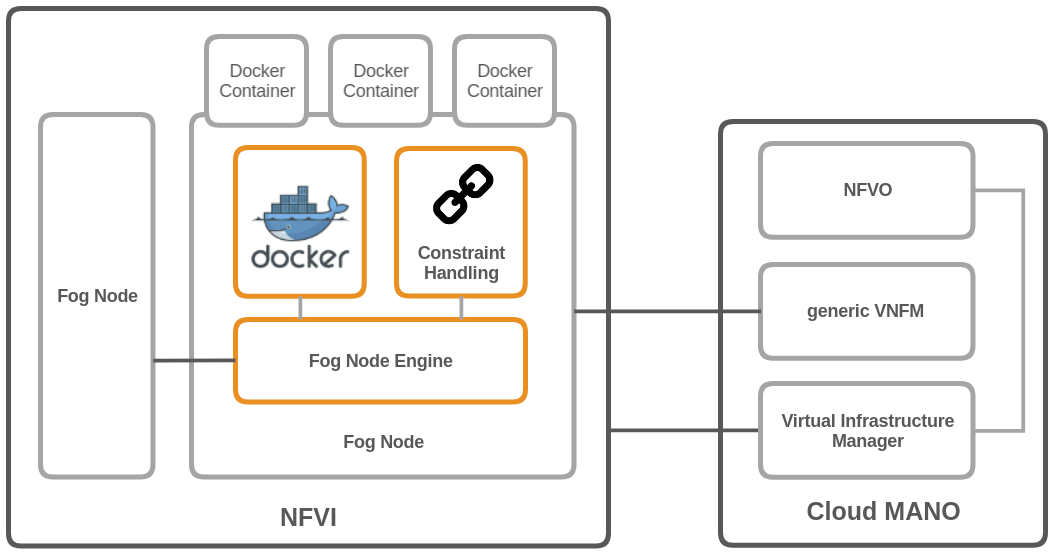
\includegraphics[width=0.85\textwidth]{resources/images/conceptual_architecture.png}
    \caption[Conceptual architecture based on a draft of the FOKUS]{Conceptual architecture based on a draft of the \ac{FOKUS}}
    \label{fig:conceptual_architecture}
\end{figure}

Figure \ref{fig:conceptual_architecture} shows a conceptual architecture design that is based on a draft of the \ac{FOKUS}.
On the right side is the abstract cloud infrastructure.
This could be for example Open Baton or any other \ac{MANO} compliant Framework.
The cloud infrastructure will be considered while developing the prototype, but the development or integration of such a component is out of scope for this thesis.
The \ac{NFVI} on the left side includes the Fog Node.
A single fog node should have the fog node engine, which is the prototype to be developed, as well as the Docker engine.
The constraint handling is part of the fog node engine and the concrete implementation has to be elaborated.
The fog node engine can orchestrate the local Docker containers, or if it necessary, it can move containers over to one or multiple other fog nodes.
This allows the system to be more flexible and it can achieve an autonomous orchestration level.
The autonomous orchestration of containers between fog nodes, without an existing connection to the cloud server, is desirable, but not part of this thesis.
Due to the fact that the prototype will be used in an \ac{IoT} context, the system will be tested on low power devices, for example on a Raspberry Pi\footnote{\url{https://www.raspberrypi.org}} cluster.
It is out of scope to create a system that guarantees to be executable on arbitrary devices, but theoretically this could be achieved by using a platform independent programming language and corresponding frameworks.


\section{Outline}
In chapter \ref{chapter:state-of-the-art} an introduction is given to relevant topics like the \ac{IoT} in the context of Industry 4.0, \acp{CPS} and Fog Computing as subtopics, virtualization, especially container virtualization and orchestration and \ac{NFV}.
Followed by a comparison of several established tools available on the market and some messaging concepts like \ac{MQTT} and ZeroMQ.
The section will be finalized by an overview of realted work.
The definition of the requirements as well as features and capabilities of the prototype will be shown in chapter \ref{chapter:requirements-analysis}.
Based on that, the architecture of the system is illustrated in chapter \ref{chapter:concept}.
The proof-of-concept implementation will be worked out in chapter \ref{chapter:implementation} and the functionality of the plugin will be demonstrated.
Chapter \ref{chapter:evaluation} summarizes the results of the work and evaluates the viability in terms of software quality, usability and feature-completeness.
Finally the gathered insights as well as an outlook for further improvements of the plugin will be argued in chapter \ref{chapter:conclusion}.
% TODO: can be more detailed

% The ’structure’ or ’outline’ section gives a brief introduction into the main chapters of
% your work. Write 2-5 lines about each chapter. Usually diploma thesis are separated
% into 6-8 main chapters.
% This example thesis is separated into 7 chapters.
% Chapter 2 is usually termed ’Related Work’, ’State of the Art’ or ’Fundamentals’.
% Here you will describe relevant technologies and standards related to your topic. What
% did other scientists propose regarding your topic? This chapter makes about 20-30 percent
% of the complete thesis.
% Chapter 3 analyzes the requirements for your component. This chapter will have
% 5-10 pages.
% Chapter 4 is usually termed ’Concept’, ’Design’ or ’Model’. Here you describe your
% approach, give a high-level description to the architectural structure and to the single
% components that your solution consists of. Use structured images and UML diagrams
% for explanation. This chapter will have a volume of 20-30 percent of your thesis.
% Chapter 5 describes the implementation part of your work. Don’t explain every code
% detail but emphasize important aspects of your implementation. This chapter will have
% a volume of 15-20 percent of your thesis.
% Chapter 6 is usually termed ’Evaluation’ or ’Validation’. How did you test it? In
% which environment? How does it scale? Measurements, tests, screenshots. This chapter
% will have a volume of 10-15 percent of your thesis.
% Chapter 7 summarizes the thesis, describes the problems that occurred and gives an
% outlook about future work. Should have about 4-6 pages.

% write about the research outline and Figure 1.6. Summarize Chapters 1 to 8

% Gute Quelle:
% http://winfwiki.wi-fom.de/index.php/Wertsch%C3%B6pfungsnetzwerke_und_Industrie_4.0

% Masterarbeit Alex
% https://www.yumpu.com/de/document/view/21142108/schriftliche-ausarbeitung-alexander-willner-masterarbeit/5

% https://de.slideshare.net/KarlIsenberg/container-orchestration-wars

\chapter{State of the art}\label{chapter:state-of-the-art}
This chapter will give an overview into the background and concepts of this thesis.
In the first section the \ac{IoT} an related subtopics like smart factories and Smart Cities are considered.
\acp{CPS}, which are important for the development of smart factories are also covered in this section.
Virtualization in general is the main topic of the second section.
First we dive into the area of \acp{VM}, followed by Container Virtualization.
Both are related to each other and sharing some basic ideas.
Container Orchestration as an own subsection show some possibilities of Container Virtualization.
The last subsection \ac{NFV} concludes with an introduction into the virtualization of network node functions to create communication services.
\todo{Rework that section}


\section{Internet of Things}
The \ac{IoT} has been a subject of great media- and economically growth in the recent years.
In the year 2008 the number of devices which are connected to the Internet was higher than the human population.\cite[cf.][p. 3]{Eva:2011}
Cisco Internet Business Solutions Group predicted that the number will grow up to 50 billion in 2020, this equates to around 6 devices per person.\cite[cf.][p. 4]{Eva:2011}
Most of today\'s interactions are \ac{H2H} or \ac{H2M} communication.
The \ac{IoT} on the other hand aim for the \ac{M2M} communication.
This allows every physical devices to be interconnected and to communicate with each other.
These devices are also called "Smart Devices".
Creating a network where all physical objects and people are connected via software is one primary goal of the \ac{IoT}.\cite[cf.][p.206]{Rui:2015}\cite[cf.][p.2]{Kra:2013}
When objects are able to capture and monitor their environment, a network can perceive external stimuli and respond to them.\cite[cf.][p. 40]{Itu11}
Therefore a new dimension of information and communication technology will be created, where users have access to everything at any time, everywhere.
In addition to smart devices, subcategories are also emerging from the \ac{IoT} which, in addition to the physical devices, also describe technologies such as protocols and infrastructures.
The "Smart Home" has been a prominent topic in media and business for many years.
Smart City or Industrie 4.0 are also becoming established and are increasingly popular.
But the Internet started with the appearance of bar codes and \ac{RFID} chips.\cite[cf.][p. 13]{Kra:2013}
The second step, which is more or less the current situation, sensors, physical devices, technical devices, data and software are connected to each other.\cite[cf.][p. 13]{Kra:2013}
This was achieved, in particular, by cloud computing, which provides the highly efficient memory and computing power that is indispensable for such networks.\cite[cf.][p. 206]{Rui:2015}
The next step could be a "Cognitive Internet of Things", which enables easier object and data reuse across application areas, for example through interoperable solutions, high-speed Internet connections and a semantic information distribution.\cite[cf.][p. V]{Kra:2013}
Just as the omnipresent information processing in everyday life, also known as "Ubiquitous Computing", which was first mentioned in the "The Computer for the 21st Century"\autocite{Wei:1991} by Marks Weiser, it will take some time until it is ubiquitous.


\subsection{Industry 4.0 and smart factories}
The industry as an changing environment is currently in the state of the so called "fourth industrial revolution".
The first industrial revolution was driven by steam powered machines.
Mass production and division of labor was the primary improvement of the second industrial revolution, whereas the third revolution was characterized by using electronics and the integration of \ac{IT} into manufacturing processes.\cite[cf.][p. 1]{Lom:2016}
In the recent years the size, cost and power consumption of chipsets are reduced which made it possible to embed sensors into devices and machines much easier and cheaper.\cite[cf.][p. 1]{Brito:2016}
The Industry 4.0 is the fourth step in this evolution and was first mentioned with the German term "Industrie 4.0" at the Hannover Fair in 2011.\cite[cf.][p. 1]{Lom:2016}
"Industrie 4.0 is a collective term for technologies and concepts of value chain organization."\cite[cf.][p. 11]{Her:2015}

Significantly higher productivity, efficiency, and self-managing production processes where everything from machines up to goods can communicate and cooperate with each other directly are the visions of the Industry 4.0.\cite[cf.]{Lyd:2016}
It also aims for an intelligent connection between different companies and units.
Autonomous production and logistics processes creating a real-time lean manufacturing ecosystem that is more efficient and flexible.\cite[cf.]{Lyd:2016}
"This will facilitate smart value-creation chains that include all of the life-cycle phases of the product from the initial product idea, development, production, use, and maintenance to recycling."\autocite{Lyd:2016}
At the end, the system can use customer wishes in every step in the process to be flexible and responsive.\cite[cf.]{Lyd:2016}

\taburulecolor{ob_dark_gray}
\begin{table}[htpb]
  \centering
    \begin{tabular}{| r | c c c c |}
      \rowcolor{ob_orange}
      \hline
                            & Cyber-Physical & Internet  & Internet    & Smart Factory \\
      \rowcolor{ob_orange}
                            & Systems        & of Things & of Services &  \\
      \hline
      Interoperability      & X        & X        & X          & X    \\
      Virtualization        & X        & -        & -          & X    \\
      Decentralization      & X        & -        & -          & X    \\
      Real-Time Capability  & -        & -        & -          & X    \\
      Service Orientation   & -        & -        & X          & -    \\
      Modularity            & -        & -        & X          & -    \\
      \hline
    \end{tabular}
  \caption[Design principles of each Industry 4.0 component]{Design principles of each Industry 4.0 component.\cite[cf.][p. 11]{Her:2015}}
  \label{tab:industryComponents}
\end{table}

Table \ref{tab:industryComponents} shows the six design principles which can be from the Industrie 4.0 components.
They can help companies to identify and implement Industry 4.0 scenarios.\cite[cf.][p. 11]{Her:2015}

\begin{enumerate}
  \item \textit{Interoperability} \ac{CPS} of various manufacturers are connected with each other. Standards will be the key success factor in this area.\cite[cf.][p. 11]{Her:2015}
  \item \textit{Virtualization} \ac{CPS} are able to monitor physical processes via sensors. The resulting data is linked to virtual plant and simulation models. These models are virtual copies of physical world entities.\cite[cf.][p. 11]{Her:2015}
  \item \textit{Decentralization} \ac{CPS} are able to make decisions on their own, for example when \ac{RFID} chips send the necessary working steps to the machine. Only in cases of failure the systems delegate task to a higher level.\cite[cf.][p. 11]{Her:2015}
  \item \textit{Real-Time Capability} Data has to be collected and analyzed in real time and the status of the plant is permanently tracked and analyzed. This enables the \ac{CPS} to react to a failure of a machine and can reroute the products to another machine.\cite[cf.][p. 11]{Her:2015}
  \item \textit{Service Orientation} \ac{CPS} are available over the \ac{IoS} and can be offered both internally and across company borders to different participants. The manufacturing process can be composed based on specific customer requirements.\cite[cf.][p. 11]{Her:2015}
  \item \textit{Modularity} The system is able to be adjusted in case of seasonal fluctuations or changed product characteristics, by replacing or expanding individual modules.\cite[cf.][p. 11]{Her:2015}
\end{enumerate}

Another important aspect of Industry 4.0 is the implementation of process automation with the focused on three distinct aspects.
Starting with the vertical integration, which contains the connection and communication of subsystems within the factory enables flexible and adaptable manufacturing systems.\cite[cf.][p. 7 ff.]{Vbw:2014}
The horizontal integration, as the second aspect, enables technical processes to be integrated in cross-company business processes and to be synchronized in real time through multiple participants to optimize value chain outputs.\cite[cf.][p. 7 ff.]{Vbw:2014}
Finally end-to-end engineering, planning, and process control for each step in the production process.\cite[cf.]{Lyd:2016}

\begin{figure}[H]
    \centering
    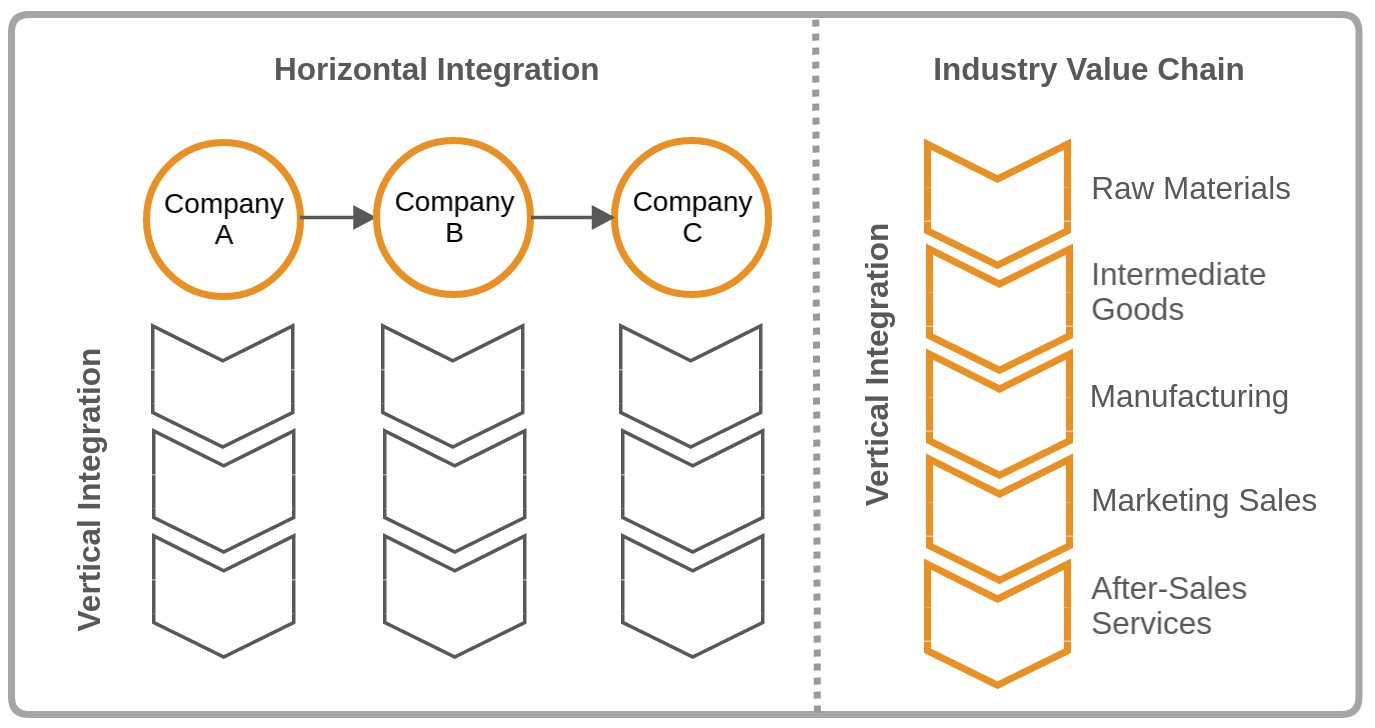
\includegraphics[width=\textwidth]{resources/images/vertical_horizontal_integration.png}
    \caption[Horizontal vs. Vertical Integration]{Horizontal vs. Vertical Integration. Adapted from: \autocite{Jur:2013}}
    \label{fig:vertical_horizontal_integration}
\end{figure}

Figure \ref{fig:vertical_horizontal_integration} illustrates this concept.
The left side shows the whole production process over company boundaries on the horizontal scale, as well as the industry value chain on the vertical scale which is specific for each company.
On the right side there is an exemplary industry value chain which starts with the raw materials and ends with the sale of the product to illustrates an more specific example of the vertical integration.
From a technical site this means each machine in a factory has exactly to know what they have to do.
The underlying system has to be modular and move away from a monolithic centralized system, to a decentralized system which is located locally near the machines himself.
The communication path between them have to grow shorter.
The machines have to be self organized and should communicate between each other even if the core system is not reachable because of lossy signals or other connection issues.
If this can be achieved there will be an highly flexible, individualized and resource friendly mass production, which can be cheaper, faster and can have a much higher fault tolerance.


\subsection{Cyber Physical Systems}
As we already now, in smart factories every physical device is connected to each other.
Everything can be captured and monitored in each step of a production process.
With \acp{CPS} every physical entity has a digital representation in the virtual system.\cite[cf.][p. 1363]{Poovendran:2010}
Before a \ac{CS} was passive, which means there was no communication between the physical and the virtual world.\cite[cf.][p. 1364]{Poovendran:2010}
While new technologies in the physical world, like new materials, hardware and energy, are developed, the technologies in the virtual worlds are also being improved, for example through the use of new protocols, networking, storage and computing technologies.\cite[cf.][p. 1364]{Poovendran:2010}
This adds more intelligence in such systems, as well as a much more flexible and modular structure.
A \ac{CPS} can organize production automatically and autonomously, which eliminate the need of having a central process control.\cite[cf.]{Lom:2016}
Thereby the system can handle lossy signals and short range radio technologies, which are widely used in such a context.\cite[cf.]{Yannuzzi:2014}
In summary \acp{CPS} can help to enable the vision of smart factories in both the horizontal as well as the vertical integration.


\subsection{Fog Computing}
In the beginning of Cloud Computing most of the systems based on a monolithic architecture.
Over time the system was broken down to a more distributes multicloud architecture, similar to microservices.
With the appearance of Fog Computing the Cloud also moves from centralized data centers to the edge of the underlying network.
Main goal is to improve the efficiency, reduce the traffic and the amount of data which is transferred to the cloud and also process, analyze and store data locally, as well as keeping sensitive data inside the network for security reasons.\cite[cf.][p. 236]{Brito:2016}\cite[cf.][p. 325]{Yannuzzi:2014}\cite[cf.][p. 4]{Lom:2016}
In contrast to the goals the definition and understanding of Fog Computing differs.
One perspective is to that the processing of the data take place on smart devices, e.g. sensors, embedded systems, etc., at the end of the network or in smart router or other gateway devices.\cite[cf.][p. 4]{Lom:2016}
Another interpretation is that fog computing appears as an intermediate layer between smart devices and the cloud.\cite[cf.][p. 236]{Brito:2016}
Processing the data near devices enables lower latency and real-time applications can take decisions based on analytics running there.
That is important because a continuous connection to the cloud can not always be ensured.
However fog computing should not be seen as a competitor of cloud computing, it is a perfect ally for use cases where cloud computing alone is not feasible.\cite[cf.][p. 325]{Yannuzzi:2014}


\section{Virtualization}
According to the \ac{NIST} the definition of virtualization is: "Virtualization is the simulation of the software and/or hardware upon which other software runs. This simulated environment is called a virtual machine (VM)."\cite[p. ES-1]{Sca:2011}.
This means a \ac{VM}, also referred as guest system, can be executed in a real system, which is referred as host system.
A \ac{VM} has its own \ac{OS} which is completely isolated from the other \acp{VM} and the host system.\cite[cf.][p. 2]{Celesti:2016}
Basically there are two types of virtualization: Process virtualization where the virtualizing software also known as \ac{VMM} is executed by the host \ac{OS} and only an application will be executed inside the guest \ac{OS} and on the other side there is the the system virtualization where the whole \ac{OS} as well as the application are running inside the virtualizing software.
Figure \ref{fig:vms_vs_docker} illustrate both concepts.
Examples for process virtualization could be the \ac{JVM}\footnote{\url{https://www.java.com}}, the .Net framework\footnote{\url{https://www.microsoft.com/net}} or Docker\footnote{\url{https://www.docker.com}}, where VMWare\footnote{\url{http://www.vmware.com}}, Oracle Virtual Box\footnote{\url{https://www.virtualbox.org}}, XEN\footnote{\url{https://www.xenproject.org}} or Microsoft Hyper-V\footnote{\url{https://www.microsoft.com/de-de/cloud-platform/server-virtualization}} are only some examples for system virtualization.
The benefits of all virtualization techniques are the rapid provisioning of resources which could be \ac{RAM}, disk storage, computation power or network bandwidth.
Beside that, no human interaction is necessary during the provisioning process.
Elasticity which scales a system in a cost-efficient manner in both directions, up and down.
Customer as well as the provider profit from such a system.
Security based on the isolation of the \acp{VM} is another huge benefit.
Different processes can not interfere with each other and the data of a single user can not be accessed by other users of the same hardware.
A challenge despite all the mentioned benefits is the performance.
Running \acp{VM} increases the overhead and reduces the overall performance of a system.
Therefore the specific use case have to consider these behavior.

\begin{figure}[H]
    \centering
    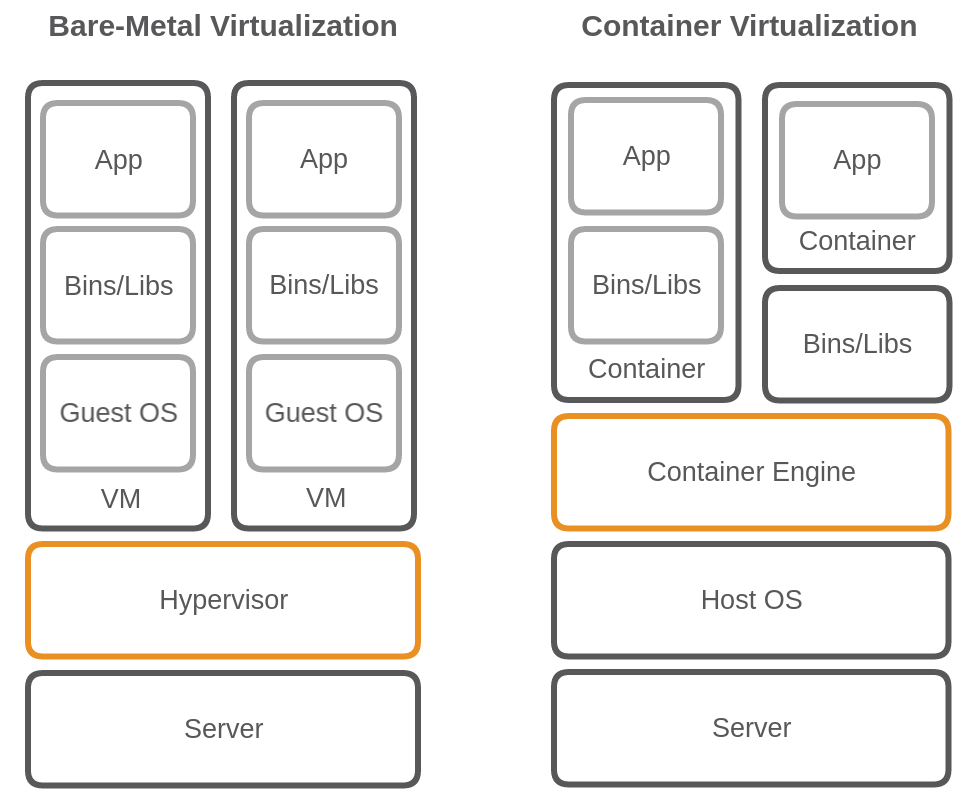
\includegraphics[width=0.6\textwidth]{resources/images/vm_vs_container.png}
    \caption[Structure bare-metal virtualization vs. container virtualization]{Structure bare-metal virtualization vs. container virtualization. Adapted from: \cite[p. 2]{Gallagher:2015}}
    \label{fig:vms_vs_docker}
\end{figure}


\subsection{Virtual Machines}
\acp{VM} are the core virtualization mechanism in cloud computing.
There are also two different designs for hardware virtualization.
The first and more popular type for cloud computing is the \textit{bare-metal virtualization}.
It needs only a basic OS to schedule \acp{VM}.
The hypervisor runs directly on the hardware of the machine without any host \ac{OS} in between.
This is more efficient, but requires special device drivers to be executed.
The other type is the \textit{hosted virtualization}.
Unlike the first type the \ac{VMM} run as a host \ac{OS} process and the \acp{VM} as a process supported by the \ac{VMM}.
No special drivers are needed for these type of virtualization, but by comparison the overhead is much bigger.
For both types, the performance limitation remains.
Each \ac{VM} need a full guest \ac{OS} image in addition to binaries and libraries which are necessary for the application to be executed.\cite[cf.][p. 381]{Pahl:2015}
If only a single application, which only needs a few binaries and libraries, is needed to be virtualized, \acp{VM} are too bloated.


\subsection{Container Virtualization}
Container virtualization which is also known as Operating System-level virtualization, is the second virtualization mechanism.
It based on fast and lightweight process virtualization to encapsulate an entire application with its dependencies into a ready-to-deploy virtual container.\cite[cf.][p. 72]{Tosatto:2015}
Such a container can be executed on the host \ac{OS} which allows an application to run as a sand-boxed user-space instance.\cite[cf.][p. 1]{Anderson:2016}
All containers share a single \ac{OS} kernel, so the isolation supposed to be weaker compared to hypervisor based virtualization.\cite[cf.][p. 2]{Celesti:2016}
Compared to \acp{VM}, the number of containers on the same physical host can be much higher, because the overhead of a full \ac{OS} virtualization is eliminated.\cite[cf.][p. 2]{Celesti:2016}


\subsection{Container Orchestration}
Containers by itself helps to develop and deploy applications, but containers release their full potential only when they are used together with an orchestration engine.
Before orchestration engines, the deployment of an application or service was realized via \ac{CI} and deployment tools like Vagrant or Ansible.
Deployment scripts or plans was created and be executed every time an application changed or should be scaled up on a new machine.
This was less flexible and error-prone.
Orchestration engines cover these needs by automatically choosing new machines, deploying containers, handle the lifecycle of them and monitor the system.
These flexibility enables a new level of abstraction and automatization of deployment.
There are a bunch of orchestration engines out there.
For Docker, Kubernetes and Docker Swarm are the most popular at the moment.


\subsection{Network Function Virtualization}
\ac{NFV} is an architectural framework to provide a methodology for the design, implementation, and deployment of \acp{NF} through software virtualization.\cite[cf.][p. 8]{ETSI:NFV:2013}\cite[cf.]{Rivenes:2014}
"These \acp{NF} are referred as \acp{VNF}."\cite[p. 8]{ETSI:NFV:2013}
It takes into consideration \ac{SDN} and preparing for the use of non-proprietary software to hardware integration instead of multiple vendor specific devices for each function, e.g. routers, firewalls, storages, switches, etc.\cite[cf.]{Rivenes:2014}
Now high-performance firewalls and load balancing software for example can run on commodity PC hardware and traffic can be off-loaded onto inexpensive programmable switches.\cite[cf.]{Noble:2015}

\begin{figure}[H]
    \centering
    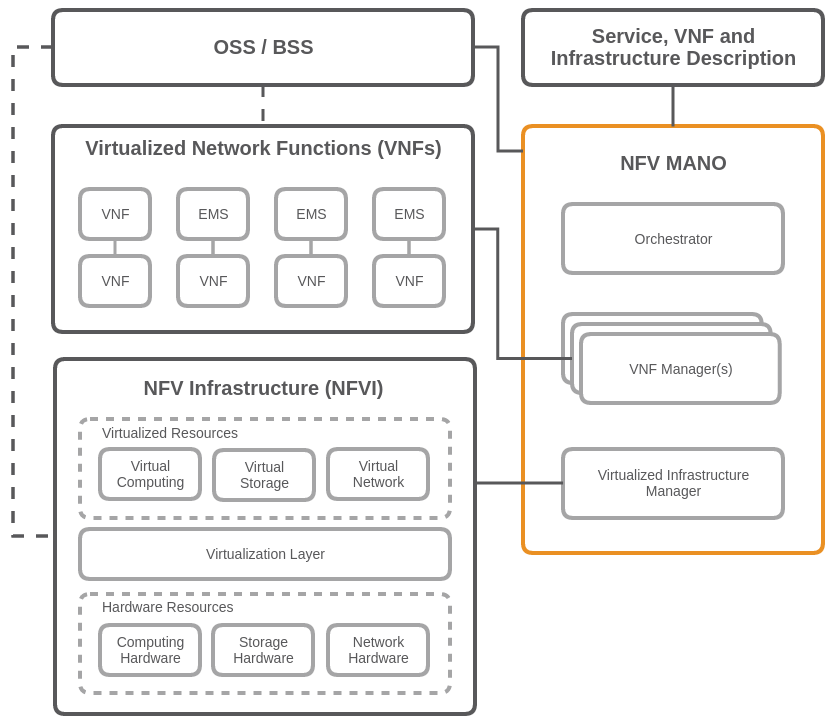
\includegraphics[width=0.75\textwidth]{resources/images/nfv_architecture.png}
    \caption[NFV architecture]{NFV architecture. Adapted from: \autocite{NFV:Architecture}}
    \label{fig:nfv_architecture}
\end{figure}

Some benefits are speed, agility and cost reduction in deployment as well as execution manner.\cite[cf.]{Noble:2015}
Using homogeneous hardware simplifies the process of planning and reduces power, cooling and space needs.\cite[cf.]{Noble:2015}
Through virtualization providers can utilize resources more effectively, by allocating only the necessary resources for a specific functionality.\cite[cf.]{Noble:2015}
Overall \ac{NFV} can reduce \ac{OpEx} as well as \ac{CapEx} and can decreasing the time necessary to deploy new services to the network.\cite[cf.]{Noble:2015}
To achieve \ac{NFV} the \ac{ETSI} has defined a framework the \ac{NFV-MANO}\footnote{\url{http://www.etsi.org/deliver/etsi_gs/NFV-MAN/001_099/001/01.01.01_60/gs_NFV-MAN001v010101p.pdf}} and the \ac{OASIS} created \ac{TOSCA} a \ac{NFV} specific data model and templates to coordinate and orchestrate the \ac{NF} into the cloud.

\paragraph{\acs{OSS} /\ \acs{BSS}} refers to the \ac{OSS} and the \ac{BSS} of a telecommunication operator.\cite[cf.]{Kahn:2015}
The \ac{OSS} is responsible for the underlaying soft- and hardware system, for example for network and fault management.
The \ac{BSS} on the other hand is responsible for the business handling, for example customer and product management.
Both can be integrated with the \ac{NFV-MANO}.\cite[cf.]{Kahn:2015}

\paragraph{\acp{VNF}} are the virtualized network elements, for example a virtualized router or virtualized firewall.
Even if only a sub-functions or a sub-components of a hardware element is virtualized, it is called \ac{VNF}.\cite[cf.]{Kahn:2015}
Multiple sub-functions can act together as one \ac{VNF}.

\paragraph{\ac{EMS}} is responsible for the functional management of a single or multiple \acp{VNF}.\cite[cf.]{Kahn:2015}
This includes fault, configuration, accounting, perfomance and security management.\cite[cf.]{Kahn:2015}
Furthermore the \ac{EMS} itself can be a \ac{VNF} or it can handle a \ac{VNF} through proprietary interfaces.\cite[cf.]{Kahn:2015}

\paragraph{\ac{NFVI}} is the environment where \acp{VNF} are executed.
This includes physical resources as well as virtual resources and the virtualization layer.
The physical resources could be a commodity switch, a server or a storage device.
These physical resources can be abstracted into virtual resources through the virtualization layer which is normally a hypervisor.
If the virtualization part is missing, the software runs natively on the hardware and the entity is no longer a \ac{VNF} it is then a \ac{PNF}.\cite[cf.]{Kahn:2015}

\paragraph{\ac{NFV-MANO}} consists of three main parts.
The \ac{VIM} is "responsible for controlling and managing the NFVI compute, network and storage resources within one operator’s infrastructure domain"\autocite{Kahn:2015}.
The \ac{VNFM} manages one or multiple \acp{VNF}.
This includes the life cycle management of the \ac{VNF} instances, such as instantiate, edit or shut down an \ac{VNF} instance.\cite[cf.]{Tosca:NFV}
In contrast to the \ac{EMS}, the \ac{VNFM} handles the virtual part of the \ac{VNF}, for example instantiate an instance, while the \ac{EMS} handles the functional part of an \ac{VNF}, such as issue handling for a \ac{VNF}.
The orchestrator as the third component in the \ac{NFV-MANO} block manage network services of \acp{VNF}.
It is responsible for the global resources management, such as computing and networking resources among multiple \acp{VIM}.\cite[cf.]{Kahn:2015}
The orchestrator interacts with the \ac{VNFM} to perform actions, but not with the \acp{VNF} directly.\cite[cf.]{Kahn:2015}
\ac{TOSCA} is often used with \ac{NFV-MANO} frameworks like Cloudify\footnote{\url{http://getcloudify.org}} or Open Baton.\cite[cf.]{Tosca:NFV}

\paragraph{\ac{TOSCA}} is developed by the \ac{OASIS} to deliver a declarative description of a \ac{NFV} application topology for network or cloud environments.\cite[cf.]{Tosca:NFV}
In figure \ref{fig:nfv_architecture} it is represented by the \textit{Service, VNF and Infrastructure Description} block.
Beside that, it can also be used to define workflows which should be automated in a virtualized environment.\cite[cf.]{Tosca:NFV}
The \ac{TOSCA} modeling language can specify ndoes, whereby a node can be a network, a subnet or only a server software component, and it also handles relationships between the nodes and also services.\cite[cf.]{Tosca:NFV}
To define schemas, relationships and the configuration of such an infrastructure, it uses \ac{YAML} files for ease the usage.\cite[cf.]{Tosca:NFV}
\ac{TOSCA} works pretty well with \ac{NFV-MANO} components to automate the deployment and management of \acp{NF} and services.


\section{Existing tools}

There are several advantages of using frameworks and sophisticated tools, for example they reduces the time and energy in developing any software, they are more secure, well tested and they provides a standardized system through which users can develop applications.
They also allow to create a prototype of an application in a short amount of time.
To achieve the benefits the user has to spend some time to learn the concepts, functions and how to use a framework.

\subsection{Linux Containers}
When we talk about container virtualization nowadays, Docker have to become one of the most famous tools out there.
It based on \ac{LXC}\footnote{\url{https://linuxcontainers.org/}} a technology which uses kernel mechanisms like \textit{namespaces} or \textit{cgroups} to isolate processes on a shared \ac{OS}.\cite[cf.][p. 381]{Pahl:2015}
Namespaces for example are used to isolate groups of processes whereas cgroups are used to manage and limit resources access just like restricting the memory, disc space or \ac{CPU} usage.\cite[cf.][p. 381]{Pahl:2015}
"The goal of \ac{LXC} is to create an environment as close as possible to a standard Linux installation but without the need for a separate kernel."\cite[p. 72]{Tosatto:2015}
There are several other container virtualization tools out there like OpenVZ\footnote{\url{https://openvz.org/Main_Page}} or Linux-VServer\footnote{\url{http://www.linux-vserver.org}}.
In contrast to them, an advantage of \ac{LXC} is that it runs on an unmodified Linux kernel.
This means that \ac{LXC} can be executed in most of the popular Linux distributions these days.

\subsection{Docker}
As mentioned before, Docker based on \ac{LXC}.
This allows the Docker Engine to build, deploy and run containers in an easy and customizable way.
Similar to \acp{VM}, containers are executed from images.
A mayor benefit of Docker is the fact, that Docker images can be combined like build blocks.
Each image can build on top of another.
Figure \ref{fig:docker_container_structure} illustrates the concept for the image of the pretty famous Django\footnote{\url{https://www.djangoproject.com/}} web framework.
In that case, the Django image, which is the resulting image, based on the Python 3.4 image which again based on the Debian Jessy image.
All of them are read-only, but Docker adds a writable layer, also known as \textit{container layer}, on top of the images as soon as the container will be created.
File system operations such as creating new files, modifying or deleting existing files are written directly to these layer.\cite[cf.]{dockerImages}
The other images don\'t get involved.
These chaining mechanism of images allows Docker to ease the use of dependencies and administrative overhead.

Beside that, Docker is split up in several components, such as the Docker Engine, the Docker Registries and Docker Compose to mention only a few.
The Docker Engine is a client-server application which can be distinguished by the Docker client, a \ac{REST} \ac{API} and the Docker server.
Latter is a daemon process which "creates and manages Docker objects, such as images, containers, networks, and data volumes"\autocite{dockerEngine}.
The client is a \ac{CLI}, which interact via a \ac{REST} \ac{API} with the daemon.\cite[cf.]{dockerEngine}

% Docker Registries
Another component, the Docker Registry, is basically a library of Docker images.
They can be public or private available, as well as on the same machine like the Docker daemon or an external server.\cite[cf.]{dockerEngine}
The most popular one it the official Docker Hub\footnote{\url{https://hub.docker.com}}.
There is also an Docker Store\footnote{\url{https://store.docker.com}}, where customers can buy and sell trusted and enterprise ready containers and plugins.
With the Docker client it is pretty easy to \textit{search} for new containers and to \textit{pull} containers from or \textit{push} containers to a specific repository.

\begin{figure}[H]
    \centering
    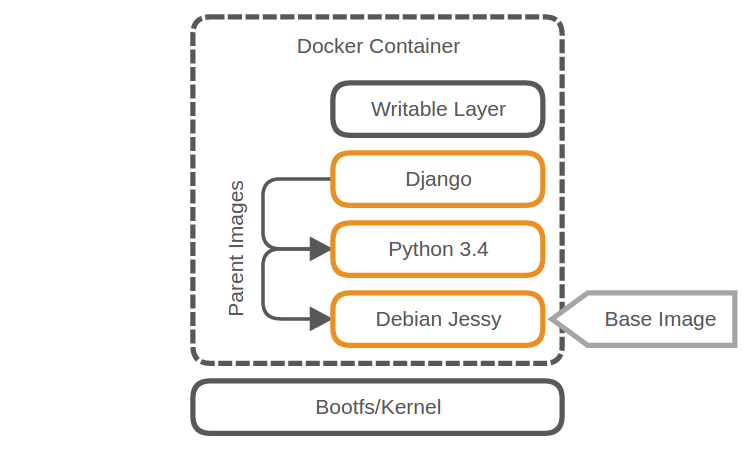
\includegraphics[width=0.75\textwidth]{resources/images/docker_container_structure.png}
    \caption[Docker container structure]{Docker container structure.}
    \label{fig:docker_container_structure}
\end{figure}

% Docker Compose
With Docker Compose multiple Docker Containers can be executed as a single application.
Therefore YAML compose file will be used to configure and combine the services.
For example the already mentioned Django image can be executed and linked together with a MongoDB\footnote{\url{https://www.mongodb.com}} images.
The main benefit is the ease of configure dependencies between several containers and configuration steps.
These concept is similar to deployment tools like Vagrant\footnote{\url{https://www.vagrantup.com}}, Ansible\footnote{\url{https://www.ansible.com}} or Puppet\footnote{\url{https://puppet.com}}.

% Benefits
A major benefit of Docker is that the execution environment of an application is completely the same on a local machine as on the production environment.\cite[cf.][p. 2]{Gallagher:2015}
There is no need to do things differently when switching from a development environment like a local machine, to a production environment like a server.\cite[cf.][p. 2]{Gallagher:2015}

\subsection{Kubernetes}
\label{subsection:state-of-the-art:kubernetes}
Kubernetes is an open source container cluster manager which was released 2014 by Google.
It is "a platform for automating deployment, scaling, and operations"\cite[p. 1]{Grant:2015} of containers.
Therefore a cluster of containers can be created and managed.
The system can for example schedule on which node a container should be executed, handle node failures, can scale the cluster by adding or removing nodes or enable rolling updates.\cite[p. 5 f.]{Grant:2015}

Figure \ref{fig:kubernetes_architecture} illustrates the basic architecture of Kubernetes.
The user can interact with the Kubernetes system via a \ac{CLI}, an \ac{UI} or a third party application, over a \ac{REST} \ac{API} to the Kubernetes Master or more specifically the \ac{API} Server in the master.
The master himself controls the one or multiple nodes, monitor the system, schedule resources or pull new images from the repository, to name only a few tasks.

\begin{figure}[H]
    \centering
    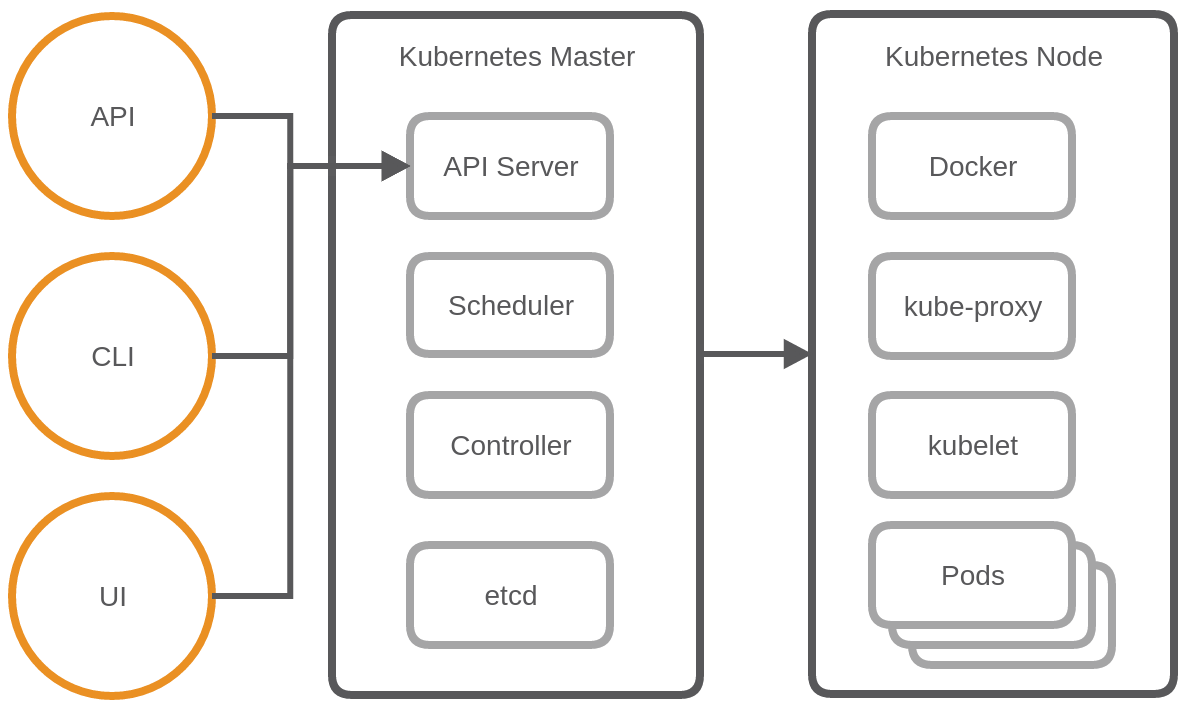
\includegraphics[width=0.75\textwidth]{resources/images/kubernetes_architecture.png}
    \caption[Kubernetes architecture]{Kubernetes architecture. Adapted from: \cite[p. 4]{MSV:2016}}
    \label{fig:kubernetes_architecture}
\end{figure}

Each node has a two way communication with the master via a kubelet.
In addition each node has the services necessary to run container applications like Docker.
Furthermore Kubernetes can combine one or multiple containers into one so called Pod.\cite[cf.][p. 7]{Mulyana:2016}
"Pods are always co-located and co-scheduled, and run in a shared context."\autocite{Kubernetes:pods:2016}
One node again can execute multiple Pods.
Pods are only temporary grouped containers with a non-stable \ac{IP} address.
After a Pod is destroyed it can never be resurrected.
Pods can also share functionality to other Pods inside a Kubernetes cluster.
A logical set of Pods and the access policy of them is called a Kubernetes service.
Such a service can abstract multiple Pod replicas and manage them.
A frontend which have access to the service do not care about changes in the service.
Any change, be it a down scale or an up scale of the system, remains unseen for the frontend.
They are exposed through internal or external endpoints to the users or the cluster.\cite[cf.][p. 11]{MSV:2016}
Labels can be used to organize and to select subsets of Kubernetes Objects, such as Pods or Services.\cite[cf.]{Kubernetes:labels:2016}
They are simply key-value pairs which and should be meaningful and relevant to users, but do not imply semantics to the core system.\cite[cf.]{Kubernetes:labels:2016}

The kube-proxy is a network proxy and load balancer which is accessible from the outside of the system via a Kubernetes service.\cite[cf.][p. 7]{Mulyana:2016}
"Each node and can do simple TCP,UDP stream forwarding or round robin TCP,UDP forwarding across a set of backends."\autocite{Kubernetes:kube-proxy:2016}
The Replication Controller is one of the mayor controllers in a Kubernetes System.
It ensures that a specified number of pod replicas are running and available at any time.\cite[cf.]{Kubernetes:replication-controller:2016}
If for example one node disappear because of connection issues, the Replication Controller will start a new one.
If the disappeared node is available back again it will kill a node.
These functionality increases the stability, the availability and the scalability of the system in an autonomous manner.
The last important component in Kubernetes are rolling updates.
With rolling updates the system can update one pod at a time, rather than taking down the entire service and update the whole system.\cite[cf.]{Kubernetes:rolling-updates:2016}
This also increases the stability and availability of the system and eases the managing of container clusters.

\subsection{Docker Swarm}
The basic functionality of Docker Swarm is pretty similar to Kubernetes: It is possible to create, manage and monitor a cluster of multiple machines running Docker on it.
Before Docker version 1.12.0, Docker Swarm was an independent tool, which is now integrated in the Docker Engine.\cite[cf.]{dockerSwarm}
No additional software is necessary to have a bunch of machines work together as a so called swarm.
Similar to Kubernetes, Docker Swarm needs a master node called manager and several worker nodes.
The manager for example keep track of the nodes and their lifecycle and it can start new instances of an image if one or multiple nodes disappear.
Furthermore Docker Swarm has a build in proxy and load balancer, which can redirect requests to the node with the necessary container running on it or redirect requests based on the workload of the machines.
Compared to Kubernetes, Docker Swarm is more lightweight, but misses some features like the label functionality or the schema definition of a pod.
But as mentioned before, both tools are pretty similar and aim for the same goal.


% \subsection{OpenStack}
% \doit
% "OpenStack is a cloud operating system that controls large pools of compute, storage, and networking resources throughout a datacenter"\autocite{OpenStackDoc}


% \subsection{Cloudify}
% Cloudify\footnote{\url{http://getcloudify.org}} is another open source orchestration tools created an israeli software company called GigaSpaces\footnote{\url{https://www.gigaspaces.com}} and was made primarily for the cloud.
% With Cloudify the creation of cloud services can be automated, starting by the deployment on pulic clouds like Amazon AWS or Microsoft Azure, over monitoring, failure detection and handling and ends in maintance of such a services.\cite[cf.]{Cloudify:Documentation}
% It also have a plugin mechanism which for example allows to use OpenStack, Puppet or Docker for the orchestration out of the box.
% Furthermore custom plugins can be created and integrated into the system.
% Cloudify can be completely controlled via a command line client or a webfronted.
% The latter provides a drag and drop \ac{GUI} to design and model application blueprint and is called Cloudify Composer.
% A blueprint describes an application in Cloudfiy, it is based on the \ac{TOSCA} standard and is written in \ac{YAML}.\cite[cf.]{Cloudify:Documentation}
% Basically a blueprint describes the single components like a webserver and a database of a system, how they relate to each other, how they should be installed and configured and finally how they should be monitored and maintained.\cite[cf.]{Cloudify:Documentation}
% Such a blueprint can be executed after they is created and will start the underlaying orchestration engine.
% Previously mentioned functionalities like auto-scaling, fault management and deployment over a huge cluster of nodes is also implemented.
% Since version 3.0 of Cloudify it also supports \ac{NFV} and delivers a couple of predefined blueprints\footnote{\url{http://getcloudify.org/examples/home.html}} for a seamless integration.
% Beyond that it is also used to deploy \ac{IoT} functions for example for an \ac{IIoT} environment\footnote{\url{http://www.livedatautilities.com/cloud-iiot-for-legacy-grids}}.
% Finally a couple of well known organizations are using Cloudify or Aria\footnote{\url{http://ariatosca.org}}, an open source fork of Cloudify for network providers that wants to build their own \ac{VNFM} and \ac{NFVO} tools, for example AT\&T, VMware or Deutsche Telekom.\cite[vgl.]{Hardesty:2016}


\subsection{Open Baton}
Open Baton\footnote{\url{https://openbaton.github.io}} is an open source \ac{ETSI} \ac{NFV} compliant \ac{MANO} Framework\cite[cf.]{openBatonDoc}.
"It enables virtual Network Services deployments on top of heterogeneous \ac{NFV} Infrastructures."\autocite{openBatonDoc}
It works together with OpenStack and provides a plugin mechanism which allows to add additional \acp{VIM}.\cite[cf.]{openBatonDoc}
In Open Baton it is implemented as the \ac{VIM} as first \ac{PoP} and uses the OpenStack \acp{API}.\autocite{openBatonDoc}
All the resources in the \ac{NFVI} are controlled by the \ac{VIM}, in this case OpenStack.

\begin{figure}[H]
    \centering
    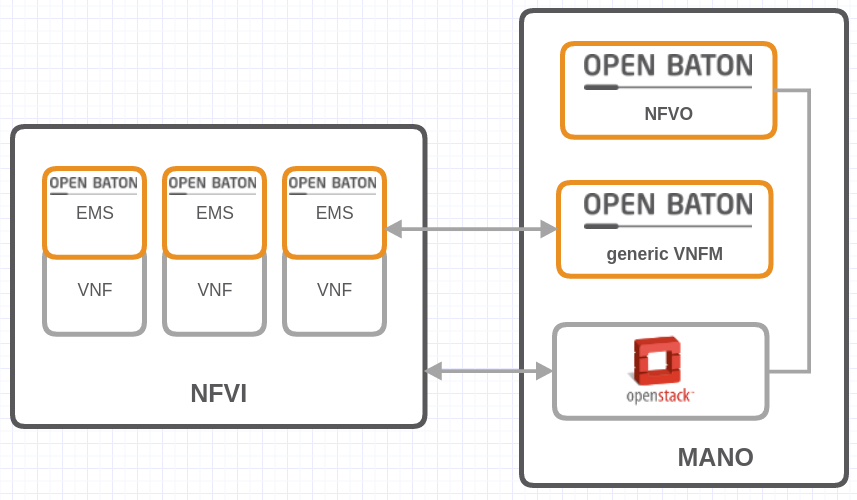
\includegraphics[width=0.75\textwidth]{resources/images/open_baton_simple_architecture.png}
    \caption[Open Baton abstract architecture]{Open Baton abstract architecture. Adapted from: \autocite{openBatonDoc}}
    \label{fig:open_baton_abstract_architecture}
\end{figure}

In the basic configuration Open Baton provides a generic \ac{VNFM} with generic \ac{EMS} related to the \acp{VNF}, but it can also be replaced with custom components.
The \ac{VNFM} can use a \ac{REST} \ac{API} or an \ac{AMQP} message queue to communicate with the system.
Figure \ref{fig:open_baton_abstract_architecture} illustrates the abstract architecture of Open Baton together with OpenStack and a generic \ac{VNFM}.
The \ac{NFVO} is completely designed and implemented as described in the \ac{ETSI} \ac{MANO} standard.\autocite{openBatonDoc}
It communicates with the \ac{VIM} to orchestrate resources and services and it is implemented as a separate module, so it can be replaced with a custom one if necessary.

A more detailed view of the Open Baton architecture is shown in figure \ref{fig:open_baton_detailed_architecture}.
As mentioned before each component communicate over the message queue and can be extended or replaced if necessary.
Additional components, such as the \ac{AE} or the \ac{FM} system, are provided to manage a network service at runtime.\autocite{openBatonDoc}
The necessary informations are delivered from the monitoring system available at the \ac{NFVI} level, which can also be extended or replaced with any monitoring system by implementing a custom monitoring driver.\autocite{openBatonDoc}
The \ac{VIM} Driver mechanism allows to replace OpenStack with external heterogeneous \acp{PoP}, but without the need of modifying the orchestration logic.\autocite{openBatonDoc}
Beside the generic \ac{VNFM}, also the Juju\footnote{\url{https://www.ubuntu.com/cloud/juju}} \ac{VNFM} can be used to deploy Juju Charms or Open Baton \ac{VNF} packages.
Open Baton also provides a marktplace\footnote{\url{http://marketplace.openbaton.org}} for free and open source \acp{VNF}, which can directly be loaded into the system.

Furthermore Open Baton comes with a modern and easy to use \ac{GUI} and user management.
The typical workflow of running a \ac{NFVI} is by starting them through the dashboard.
The user input, in this case deploying a \ac{VNF}, will be submitted as a request to the \ac{NFVO}.
There the orchestrator request the \ac{VIM}, for example OpenStack, to instantiate the network service.
The \ac{VIM} allocated the resources on the datacenter and starts the \acp{VM} based on the provided service description, for example through a \ac{TOSCA} description.
After the machines are finally booted, the \acp{EMS} will be installed to communicate with the \acp{VNFM}.
Open Baton now can send lifecycle events to all the \acp{VNFM} responsible for the \acp{VNF} which are part of the network service.
Finally the \acp{VNFM} processes the \acp{VNF} via the \ac{EMS} on to the given resources of the \ac{NFVI} on the datacenter.
The services are started and the system is up and running.

\begin{figure}[H]
    \centering
    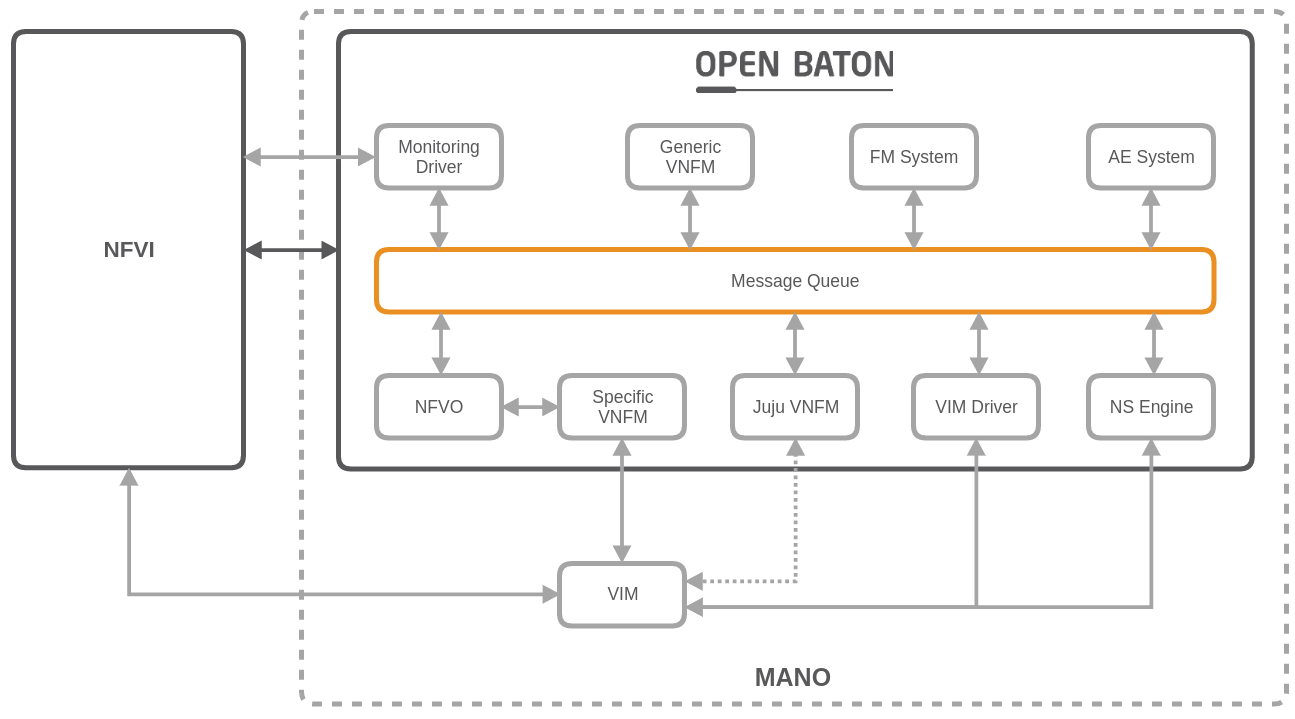
\includegraphics[width=\textwidth]{resources/images/open_baton_architecture.png}
    \caption[Open Baton detailed architecture]{Open Baton detailed architecture. Adapted from: \autocite{openBatonDoc}}
    \label{fig:open_baton_detailed_architecture}
\end{figure}

\section{Messaging}

\subsection{Message Queue Telemetry Transport}
\label{section:MQTT}
The \ac{MQTT} protocol formerly known as MQTT-S or MQTT-SN is a lightweight communication protocol developed by Andy Stanford-Clard and Arlen Nipper.\autocite[cf.]{MQTT:FAQ}
Meanwhile \ac{MQTT} is an \ac{OASIS} standard\footnote{\url{https://www.oasis-open.org/committees/tc_home.php?wg_abbrev=mqtt}}, which is often used in an \ac{IoT} and \ac{M2M} context.\autocite[cf.][p. 5]{lampkin:2012:mqtt}
It has a publish/subscribe architecture, which makes it easy to implement and allows thousands of remote clients to be connected to a single server at the same time.\autocite[cf.][p. 5]{lampkin:2012:mqtt}
The recipient of a message which is called consumer in the \ac{MQTT} context is completely decoupled from the sender, mostly called producer, via a broker.
In general the workflow is that a consumer subscribe to a specific topic at the broker and the producer can send messages with a specific topic to the broker.
The producer does not know if there is any consumer subscribed to the topic of a message.
The broker is resonsible for delivering messages to consumers, by receiving them from the producer and send out copies to the consumers.
Figure \ref{fig:mqtt_architecture} illustrates this concept.

In contrast to Client/Server protocols such as the \acs{HTTP}, \ac{MQTT} is eventoriented, which means that the client does not have to constantly ask the server if there is new data, the broker informs the consumer when there is new data on a topic.\autocite[cf.]{Bayer:MQTT}
In direct comparison, this concept decrease the traffic, the amount of connections at the server and the delay of the message to be send to the clients.

\begin{figure}[H]
    \centering
    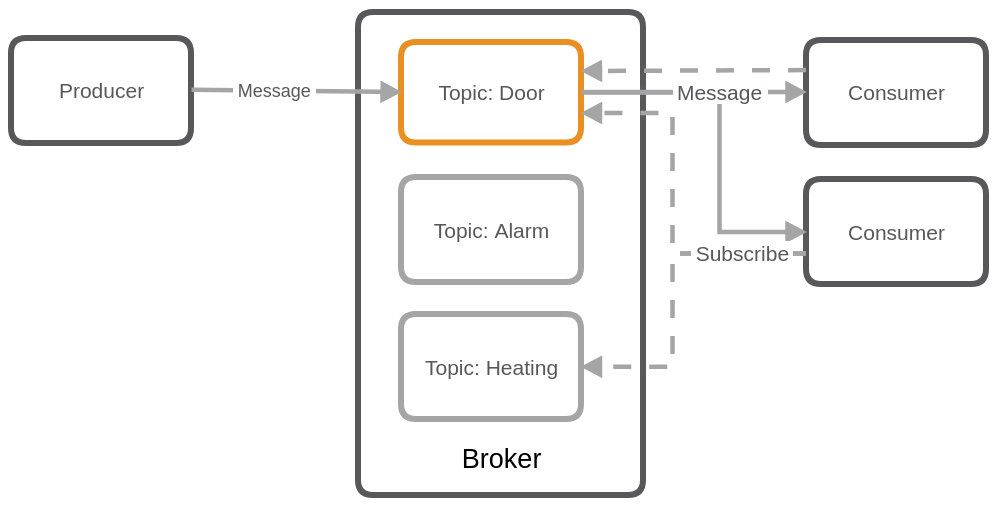
\includegraphics[width=0.75\textwidth]{resources/images/mqtt_architecture.png}
    \caption[MQTT publish/subscribe architecture]{MQTT publish/subscribe architecture. Adapted from: \autocite{Bayer:MQTT}}
    \label{fig:mqtt_architecture}
\end{figure}

Beside the publish/subscribe architecture and the lightweight protocol, \ac{MQTT} has only few but usful features.
\textbf{\ac{QoS}} define the level of reliability with which messages are delivered.\autocite[cf.]{Bayer:MQTT}
There are three different levels, where each level differs in reliability and resources usage.\autocite[cf.]{Bayer:MQTT}
In an \ac{IoT} context, for instance gathering temperature sensor data from a low power device, most of the time keeping the resources usage low is more important than the reliability of getting every single message.\newline
At \textit{\ac{QoS} level 0 - at most once}, it is garantied that a message can only arrieves once, but they can also be lost during transfer.
A single message will be send once and the publisher does not check the success of receiving them.
This pattern is also called \textit{Fire and Forget}, it is fast and resources friendly.\autocite[cf.]{Bayer:MQTT}\newline
At \textit{\ac{QoS} level 1 - at lest once}, it is grantied that a message will be received at the consumer.
After the publisher send the message with a specific packet identifier, the consumer will confirm the receipt of the message with a so called pubback packat.
The pubback packet also have the same packet identifier included, so that the publisher will know that the message was successfully delivered.
If a message get lost during transmission, they will be resend.
It is also possible, that the same message appears multiple times at the consumer, depending on the delay in the network.\newline
The most secure but also most resources consuming level is At \textit{\ac{QoS} level 2 - exactly once}.
At this level it is garantied, that a message is exactly received once.
It is not possible that a message appears multiple times or never.
This level has a two-level confirmation process, where at first the consumer confirms the receive of the message and afterwards the producers confirms the receive of the confirmation.
Therefor both sides can be sure to not send or receive duplicates and it is garantied that a message will be received.

Forthermore the broker has two features to handle connection loses: the \textit{last will testament} and the \textit{message persistence}.
The former feature will send a last message from the broker to a consumer if the connection to the publisher will get lost.
This could be for instances the information that the connection get lost or something similar.
The message persistance will be used if one consumer lose the connection to the broker.
In this case the message will be stored and delivered as soon as the consumer reconnects.
With the \textit{retrained messages} feature, a consumer which is connected for the first time to the broker will get the last message send for a specific topic. This can be useful if the temperature from a sensor should be displayed, but the value will only be fetched every 30 seconds. This would lead to the behaviour that the initial value on consumer side will in worst case be unknown for 30 seconds.
\textit{Persistent sessions} allows a connection be established even if the consumer disappers. In this case all the messages incurred will be stored and delivered if the consumer resume the session. The session can be identified with a unique client identifier.\autocite[cf.]{Bayer:MQTT}

Due to the fact that \ac{MQTT} is a simple protocol with a small footprint and the \ac{QoS} handshake enables the protocol to be independent from \acs{TCP} so that it can be used even on devices without a TCP/IP stack like embedded devices such as an Arduino.\autocite[cf.]{Bayer:MQTT}
There the protocol can be used via a bus or a serial port.\autocite[cf.]{Bayer:MQTT}
\ac{MQTT} himself support the protection of the messages via username nad password and the communication can be encrypted with \acs{SSL} or \acs{TLS} on the transport layer.\autocite[cf.]{Bayer:MQTT}
The broker can additionally use client certificates to authenticate them or restrict the access via access conrol lists such as \acs{IP} filtering.\autocite[cf.]{Bayer:MQTT}
\ac{MQTT} is available for most of the common programming languages and platforms.

% https://www.predic8.de/mqtt.htm
% https://blogs.vmware.com/vfabric/2013/02/choosing-your-messaging-protocol-amqp-mqtt-or-stomp.html

\subsection{ZeroMQ}
\label{section:ZeroMQ}
ZeroMQ is an messaging and communication framework to send atomic messages between applications and processec across various transports like \ac{TCP}, in-process, inter-process or multicast.\autocite[cf.]{ZeroMQ:Guide}
Every message will be send over sockets via several patterns like publish-subscribe, fan-out or a simple request-reply.\autocite[cf.]{ZeroMQ:Guide}
ZeroMQ has an asynchronous I/O model which allows to create high-performance and scalable multicore applications.\autocite[cf.]{ZeroMQ:Guide}
To distinguish it from messaging frameworks like \ac{AMQP}\footnote{\url{https://www.amqp.org}} ZeroMQ has no dedicated broker inbetween.
The benefit is that there is no single point of failure, not bottleneck and no need to maintain another component, but ZeroMQ still has the advantages of such a messaging system.

ZeroMQ supports five different transport types.\newline
\textbf{In-Process} is used for local (in-process or inter-thread) communication transport.
This transport passes the messages directly via memory between threads.\autocite[cf.]{ZeroMQ:inproc}
These transport type is optimal for creating multithreaded applications without providing access to the outside.
This is the fastes tranport type available in ZeroMQ.\newline
\textbf{\ac{IPC}} provides also a local communication transport, but passes messages via the \ac{OS} dependend \ac{IPC} machanism, for example UNIX domain sockets.
An application can provide a local \ac{API} for another local appliction via \ac{IPC}.
Also \ac{IPC} is much faster than the \ac{TCP} communication.\newline
\textbf{\ac{TCP}} is an ubiquitous, reliable, unicast transport to provide an \ac{API} over a network.\autocite[cf.]{ZeroMQ:tcp}\newline
\textbf{\ac{PGM}} is a multicast communication transport using the \ac{PGM} standard protocol\footnote{\url{https://tools.ietf.org/html/rfc3208}} and the datagrams are layered directly on top of IP datagrams.\autocite[cf.]{ZeroMQ:pgm}
It is helpful to send a squence of packets to multiple consumers at the same time.
Therefore \ac{PGM} and also \acs{EPGM} can only be used with the publish/subscribe pattern.\newline
\textbf{\ac{EPGM}} is similar to \ac{PGM} but with the difference that the PGM datagrams are encapsulated inside UDP datagrams.\autocite[cf.]{ZeroMQ:pgm}

ZeroMQ has serveral basic patterns and most of them are combinable.
To describe them all in detail would exceed the scope of this work, so only the most relevant ones are considered.\newline
\textbf{Request-Reply} is comparable with a \ac{HTTP} request-response.
The client send a message to the server, which does some work and send back a message afterwards.
It is represented by the REQ-REP socket pairs in ZeroMQ.
Figure \ref{fig:zeromq_req_rep} illustrates the pattern.\newline
\begin{figure}[H]
    \centering
    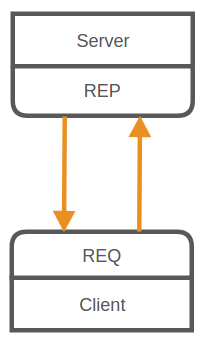
\includegraphics[width=0.25\textwidth]{resources/images/zeromq-req-rep.png}
    \caption[ZeroMQ Request-Reply architecture]{ZeroMQ Request-Reply architecture. Adapted from: \autocite{ZeroMQ:Guide}}
    \label{fig:zeromq_req_rep}
\end{figure}
The \textbf{Publish-Subscribe} pattern in ZeroMQ is basically comparable with the MQTT publish-susbcribe pattern, but without the broker inbetween.
This ends up in the fact that every consumer has to now the publisher and has to connect to them.
A direct connection between them will established.
Similar to MQTT, the publisher will send out the message to every subscribed consumer.
It is also possible to subscribe to more than one topic.
In ZeroMQ this pattern is represented by PUB-SUB socket pairs.
Figure \ref{fig:zeromq_pub_sub} shows this pattern.
\begin{figure}[H]
    \centering
    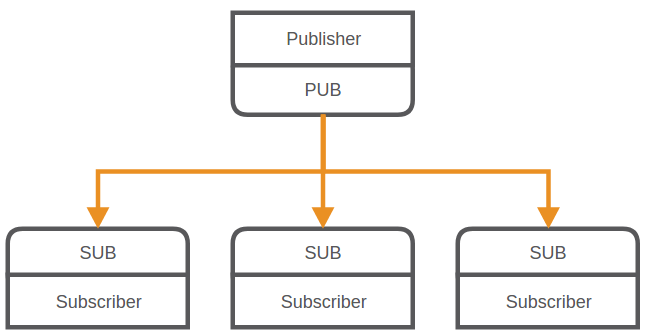
\includegraphics[width=0.6\textwidth]{resources/images/zeromq-pub-sub.png}
    \caption[ZeroMQ Publish-Subscribe architecture]{ZeroMQ Publish-Subscribe architecture. Adapted from: \autocite{ZeroMQ:Guide}}
    \label{fig:zeromq_pub_sub}
\end{figure}
The \textbf{Pipeline} pattern is also known as the \textit{Divide and Conquer} pattern.
There we have Ventilator which produces multiple tasks that can be done in parallel, a set of worker that can process these tasks and a sink that collects the results from the workers.\autocite{ZeroMQ:Guide}
Benefit of this pattern is, that the workers devide the tasks, this means it will increase the calculation time based on the connected workers.
FUrthermore the works can pull a new task if they are done.
This means a worker has a minimal idle time.
Queuing is provided by ZeroMQ.
It is also possible to add and remove workers dynamically.
This makes an application much more scalable.
Finally the sink pull the data from the worker in a so called \textit{fair-queuing}.
This means the sink will pull one package from each worker one after another, then he starts from the beginning and will pull again only one package, even if one or multiple worker should have multiple packages retrievable.
The whole pattern is shown in figure \ref{fig:zeromq_pipeline}\newline
\begin{figure}[H]
    \centering
    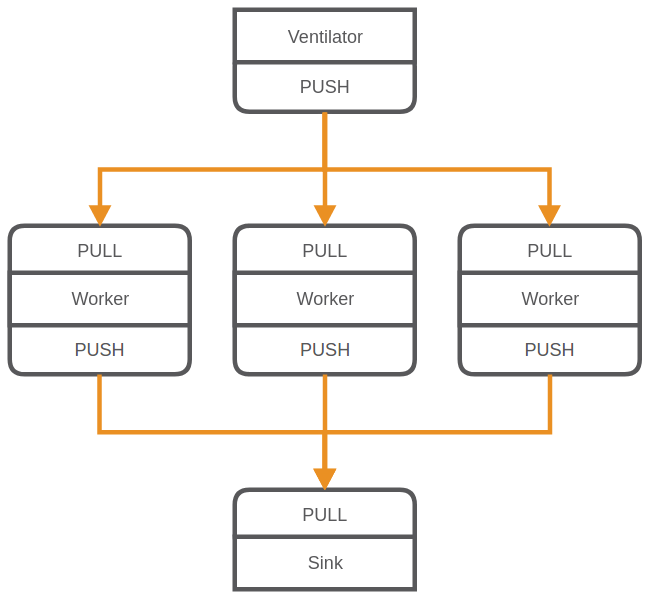
\includegraphics[width=0.6\textwidth]{resources/images/zeromq-vernitlator.png}
    \caption[ZeroMQ Pipeline architecture]{ZeroMQ Pipeline architecture. Adapted from: \autocite{ZeroMQ:Guide}}
    \label{fig:zeromq_pipeline}
\end{figure}
\textbf{Exclusive pair} connects tow sockets exclusively, for example two threads in a process.\autocite{ZeroMQ:Guide}
\newline
\textbf{Combinations of them} at least these some of the patterns in ZeroMQ.
All of these patterns can be combined to create much more advanced combinations.
Figure \ref{fig:zeromq_comination} illustrates such a combination.
\begin{figure}[H]
    \centering
    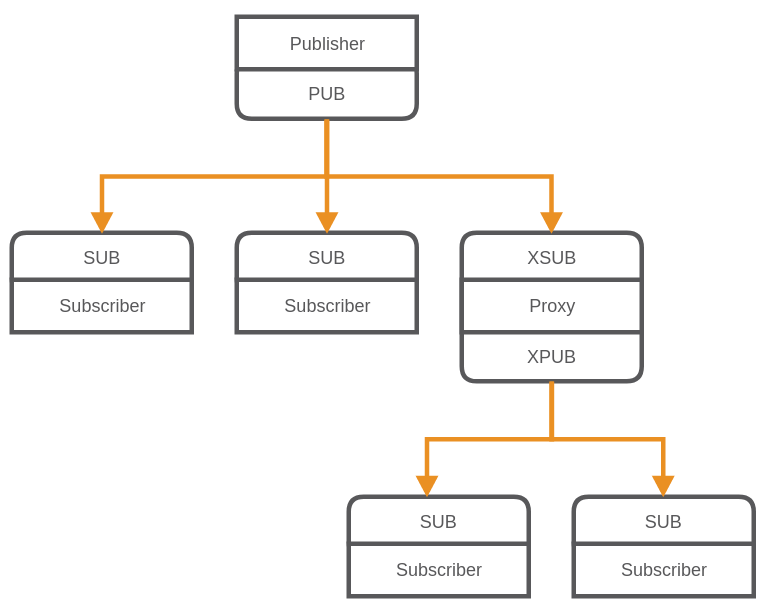
\includegraphics[width=0.6\textwidth]{resources/images/zeromq-complex.png}
    \caption[ZeroMQ combination of patterns]{ZeroMQ combination of patterns. Adapted from: \autocite{ZeroMQ:Guide}}
    \label{fig:zeromq_comination}
\end{figure}
There is a combination between two publish-subscribe patterns and a proxy in between.
This could be helpful to create a nested topology, for instances for a controller in a smart home environment.
Multiple controllers can be subscribed to a server and multiple nodes can be subscribed to one controller.
As mentioned before, there are much more combinations possible.
A good overview of many of them can be found in the official guide\footnote{\url{http://zguide.zeromq.org/page:all}} of ZeroMQ.

By default ZeroMQ has no encryption or authentication machanismn build in.
There is a dedicated project called CurveZMQ\footnote{\url{http://curvezmq.org}} which enables these functionallities and it is also created by the ZeroMQ maintainers.
Since ZeroMQ version 4.x CurveZMQ comes built-in.
Finally ZeroMQ has libraries for most of the common programming languages.

\chapter{Requirements Analysis}
\label{chapter:requirements-analysis}
\minitoc\vspace{.5cm}
Based on the fundamentals, the requirements for the prototype to be developed will be formulated in this chapter.
Thereby, relevant aspects for the specific implementation will be considered.
The analysis, the creation of requirements and the commitment from all sides to these requirements are important steps to successfully realize a project, not only in the software development area.
Each step has to be discussed and approved by a representative of the \ac{FOKUS}.
Due to the fact that the prototype will be created from scratch, most of the concepts have to be created in brainstorming meetings.
An agile development process will be used to react to rapidly changing requirements.
As mentioned before a Kanban like method will be used in this project.


\section{Functional requirements}
\label{section:functional-requirements}
% virtualization
As the fundamental requirement, the prototype to be developed has to create, manage and maintain virtualized containers on a fog node.
Tools like Open Baton inherently support OpenStack as the \ac{ETSI} \ac{MANO} \ac{VIM} layer.
Most \ac{MANO} tools like Open Baton use OpenStack, which deploys virtual machines to virtualize the \acp{NF}.
This is a rock solid solution for a cloud environment.
Unfortunately, a bare-metal virtualization is most of the time not feasible on small power devices like they are used in the \ac{IoT} area.
Therefore, a much more efficient and lightweight solution, like container virtualization, should be used and handled by an orchestration engine.
The desired service, like a \ac{NF}, can be bundled in one or multiple containers and executed afterwards on the expected \ac{IoT} nodes.
Such a bundle of containers should be passed to the node as a build plan or a blueprint of the service.
The fog node engine should accept the blueprint and deploy the containers to the desired virtualization layer.
Afterwards, the lifecycle of the services should be monitored.

% constraints
The second functional requirement is the implementation of a constraint logic, which will be used to filter relevant nodes during the orchestration.
A constraint can be a functional and non-functional capability.
For example, this could be a specific hardware component, like a sensor or a ZigBee dongle, which is necessary to execute the \ac{NF} or a hardware requirement, like \ac{CPU} power, \ac{RAM} or disk space.
It could also be a non-functional constraint, for example a specific software, which has to be installed or a protocol, that can be used.
The engine should be able to manage these constraints by itself and if necessary for all adjacent nodes and should consider them while choosing a suitable node for the desired \ac{NF}.
The whole functionality should work similar to the labels in Docker Swarm.
Therefore, a Docker Swarm node can have multiple labels, which can be considered when deploying an image.
This behavior should be achieved by the fog node engine.

% lifecycle
Another important aspect is the lifecycle management of the node, the deployed services and images.
In the prototype it has to be elaborated how the lifecycle of the several components can be implemented.
An sample implementation of a node management lifecycle is shown in the OpenFog Reference Architecture for Fog Computing\autocite[cf.][p. 52 f.]{OpenFog:2017}.
Figure \ref{fig:open_fog_node_mgm_lifecycle} describes the five steps of a typical lifecycle based on these architecture.
\begin{figure}[H]
    \centering
    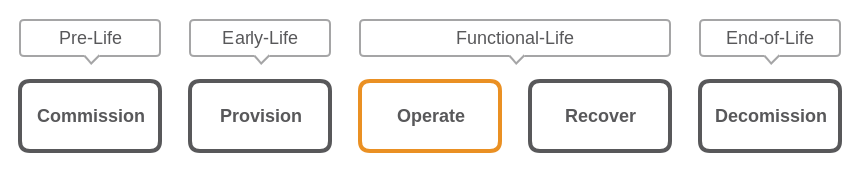
\includegraphics[width=\textwidth]{resources/images/node_management_lifecycle.png}
    \caption[Node management lifecycle]{Node management lifecycle. Adapted from: \autocite[p. 52]{OpenFog:2017}}
    \label{fig:open_fog_node_mgm_lifecycle}
\end{figure}

\begin{itemize}
  \item The \textbf{Commission} is the earliest phase in a lifecycle mostly used to perform action like identification, certificates or calibration of time.\autocite[cf.][p. 52 f.]{OpenFog:2017}
  \item In the \textbf{Provision} phase the node will be enrolled to the system so that the node can be discovered and identified and also advertises features and capabilities.\autocite[cf.][p. 52 f.]{OpenFog:2017}
  \item The \textbf{Operate} phase is the state of the node when everything operates normal.
  This includes the reliability, availability and serviceability of the node.\autocite[cf.][p. 53]{OpenFog:2017}
  \item In contrast to that the \textbf{Recover} phase performs action if something operates out of norm.\autocite[cf.][p. 53]{OpenFog:2017}
  The node should be able to recover to the normal state.\autocite[cf.][p. 53]{OpenFog:2017}
  \item Finally the \textbf{Decomission} phase is used for cleaning up sensitive data on the node and to unregister from other components.\autocite[cf.][p. 53]{OpenFog:2017}
\end{itemize}

In addition to the node lifecycle, an exemplary lifecycle for services and images is shown in the \ac{ETSI} \ac{MANO} specification\autocite[cf.][p. 67 ff.]{ETSI:MANO:2014}
This lifecycle handles several state from the instantiation of a service, further querying some data, up to the termination of service.
Some of the specifications are tightly coupled to \acp{NFV}.
However, this lifecycle specification is a good starting point to elaborate a custom solution.

% GUI
The last functional component to be developed will be the \ac{GUI}.
This should only be used to demonstrate the basic functionalities of the prototype.
It is not designed to use it in production.
Therefore, the \ac{GUI} will not have any security mechanisms like authorization, authentication or user management.
This includes that existing nodes will be displayed with all the related services.
Additionally, it can be used to deploy new services while using the existing endpoints.

% secondary conditions
Some secondary conditions should also be fulfilled.
The whole system should be modular and easy to extend.
Modules should be as decoupled as possible and the whole system should be controlled via an \ac{API}.
The centralized cloud environment should be easily replaceable and should not be exclusively bound to Open Baton or any other tool.
It also applies to the prototype, it should not be bound to Docker only and should be able to use other virtualization tools.
Finally, the whole system should be well tested and documented.


\section{Non-Functional requirements}
\label{section:non-functional-requirements}
The non-functional requirements are also addressed and they are classified into the following categories:

\paragraph{Reliability:} Due to the fact that the final product will only be a prototype and has only a few development iterations, it will not be production ready. Nevertheless the prototype will be developed with stability and robustness in mind and the code will be well tested and documented.
\paragraph{Performance:} As a crucial requirement, extra attention will be payed for making the application as lightweight as possible and reduce the dependencies and tool chain.
The use of powerful but resource consuming tools and libraries, like huge databases or message queues, will be renounced.
Necessary libraries will be used if they are essential, but in general they will be selected with the requirement of being executed on low power devices.
\paragraph{Usability:} The prototype should be easy to use, to install and to maintain.
An easy to use installation script will be developed.
The source code will be well documented and an user guide will be created.
\paragraph{Maintainability:} Due to the fact that the prototype will be a solid base for further development, it will be created as modular as possible.
It should also be well structured by using well known design patterns.
Each component should be easy to replace and also easy to maintain.
The project should be open source and extensible by everyone.
Code tests and code style checks will help to ensure the functionality and extensibility of the application.
\paragraph{Security:} Also an important part as in nearly every project, security will be considered.
Especially in the \ac{IoT} security becomes important due to several bad examples in the last years\footnote{\url{https://www.corero.com/resources/ddos-attack-types/mirai-botnet-ddos-attack.html}}\footnote{\url{https://security.radware.com/ddos-threats-attacks/brickerbot-pdos-back-with-vengeance}}.
Therefore, particular scenarios will be considered and recommendations will be addressed.
The focus of the prototype will be on showing up the functionality of the application, without implementing security related mechanisms right down to the latest detail.
\paragraph{Correctness:} As mentioned before the code will be tested and code style checks will help to have a standardized code base.
\paragraph{Flexibility:} The software will be developed with some well known standards in mind, like the \ac{MANO} specification, standard protocols and also design patterns, to make the source code more readable and understandable.
This makes it easier to add new or replace existing components.
\paragraph{Scalability:} The prototype will also be developed to be executed on several nodes at the same time.
Primary usage will be in a cluster with several other nodes.
This need will be considered during the whole development phase.


\section{Use-Case-Analysis}
\label{section:use-case-analysis}
This analysis will show up four exemplary use cases of the prototype to be developed.
These use cases describe the system in a simplified and abstract manner.
They will not refer to any technology, but will show up the usage of the prototype from a user perspective.

\paragraph{Service deployment from a cloud orchestrator:}
It will be the most common use case in this consideration.
A service, for example a \ac{NF}, should be deployed to a single node.
Figure \ref{fig:use_case_deploy_service} illustrates this use case.
Therefore, the prototype will be installed on the node itself.
A cloud service, such as Open Baton, will orchestrate the deployment.
In doing so, a so called blueprint, which is basically a description of the service, the images and the capabilities that are necessary to execute the image, will be passed over to the prototype via an \ac{API}.
The prototype will receive and parse them afterwards.
All the provided images will be executed on the same node and at the end the service is up and running.
The state of the services can be observed at any step of the process.

\begin{figure}[H]
    \centering
    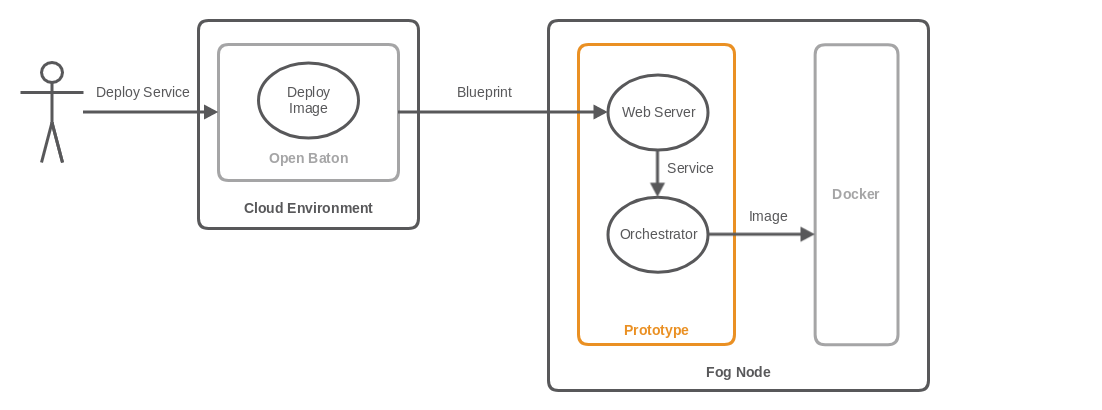
\includegraphics[width=\textwidth]{resources/images/use_case_deploy_service.png}
    \caption[Use case: Service deployment from a cloud orchestrator]{Use case: Service deployment from a cloud orchestrator}
    \label{fig:use_case_deploy_service}
\end{figure}

\paragraph{Service deployment based on capabilities:}
Also in this case a cloud service like Open Baton will deploy a service to a node cluster.
Figure \ref{fig:use_case_deploy_service_multiple_nodes} illustrates this use case.
Again, one node will get the blueprint and parse it.
Each image has labels, hereinafter called \textit{capabilities}, attached to it.
During the parsing of the blueprint, the application is checking, if the node can fulfill all of these \textit{capabilities}.
If an image can not used by this node, the application will search for a node, that is able to deploy the image.
For example, if one image needs a ZigBee dongle to measure data, than the capability \textit{ZigBee} is added to the image in the blueprint.
The first node, Node A, has no ZigBee dongle connected and therefore, it is not able to fulfill that requirement.
Node A will then ask all the other nodes in the cluster, if they can satisfy the need.
Node B will respond that it is also not able to do so.
Node C is able and will respond with a related message.
Node A sends over the image to be deployed and Node C will execute it.
From that point on, Node A is still responsible for the whole service, but Node C is executing the container that was started from the image and will frequently be asked for the state of the container.
This process can be repeated for one or multiple images.
If each image was deployed, the service is up and running and can be observed again by the user.

\begin{figure}[H]
    \centering
    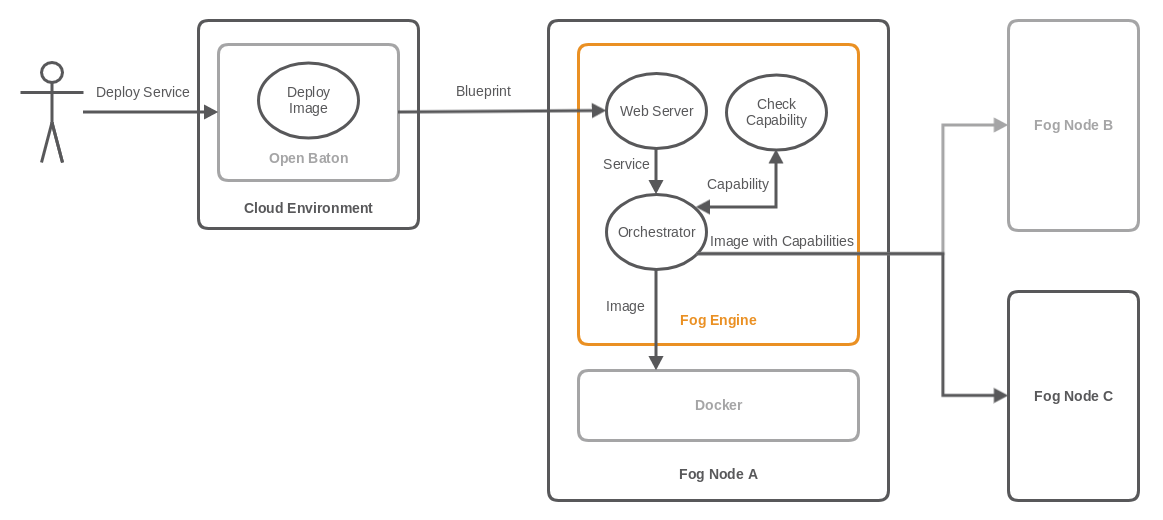
\includegraphics[width=\textwidth]{resources/images/use_case_deploy_service_multiple_nodes.png}
    \caption[Use case: Service deployment based on capabilities]{Use case: Service deployment based on capabilities}
    \label{fig:use_case_deploy_service_multiple_nodes}
\end{figure}

\paragraph{A new node will appear:}
If a new node will be added to the cluster, all the other nodes should be informed about this circumstance.
Therefore, the appearing node will send out a message with some meta information to the broker, with for example the \ac{IP} address of the node, that send it to all the other nodes.
Each node in the cluster will get the message and can store the information.
Additionally, the nodes will also send back a message with their meta information.
Again, each node will receive this message, including the newly added node.
The new node can also store the information of the other nodes.
From now on, all the nodes know each other and can directly communicate with each other.
A centralized entity is no longer necessary.
The deregistration of a node will be similar to the registration process.
The disappearing node will send out a message with meta information to all the other nodes.
They will receive them and remove the node from the local storage.
This disappeared node will no longer be part of the cluster.

\paragraph{Lifecycle management:}
The lifecycle management is important for the maintainer of the nodes.
Each process and each task in the system should be transparently and comprehensibly.
Therefore, the different components should expose their lifecycle state if requested.
The first one is the node lifecycle.
This represents the current state of the node.
Depending from the state, a node can be able to deploy a service or not.
When it is assumed, that the node is currently setting up all the necessary configurations and tools, it will then be in the state of the \textit{configuration phase}.
In this state a deployment will not be possible.
Similar to that, also the services and images will be have a lifecycle.
When a service is deployed, but does not have started all the related images, it will be in the state of \textit{instantiating} the service.
If there occurs an error while starting a container, the image and also the related service will be marked as \textit{Error} and the deployment will fail.
All of these states should also be viewable by a centralized instance like the maintainer.


\section{Delineation from existing solutions}
\label{section:delineation-from-existing-solutions}
This section is intended to show the features of existing tools and framework to highlight the main differences to the application to be developed.
As mentioned before, the intended prototype should orchestrate virtualized containers on nodes based on functional and non-functional constraints.
Therefore, the focus of this consideration is the orchestration as well as the constraints.

\paragraph{Kubernetes} is especially made for Docker and can orchestrate, scale and manage containers.
It is open source, developed by Google and one of the most popular orchestration tools on the market.
It has an active community and is used by several well known companies\autocite{Kubernetes:Case-Studies} like eBay\footnote{\url{http://www.ebay.com}} and Wikimedia\footnote{\url{https://www.wikimedia.org}}.
Due to the fact, that it is exclusively made for Docker, it means that the system is not made to switch easily the underlying container engine if needed.
The prototype will fill this gap.
It will be developed to be able to execute multiple virtualization methods.
An abstract virtualization layer is planed to be added for that need.
This makes the system more fleible and extandable for further virtualization methods.

As mentioned in section \ref{subsection:state-of-the-art:kubernetes} Kubernetes supports labels.
These are simple key-value pairs provided as \ac{JSON} objects which can be added by the system administrator to a Kubernetes Object like a pod or a service.
The labels are stored on the Kubernetes Master and can be used to filter specific pods or services during the deployment phase.
This behavior is pretty close to the one which should be achieved in the prototype.

Kubernetes is made for the cloud, which means it is not intended to be used on low power devices.
There are some attempts\autocite{kubernetes-installer-rpi}\autocite{kubernetes-on-arm}\autocite{hypriot:kubernetes-on-rpi} to do so, but until now there is no official solution for that.
The prototype will be developed with the needs of an \ac{IoT} environment in mind.
It will be executable on low power devices and pay attention for lightweight communication prototcols.
Furthermore, Kubernetes is not \ac{ETSI} \ac{MANO} compliant, but provides an easy to use web \ac{UI}.

\paragraph{Docker Swarm} is pretty similar to Kubernetes from a functional point of view.
It is open source, has an active community and it is also made exclusively for Docker.
As mentioned before, this disadvantage will be eliminated by the prototype.
The biggest benefit compared to Kubernetes is, that it is natively included in the Docker Engine.
No separate installation is necessary and it can be used out of the box.

Also in terms of labels, both platforms are similar.
Docker Swarm uses labels in the same way as Kubernetes.
The user can add them during the initialization phase or edit them during runtime.
They are also key-value pairs or alternatively keys only.
By default, labels can not be predefined in a \ac{JSON} file and applied to the node afterwards.
The placement have to be done manually via the Docker client or the \ac{REST} \ac{API}.
Labels, or so called capabilities, can be more sophisticated in the prototype and can be added into the deployment schema of a service.
This makes the system more flexible and allows deployments to handle concrete needs.

Just as Kubernetes, Docker Swarm is not \ac{ETSI} \ac{MANO} compliant and provides no build-in \ac{GUI}.
There are several third party \acp{GUI} that fix that issue, but this implies an additional setup and maintenance effort.
Due to the fact that Docker Swarm is a build-in function of Docker, the setup is quite easy and much more lightweight than Kubernetes.
This means it will also work on \ac{IoT} devices by default.

\paragraph{OpenStack} is natively supported by Open Baton and will be used by default as the underlying virtualization tool.
It only supports \acp{VM} and is mainly designed to be used in a cloud environment as well.
The installation processes is much more complex compared to Docker Swarm or Kubernetes.
There are much more dependencies and configurations to be made.

Beside the setup effort, it is an well known and established tool for \acp{NFV}, it has an active community and it is elaborated.
Compared to other tools, it is not flexible and lightweight enough for the usage in an \ac{IoT} context or more specific for the use directly on the nodes itself.
There are some efforts to move OpenStack over to the \ac{IoT} infrastructure\autocite{OpenStack:IoT}\autocite{OpenStack:Kubernetes:IoT}, but also in these attempts it will only be used in the cloud level.
Also compared to OpenStack, the prototype will have advantages to be used in an \ac{IoT} environment.
It has made to be executed on low power devices and has the same flexibility as OpenStack by switching the underlying virtualization engine.

\paragraph{Cloudify} is completely compatible to the \ac{ETSI} \ac{MANO} standard and can be used as the \ac{NFVO}, as well as the generic \ac{VNFM} of this architecture.\autocite[cf.]{Cloudify:MANO}
It is also able to interact with multiple \acp{VIM}, containers, infrastructures and devices and due to the fact that it can be extended with plugins, it can be used together with several well known tools like OpenStack, Docker or even Kubernetes.\autocite[cf.]{Cloudify:MANO}
Because of this flexibility, Cloudify can also be used in an \ac{IoT} environment if an appropriate \acp{VIM} plugin is used.
Downside is, that Cloudify itself needs an orchestration tool like OpenStack to be used as \ac{NFVO}.
Without an underlying orchestration tool it is limited.

By default it is also not possible to orchestrate functionalities based on constraints.
To enable this behavior the used plugin has to support such a functionality like Docker Swarm or Kubernetes.
Cloudify provides an easy to use \ac{GUI}, so that the user can manage the whole system, as well as a clean command line tool.
By using the \ac{YAML} format to build service blueprints, the creation of them is similar to well known Ansible or Vagrant deployment schemes.
With the help of the Cloudify Composer the creation of a blueprint is getting much easier and also usable for users without any coding experience.

Due to the fact that the prototype will have a \ac{REST} \ac{API}, it could be possibly be integrated into Cloudfiy with a minimal development effort.
Beside that, it can enrich some of the Cloudify functionalities, for example by adding the capability behavior or an inter-node communication.

% https://www.sdxcentral.com/products/gigaspace-cloudify/

\acresetall

\chapter{Concept}\label{chapter:concept}
% This chapter introduces the architectural design of Component X. The component consists
% of subcomponent A, B and C.
% In the end of this chapter you should write a specification for your solution, including
% interfaces, protocols and parameters.
This chapter introduces the architectural design of plugin respect to the previously defined requirements.
Therefore the used development environment will be analyzed.
Followed by the initial architecture of the plugin to be developed.
Based on that the different layer of the system will be elaborated.

\section{Overview}
% The concept chapter provides a high-level explanation of your solution. Try to explain
% the overall structure with a picture. You can also use UML sequence diagrams for
% explanation.
% Figure 4.1 illustrates the situation between Alice and Bob. (sequence diagram from
% www.websequencediagrams.com)
\doit

% Docker Plugin as Vim Driver

\section{Development environment}
The development environment is crucial for both the implementation of the prototype, as well as the choice of possible plugins and libraries.
It should be easy to used and fast to implement, but it should also consider the knowledge of the \ac{FOKUS} as well as the developer.

\textbf{Java } is still one of the most important programming languages out there.\autocite[cf.]{ProgramminLanguage:2017}
Java is platform indipendent, because Java will not be executed directly in the \ac{OS}, instead it will be executed in the \ac{JVM}.
The downside is, that especially because of the \ac{JVM}, Java programms are much more inefficient regarding \ac{RAM} and \ac{CPU} usage.
Java is object oriented, which makes it easy to extend.
There are a lot of well designed and developed establised libraries and tools out there, which makes it easy to create rapid prototypes.

\textbf{Python:} is one of the most used programming languages with a huge and active community.\autocite[cf.]{ProgramminLanguage:2017}
\todo{write something}


\textbf{Node.js:} is a relativly young programming environment, which was created 2009 by Ryan Dahl and based on the Google JavaScript engine V8.
The V8 engine is written in C++, which makes the language less resources consuming then for example Java.
A programm will be written in JavaScript, but it is also possible to load C or C++ extension.
Node.js is also available for all common \acp{OS}.
Due to the fact that Node.js has a build-in webserver componant, it is easy to create web applications.
Libraries can be added via the package manager called npm.
JavaScript and also Node.js have a pretty active community, which tends to be as messy as they is increasing.
There is enormous amount of libraries and tools out there, where each library has its reason to exist, but it is also a vast of pretty similar designs and use-cases.

\textbf{Go:} is the new emerging language created by Google and was announced end of 2009.
It follows the traditions of C, but also takes added concepts to create a more modern programming language.
According to their own statements go is expressive, concise, clean, and efficient.\autocite[cf.]{Go:Documentation}
Furthermore it has a garbage collection and run-time reflection, it is fast, statically typed and a compiled language.\autocite[cf.]{Go:Documentation}
Go is used in production by several tools like Docker, Kubernetes and OpenShift.
Downside is that there are not so much libraries out right now and there are no long time experience in the critical mass.

Open Baton, as one of the actively maintained project at the \ac{FOKUS}, is written in Java and is also has ports to python and go.
Python in general is used for several projects at the \ac{FOKUS}.
Taking also the criterias from section \ref{section:technical-requirements} into account python will be used as the  programming environments of choice.
The \ac{GUI} will only be a very basic web client, which uses Vue.js\footnote{\url{https://vuejs.org}} as its main framework and some smaller tools like the pretty famous bootstrap framework.

\section{Architecture of the system}
The overall architecture of the system can be seperated into two levels.
Figure \ref{fig:abstract_architecture_design} will point up the architecture.
The first level is the \textit{centralized fog level}.
This could be for example a cloud server or management node in a fog cluster.
Ideally this level should be implemented with an \ac{MANO} compliant framework.
Hereinafter Open Baton will referred as the tool of choice for that level.
Main function will be the creation of the \ac{NFVI} as well as the deployment of deployment plans for the \acp{NF}.
Open Baton will also have an overview of all existing nodes and can manage and maintain them.

\begin{figure}[H]
    \centering
    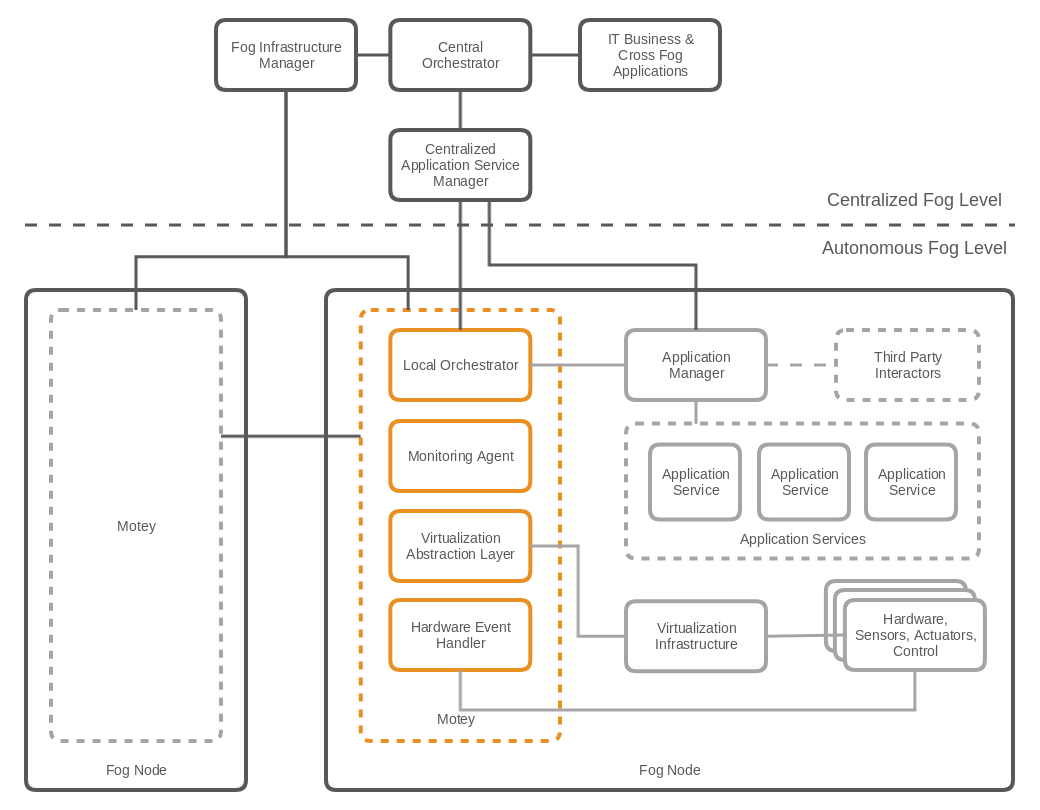
\includegraphics[width=\textwidth]{resources/images/initial_structure.png}
    \caption[Abstract architecture design]{Abstract architecture design}
    \label{fig:abstract_architecture_design}
\end{figure}
% TODO: check if applicaton manager is necessary

The second level is the \textit{autonomous fog level}.
The prototype to be developed will be located in this level.
It includes all existing fog nodes, as well as the prototype referenced as the \textit{OpenIoTFog Agent} in figure \ref{fig:abstract_architecture_design}.
Each node must have a running instance of the OpenIoTFog Agent to be part of the system.
Beside the prototype a node can have several hardware devices, sensors and actuators connected to them.
A virtualization infrastructure such as Docker or XEN, must be installed to be used by the prototype.
These infrastructure can create the containers and \acp{VNF}.
Further it is also possible to have additional third party tools installed which can interact with the them as well.

The OpenIoTFog Agent has several external connection points.
It has a \ac{REST} \ac{API} implemented to get some informations about the status of the fog node, as well as endpoints to receive the deployment plans from centralized fog level.
A \ac{MQTT} connection to a broker, which can be running in the centralized fog level as well as on any other fog node, is used for node discovery.
Finally there are some ZeroMQ endpoints for capability discovery, image deployment and node-to-node communication.
A detailed description will be shown in the following sections.

One of the most important components is the \textit{Local Orchestrator}.
It is responsoible for the deployment of the containers as well as the inter-node communication.
The latter is necessary to let the nodes act in an autonomously was, so that they can react to changing requirements, even when the centralized fog level disappears.
Therefore each node must have knowledge and should be able to interact with each other.
Beside that the local orchestrator is tightly coupled to the \textit{\ac{VAL} Manager}.
This is an abstraction layer for each virtualization component in the system, for example Docker or a bare-metal virtualization like XEN.
These components should be implemented as plugins, so that it is easy to add or remove virtualization components.
Therefore Yapsy\footnote{\url{http://yapsy.sourceforge.net/}} is used as the plugin system of choice.

The \textit{Hardware Event Handler} is a communication endpoint for other third party components.
For example an external hardware listener could send a message to the event handler to register a new connected device like a Zigbee dongle or a bluetooth stick.
This component should allow multiple third party components to send events to them.
Finally the \textit{Monitoring Agenct} is used to log all ongoing events and gives the maintainer of the system an overview of the system processes.
\todo{write more - probabyl about architecture MVC}
% MVC ohne View
% -> keine spezielle architektur
% -> jedoch decoupled as much as possible
% ---> DI, RxPy

\subsection{Virtualization layer}
The virtualization layer is basically an abstraction layer to generalize the different virtualization engines.
Therefore a so called \ac{VAL} manager which will be implemented with the facade design pattern is used to load the plugins and abstract the methods of the plugins.
As mentioned before to realize the plugin functionality the Yapsy library will be used.
The library offers a way to easily add new plugins to the system and is also designed to be easy to use.
It only depends on python standard libraries and lightweight by design.
Each supported virtualization engine needs his own concrete plugin implementation which should be use an interface to have a common ground.
The supported default engine is Docker, but could be extended in a future version of the prototype.

\subsection{Communication layer}
\label{subsection:CommunicationLayer}
The communication layer is a pretty important componant in the prototype.
Here three different communication points are necessary to provide the basic functionalities which are needed for the fog node agent.

The first subcomponent is the \textbf{node discovery}.
The idea behind the node discovery is that each node automatically can register and unregister himself to the cluster.
This means in the moment of the startup of a node, they will send out a message, with an information request about all subscribed nodes.
To realize that \ac{MQTT} will be the tool of choice.
The \ac{MQTT} broker will receive and forward the message to all subscribed nodes and each node will response with an information message to the broker again, which will send the message out again.
Therefore each node will be up-to-date at each time.
As long as there is no appearance or disappearance of any node, the network will not be stressed.
To provide a better flexibility the \ac{MQTT} broker can be executed in the centralized fog level or even on a node in the autonomous fog level.
This allows the system to operate even if the centralized fog level disappears due to network issues or any other communication problems.
It is also possible to let all nodes communicate which each other once they shared their information.
Smaller connection issues can be covered with this mechanism.
As the \ac{MQTT} broker Mosquitto\footnote{\url{https://mosquitto.org}} will be the tool of choice.
It is an eclipse\footnote{\url{http://www.eclipse.org}} project which means it is open source and under continous development.
The project website descibes themself as "a lightweight server implementation of the MQTT protocol that is suitable for all situations from full power machines to embedded and low power machines"\autocite{Eclipse:Mosquitto}.

The next subcomponent is the \textbf{inter- and intra-node communication}.
Both kinds of communication will be realised with ZeroMQ.
Some of the most important patterns and transport types in ZeroMQ was discribed in section \ref{section:ZeroMQ}.
For the node-to-node communication the \textit{Request-Reply} pattern via \ac{TCP} will be used.
Typical function calls would be the capability discovery where a node will request another node for their capabilities, the deployment or termination of an image on an external node and the request for an image status.
ZeroMQ allways requires an \ac{IP} to eastablish a connection to another node, therefore we had the node discovery which was described before.
This allows us to connect to any other node in the cluster.
In addition to the intra-node communication, also an inter-node communication will be implemented.
It will be used to add new capabilities to a node.
Therefore one or multiple third party applications should be connectable to a single ZeroMQ endpoint via the publish/subscribe pattern over \ac{IPC}.
Different to a normal publish/subscribe pattern, the endpoint will acts as the subscriber so that multiple publishers can push messages to them.
Beside that each exposed socket should be configurable via the configuration file.

The last subcomponent is the \textbf{\ac{REST} \ac{API}}.
It will be mainly used for the communication with the centralized fog level, because most of the orchestration tools out there are using \ac{REST} for transfering data.
In comparision to an implementation with ZeroMQ, this is much bigger overhead in terms of traffic and latency, but to have a better compatibility with other systems, this \ac{API} will be implemented.
As the tool of choice Flask\footnote{\url{http://flask.pocoo.org}} will be used.
It is a lightweight and robust python webserver, which is open source, well documented and under constant development.
The \ac{REST} \ac{API} himself will follow the \ac{HATEOAS} constraint with the addition that each endpoint will have a version number in the \ac{URL} to ensure backwards compatability if something changes in the implementation.

All the mentioned subcomponents should be controlled by a so called \textit{communication manager} which will be implemented with the facade design pattern.
That decouples the communiction layer from the other components, the whole system can be maintained much easier and each subcomponent can be easy replaced by any other technology if necessary.
This also makes the code more readable and leads up to a cleaner code strucutre.

\subsection{Data layer}
As mostly the data layer is used to persist necessary data.
This includes the deployed services, adjacent nodes and the capabilities of the node.
As database engine the lightweight document oriented database TinyDB\footnote{\url{http://tinydb.readthedocs.io}} will be used.
It stores the data into a single \ac{JSON} file, which means it has only very basic functionalities.
For example it does not support indexes or relationships and it is not optimised concerning performance.
But for it is easy to use, has no execution overhead and is good to use for small datasets.
The whole data layer should be as abstracted as all the other components before.
Therefore repositories for each content type will facade the tinydb methods and allows the underlaying library, in this case TinyDB, to be replaced easily and
without modifing several classes.
The configuration of the databases should be stored in the global config file as well.

\subsection{Capability Management}
The \textit{Capability Management} is used to create, persist, modify and remove the capabilities of the current node.
As mentioned before all the capabilities will be stored in the data layer via TinyDB.
Furthermore the \textit{Hardware Event Handler} is part of this layer.
It enables the system to get new capabilites from third party apps via a ZeroMQ endpoint.
As mentioned in the \ref{subsection:CommunicationLayer} the endpoint will be implemented as a form of the publish/subscribe pattern and should allow one or multiple publishers to push messages to the handler.
Also internal components like the \ac{VAL} plugins can add new capabilities to the system.

\subsection{Orchestration layer}
% ist primär für das Blueprint handling zuständig
% -> bekommt daten via api und parst diese
% -> guckt ob lokal deployed werden kann oder externe Node benötigt wird
% -> yaml als blueprint format
% sowie für die node-to-node Kommunikation
% -> Nodes registrieren sich beim starten der Engine
% -> können capabilities erfragen
% -> können container starten
% -> Sequenzdiagramme für die unterschiedlichen fälle erstellen
\doit

\subsection{User interface}
\doit

\subsection{Security}
% Access control
% Encryption of the communcation channels aka REST, ZeroMQ, MQTT
\doit

\subsection{Continuous Integration}
Continuous integration is nowadays a frequently used technique to automate repeating deployment steps into a self executing pipeline.
It starts by running unit tests, code style checks and ends up with deploying the compiled programm to a server or a marktplace.
Due to the fact that Github\footnote{\url{https://github.com}} will be used to host and maintain the git repository for the prototype, the pretty famous and semless integrated Travis CI\footnote{\url{https://travis-ci.org}} will be used to implement the continuous integration pipeline.
To start with Travis CI only the Github account has to be synced with the platform and a \ac{YAML} configuration file has to be placed in the root folder of the git repository.
Travis CI supports several programming languages and also various third party services, like Docker Hub or Amazon AWS.
Everytime a new commit will be pushed to the git remote repository, a new build will be started at Travis CI.
At first a virtual machine will be started by Travis CI.
Afterwards all necessary components like libraries and tools will be installed in the virtual machine.
Finally all predefined tasks from the \ac{YAML} file will be executed.
In terms of the prototype, unit tests will be executed, as well as code style checks and if a version from the master branch will be build, a Docker container will be created and pushed to the related Docker Hub repository.
This pipeline guarantees that the project is tested and a coding standard is enforced.
Further the manual build of the Docker container including the upload to the Docker Hub will be obsolete.

\section{Conclusion}
\doit



% http://getcloudify.org/brochures/Heavy%20Reading%20NFV%20MANO%20Cloudify%20Snapshot.pdf

\chapter{Implementation}
\label{chapter:implementation}
\minitoc\vspace{.5cm}
This chapter describes the implementation of the Motey engine as well as the deployment and capability logic.
Used technologies, libraries and tools, as well as custom components would be presented and the functionality will be demonstrated.
Thereby challenges and problems during the development of the plugins will be shown and the solutions will be discussed.

\section{Environment}
To Motey engine is designed to be executed on low-power devices like a Raspberry Pi.
The following software is required to execute the whole software stack.
\begin{itemize}
  \item Ubuntu version 14.10 or higher
  \item Python 3.5 or newer
  \item Docker 17.3 or higher
\end{itemize}
On hardware side Motey will be tested on Raspberry Pis type 2 B or newer.
Depending on the amount and type of the executed Docker images, the hardware specifications may can vary.


\section{Project structure}
Beside the main folder with the Motey engine, the project contains several directories with helpful scripts and tools.
A brief overview about the project structure will given in this section.
A detailed explanation of all files will be omitted, as this would exceed the scope of the thesis.

\begin{itemize}
  \item{\textbf{Directory: ./}} has all the necessary configuration files for the different services.
  \begin{itemize}
    \item{\textbf{File: .dockerignore}} is used during the build process of a Docker image. Excludes several folders during the build phase.
    \item{\textbf{File: .editorconfig}} contains information for \acp{IDE} and editors to guarantee a consistent coding style.
    \item{\textbf{File: .gitignore}} excludes file to be tracked by the version control system git.
    \item{\textbf{File: .travis.yml}} is used by the continuous integration tool Travis CI.
    \item{\textbf{File: AUTHORS.rst}} a list of all contributors.
    \item{\textbf{File: CHANGELOG.rst}} this document records all notable changes to the Motey engine.
    \item{\textbf{File: LICENSE}} the License of the project (Apache License Version 2.0).
    \item{\textbf{File: main.py}} can be used to start Motey in debug mode.
    \item{\textbf{File: MANIFEST.in}} contains meta information for the Python setup procedure.
    \item{\textbf{File: README.rst}} file to show up a short documentation on Github and will act as the starting point of the project.
    \item{\textbf{File: setup.py}} will be used to install Motey on a local machine.
  \end{itemize}
  \item{\textbf{docs:}} contains the files to create and display the documentation resources.
  \begin{itemize}
    \item{\textbf{Directory: source}} has all the files to auto-generate the documentation files from the source code.
    \item{\textbf{File: Makefile}} this file was created by the Sphinx documentation tool. By executing the \textit{Makefile} the related documentation files will be created.
  \end{itemize}
  \item{\textbf{motey:}} this folder contains the Motey main engine. It is the main Python project. The whole structure will be explained on the next pages in detail.
  \item{\textbf{motey-docker-image:}} has all the necessary files to create a Docker image.
  \begin{itemize}
    \item{\textbf{File: Dockerfile}} to build the Docker image. Is analogous to a Makefile but can only be used by the Docker engine.
    \item{\textbf{File: setup.sh}} will be executed during the build phase and will install necessary tools and can executed command line instructions.
    \item{\textbf{File: requirements.txt}} a list with the Python requirements which are necessary to run the Motey engine and which should be installed during the build phase via pip.
  \end{itemize}
  \item{\textbf{motey-rpi-docker-image:}} is pretty similar to the motey-docker-image directory but is specifically made for the Raspberry Pi image.
  \item{\textbf{performance\_test:}} contains scripts that are used to perform performance tests for the evalutation chapter.
  \item{\textbf{resources:}} is a resource folder for the Github documentation. Will only be used by the \textit{README.rst} file in the root folder and the \textit{index.rst} file in the docs\/source folder.
  \item{\textbf{samples:}} contains some samples to test the functionality of the Motey engine. Is primarily a playground to test new functions.
  \item{\textbf{scripts:}} some scripts which will be executed frequently during the development phase.
  \begin{itemize}
    \item{\textbf{Folder: config}} configuration files which could be used for the Mosquitto \ac{MQTT} broker Docker image.
    \item{\textbf{File: addcapability.py}} can be used to add new capability entries to a running Motey instance.
    \item{\textbf{File: start\_test\_setup.sh}} can be used to start a new local Docker test cluster.
  \end{itemize}
  \item{\textbf{tests:}} contains all the unit test which are executed by the continuous integration script and the Python setup procedure.
  \item{\textbf{webclient:}} this folder contains the \ac{GUI} for the Motey engine. Will also be described on the next pages in detail.
\end{itemize}

\section{Used external libraries}
This section will show up some of the most important libraries used in the Motey engine.
Each library will be introduced briefly and the reason for using it in the project will be shown.

\paragraph{daemonize}\label{library:daemonize} allows to run a services as a daemon process.
It is made exclusively for Unix-like systems.
The library will create a pid file after starting the service.
In the Motey engine, the file path can be configured via a configuration file.
The daemon process can be controlled via a command line interface.
\begin{listing}[H]
  \begin{minted}{shell}
  Motey command line tool.

  Usage:
    motey start
    motey stop
    motey restart
    motey -h | --help
    motey --version

   Options:
     -h, --help       Show this message.
     --version        Print the version.
  \end{minted}
  \caption{Command line interface documentation for the daemon process}
  \label{code:cli-tool}
\end{listing}
After the Motey engine is installed via the setup script, this command line tool will be available in the terminal.

\paragraph{dependency-injector} is a microframework for \acf{DI} in Python.
The \ac{DI} pattern allows to move the responsibility for creating a dependency from the concrete objects to a factory or a framework which creates the dependency graph.
This grants the single responsibility concept for classes and makes the whole code base much easier to unit test, because a dummy object can be passed to the constructor of the class.
It is also possible to mocked the object with the help of a mocking library.
To realize \ac{DI} in the Motey a so called \textit{app\_module.py} was created which uses the \textit{dependency-injector} framework to create the dependency graph.
Several \ac{IoC} containers are created in that file and will be used by the framework to generate the glue code.
Most of the injected components are instantiated as singleton objects to guarantee that there is only one active instance of that component at a time.
The implementation of the singleton design pattern is also provided by the framework.
Listing \ref{code:app-module} demonstrates the implementation of such an \ac{IoC} container.
\begin{listing}[H]
  \begin{minted}{python}
  class DIRepositories(containers.DeclarativeContainer):
      capability_repository = providers.Singleton(CapabilityRepository)
      nodes_repository = providers.Singleton(NodesRepository)
      service_repository = providers.Singleton(ServiceRepository)
  \end{minted}
  \caption{Extract of a sample \ac{IoC} container from the app\_module.py}
  \label{code:app-module}
\end{listing}

\paragraph{Docker \ac{SDK}}
The Docker Python library is a wrapper around the Docker command line tool.
Every command that can be executed with this tool can also be executed from any python code.
In the initializing phase the library will connect to the Docker Engine \ac{API} and will perform all the actions through them.
This can be realized via an \ac{URL} to the \ac{REST} \ac{API} or via an Unix system socket connection.
In the Motey engine the second method will be used, but can be replaced without any limitations.
The library is used as a \ac{VAL} plugin and will be automatically loaded at runtime via the VALManager and the Yapsy plugin system.

\paragraph{Flask} is a framework to create web applications.
Flask does not provide any templating or database engine, nor does it enforce a specific file structure.
Instead it will support extensions to add functionalities like that so that the developer can choose the tools of choice.\autocite[cf.]{Flask:Documentation:Foreword}
Nevertheless Flask is production ready and is used in several big projects like Pinterest\autocite{Quora:Pinterest:Flask} or Twilio\autocite{Twilio:Flask}.

Flask can use so called \textit{Blueprint} to configure new routes in the webserver.
A Blueprint is basically a Python class that can define methods like \textit{get} or \textit{post} to handle the specific \ac{HTTP} verbs.
This is useful to create valid \ac{HATEOAS} \ac{REST} \acp{API}.
Each Blueprint will be represented by an \ac{URL} endpoint.

Listing \ref{code:flask-blueprint} illustrates the implementation of all \ac{API} endpoints in Motey.
\begin{listing}[H]
  \begin{minted}{python}
    def configure_url(self):
      self.webserver.add_url_rule('/v1/capabilities', view_func=Capabilities.as_view('capabilities'))
      self.webserver.add_url_rule('/v1/nodestatus', view_func=NodeStatus.as_view('nodestatus'))
      self.webserver.add_url_rule('/v1/service', view_func=Service.as_view('service'))
      self.webserver.add_url_rule('/v1/nodes', view_func=Nodes.as_view('nodes'))
  \end{minted}
  \caption{Implementation of all Flask \ac{API} endpoints in Motey}
  \label{code:flask-blueprint}
\end{listing}

In line 2 a new endpoint will be add via the \textit{add\_url\_rule} to the Flask webserver.
The first parameter indicates the endpoint \ac{URL} and the second parameter \textit{view\_func} represents the Blueprint class, in this case \textit{Capabilities}.
To pass them over, the Blueprint has to be converted to a Flask view by using the \textit{as\_view} method.
The other endpoints are implemented equivalent.

\paragraph{Logbook} is a small logging library that helps to standardize the output of log messages.
It helps to address several output methods like the terminal, a file or even emails and Linux desktop notifications.
The style of the resulting message can be easily configured and it can be integrated into several other libraries.
In addition to that, Logbook has a build-in support for messaging libraries like ZeroMQ, RabbitMQ or Redis.
This allows to distribute log messages on heavily distributed systems like a huge node cluster.
It was created by Armin Ronacher the creator of Flask and Georg Brandl the creator of Sphinx, both are tools that are used in Motey.
Unfortunately there is no build-in support in Flask yet.
In the Motey engine Logbook will be extended by a wrapper class to simplify the configuration of the tool.
The output folder for the log messages can be configured via the global config file and will be loaded in the constructor of the wrapper class.
If the folder path does not exist, it will be created.

\paragraph{paho-mqtt} is the python implementation of the Eclipse paho\footnote{\url{http://www.eclipse.org/paho}} project that is basically the implementation of the \ac{MQTT} messaging protocols, which was already described in section \ref{section:MQTT}.
The library allows to connect to a \ac{MQTT} broker like the Mosquitto broker.
It also comes with a variety of helper methods to eases the usage.
A wrapper class to centralize the usage of the library was created and the configuration as well as some smaller improvements was made in this wrapper class.
The whole configuration of the client can be configures via the global config file again.
Furthermore the routes are managed in the wrapper and a after connect handler was implemented.
It will be used to perform actions after a successfully created connection to the broker was made and all subscriptions to topics are done.
This helps to realize the node discovery mechanism described in section \ref{subsection:CommunicationLayer}.

\paragraph{pyzmq} is the third important communication library.
It is the official Python binding for ZeroMQ.
A detailed description of ZeroMQ can be found in section \ref{section:ZeroMQ} and in the great ZeroMQ guide at \url{http://zguide.zeromq.org/page:all}.
This library is also abstracted by wrapper class in Motey.
This helps to configure the ZeroMQ server and register all necessary nodes.
A detailed explanation of the internals will be discussed in the following section \ref{subsection:implementation-communication-layer}.

\paragraph{Sphinx} is a tool to auto-generate a documentation out of the source code documentation.
It supports several output formats like \ac{HTML}, \LaTeX\ or ePub and is the de facto standard in Python.
The documentation hosting platform Read the Docs\footnote{\url{http://readthedocs.org}} completely supports Sphinx documentations.
As mentioned before the Makefile in the docs folder will be used to auto-generate the documentation files.
The scripts handles also the deployment of the documentation.
Therefore the files will be generated, the current branch will be switched to \textit{gh-pages}, which is be used to display the Github page at \url{https://neoklosch.github.io/Motey/} and a new commit will be pushed with an auto-generated commit message.
Finally the branch will be switched back again.
Read the Docs has an active webhook that builds the builds the current documentation and display them at \url{http://motey.readthedocs.io}.
The documentation is also used as the official Github page of the project at \url{https://neoklosch.github.io/Motey}.

\paragraph{TinyDB} is a wrapper to implement a lightweight document oriented database.
It stores the data into single \ac{JSON} files.
The location can be configured via the global config file.
TinyDB only supports very basic functionalities.
For example it does not support indexes or relationships and it is not optimized concerning performance.
But it is easy to use, has no execution overhead and it performs very well on smaller datasets.
The main purpose of the library is to be used for small apps where database server like MySQL\footnote{\url{https://www.mysql.com}} or MongoDB\footnote{\url{https://www.mongodb.com}} will be a huge overhead.
Furthermore TinyDB has several extension to add more functionalities like indexing or caching.
It also allows to easily extend the library with custom middlewares and extensions.
In the Motey engine, TinyDB is used in every \textit{repository} to decorate the usage of the library.
Thereby the used library can easily replaced by a different one, without refactoring several class in the project.
A detailed description of the implementation will be shown in \ref{subsection:impl-data-layer}.

\paragraph{Yapsy} is a plugin system that was designed to make an application easily extensible and should also be easy to use.
Several plugin systems are too complicated for a basic usage or have a huge dependency overhead.
Yapsy claims to be different, because it is written in pure Python and can be used with only a few lines of code.
In the Motey engine all \ac{VAL} plugins will be loaded via Yapsy.
An extract of the VALManager with the method to register the plugins, is shown in listing \ref{code:yapsy-register-plugins}.
\begin{listing}[H]
  \begin{minted}{python}
  def register_plugins(self):
    self.plugin_manager.setPluginPlaces(
      directories_list=[absolute_file_path("motey/val/plugins")]
    )
    self.plugin_manager.collectPlugins()
    for plugin in self.plugin_manager.getAllPlugins():
        plugin.plugin_object.activate()
  \end{minted}
  \caption{Extract of the VALManager with the method to register plugins}
  \label{code:yapsy-register-plugins}
\end{listing}
In Motey there is a specific folder where all images has to be located (line 2).
This could be extended in the future if necessary.
Afterwards all the valid plugins will be loaded and activated (line 3).
Finally for all activated plugins the \textit{activate} method will be executed, which is a custom implementation to call some functions after activating a plugin (line 4 and 5).
All plugins can be used via the \textit{self.plugin\_manager}.

\section{Important Implementation Aspects}
This section will introduce to the most important aspects of the implementation of the Motey engine.
At first a short overview of the whole class structure will be shown, followed by a detailed explanation of the major components.
Finally the created \ac{GUI} as well as the \ac{CI} pipeline will be explained.


\subsection{Motey engine}
% You can also compare different approaches. Example: Since the implementation based
% on X failed I choosed to implement the same aspect based on Y. The new approach
% resulted in a much faster ...
The main component in the Motey engine is the \textit{Core} class.
It will start all the necessary components to run the engine.
The core can be executed in debug mode or as a daemon.
Latter creates a pid file which can be configured via the \textit{config.ini} file.
The dependencies of the most important components is shown in figure \ref{fig:motey_class_diagram}.

\begin{figure}[H]
    \centering
    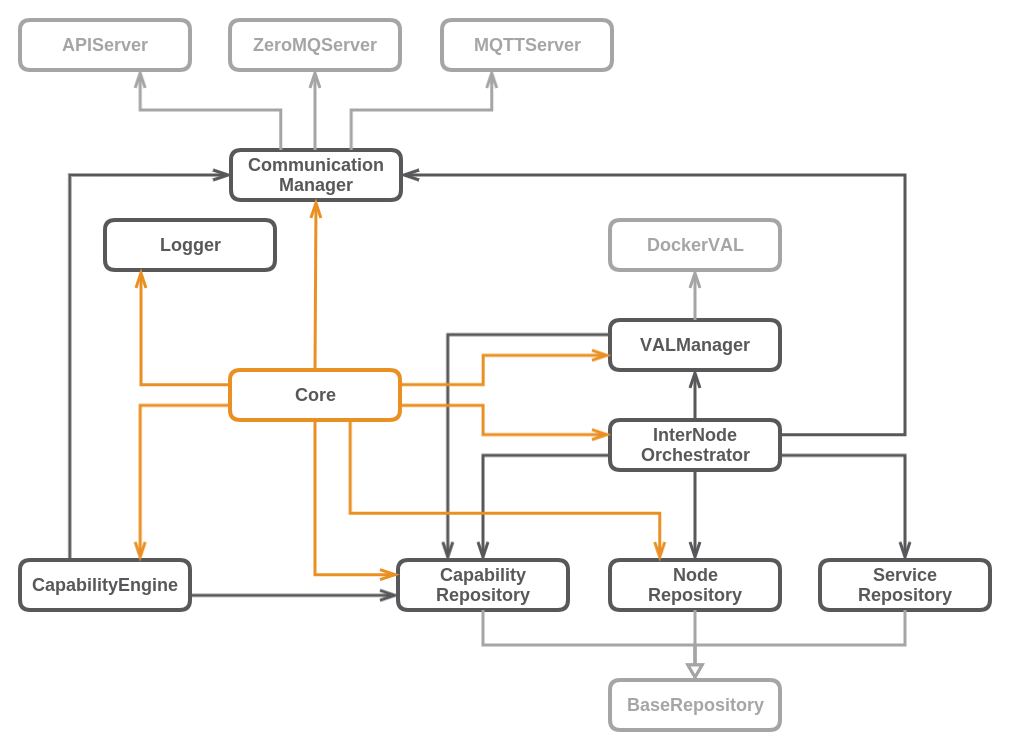
\includegraphics[width=\textwidth]{resources/images/class_diagram.png}
    \caption[Motey class diagram]{Motey class diagram}
    \label{fig:motey_class_diagram}
\end{figure}

This class diagram is simplified in a way that not all components and not all dependency connections are shown.
But it is pretty helpful to get an basic understand of the interconnection of the different layers.
A good example of the decorator pattern can be found in the top left corner of the diagram.
The \textit{CommunicationManager} acts as a decorator for all the connection endpoints.
Therefore it is easy to add a new endpoint or replace an existing one, only the \textit{CommunicationManager} has to be modified instead of all the classes which uses the communication layer.
Another example for that behavior is the \textit{VALManager}.
Also this class acts as a decorator and manages all virtualization plugins, in this case the \textit{DockerVAL}.
The repositories are a special case of the decorator pattern, because they covers the usage of the \textit{TinyDB} library, but they are also a centralized place for using them instead of all over in the engine.
The \textit{CapabilityEngine} and the \textit{InterNodeOrchestrator} are the only component that uses the \textit{CommunicationManger}.
The \textit{Core} also imports that class but only to start them.
Beside the \textit{Core} the \textit{InterNodeOrchestrator} is the central place in the app.
Each event will be executed in the layer.
Therefore most of the other components will be come together in this class.
In the following the separate layers are described in detail.


\subsection{Data layer}
\label{subsection:impl-data-layer}
As mentioned before TinyDB is used as the database engine of choice.
To abstract TinyDB from the rest of the source code, the repository pattern will be used.
Each content type has its own database and also a related repository.
All of them are inheriting from the \textit{BaseRepository}.
This repository is used to implement some default methods and will also create the database path in the constructor if it is necessary.
Beside that all of them are pretty similar implementation-wise.
They only differ in using different models and have some specific methods to be executed.
These models are used to represent the related \ac{JSON} objects.
Therefore each of them have a static transform method to convert \ac{JSON} objects to the related model.
The models folder also contains a file called \textit{schemas.py}.
This file contains the validation schemes for the different \ac{YAML} and \ac{JSON} objects that could be received by the nodes.
A library called \textit{jsonschema} is used to validate the objects based on such a schema.
An example for a schema is shown in listing \ref{code:capability-schema}.
\begin{listing}[H]
  \begin{minted}{python}
  capability_json_schema = {
      "type": "array",
      "items": {
          "type": "object",
          "properties": {
              "capability": {
                  "type": "string"
              },
              "capability_type": {
                  "type": "string"
              }
          },
          "required": ["capability", "capability_type"]
      }
  }
  \end{minted}
  \caption{Capability JSON validation schema}
  \label{code:capability-schema}
\end{listing}
The \textit{jsonschema} library allows to validate the type of an entry (line 2, 7 and 10) and also if the fields are required or optional (line 13).
This guarantees that only valid objects will be processed.

Another data layer component is the configuration reader.
This is implemented with the default Python \textit{configparser}.
The parsed configuration is only kept in memory.
The configuration file for the whole project is stored in the \textit{motey/configuration} folder and is called config.ini.
Listing \ref{code:config-ini} show the sample content of that file.
\begin{minted}{python}
[GENERAL]
app_name = Motey
pid = /var/run/motey.pid

[LOGGER]
name = Motey
log_path = /var/log/motey/
file_name = application.log

[WEBSERVER]
ip = 0.0.0.0
port = 5023

[MQTT]
ip = 172.18.0.3
port = 1883
keepalive = 60
username = neoklosch
password = neoklosch

[DATABASE]
path = /opt/Motey/motey/databases

[ZEROMQ]
capability_engine = 5090
capabilities_replier = 5091
deploy_image_replier = 5092
image_status_replier = 5093
image_terminate_replier = 5094
\end{minted}
\captionof{listing}{Example of the config.ini file\label{code:config-ini}}
\vspace{0.5cm}
Different sections can be separated by squared brackets like \textit{[GENERAL]} like on line 1.
The entries are simple key-value pairs.
Line 3 for example set the path to the used pid file.
The usage of the configreader is shown in listing \ref{code:configreader-example}.

\begin{listing}[H]
  \begin{minted}{python}
  from motey.configuration.configreader import config

  daemon = Daemonize(
      app=config['GENERAL']['app_name'],
      pid=config['GENERAL']['pid'],
      action=run_main_component
  )
  \end{minted}
  \caption{Example of the usage of the configreader}
  \label{code:configreader-example}
\end{listing}
The configuration object must be imported from the configreader module (see line 1) and can be used directly afterwards (line 4 and 5).
Due to the implementation of the import logic in Python, the containing script will be executed only once, regardless how many files import that module.

\subsection{Orchestration layer}
The so called InterNodeOrchestrator contains the main business logic of the application.
It is the connector between the communication layer or more specific between all inter-node and client communication endpoints and the \ac{VAL}.
The orchestrator uses the observer pattern to interact with the communication layer.
At the startup of the orchestrator it will subscribe to an observer for example for receiving a new service.
If a service event occurs, it will start the \textit{instantiate\_service} method.
This will be executed in a separate thread.
At first the service will be stored in the data layer.
The lifecycle will be changed to the \textit{instantiating} state.
Afterwards the capabilities of each contained image has to be checked.
This is necessary to identify the node that is handling the image.
There are three different possibilities.

\begin{enumerate}
  \item there are no capabilities located in the image, therefore the current node starts the image.
  \item there are capabilities and the current node is able to fulfill all of them. The same node is handling the image.
  \item there are capabilities but the current node is not able to fulfill one or multiple of them. Another node has to be search to manage the image.
\end{enumerate}

The capabilities of the current node are fetched via the \textit{CapabilityRepository}.
In each case the an image will always get an \ac{IP} address of the node that is handling them, even if it is the current node.
Later on the communication layer will deploy the image via an ZeroMQ connection.
This unifies the deployment process.
If the current node is not able to fulfill all required capabilities another node in the cluster will be searched to run the image.
Therefore the \textit{find\_node} method is going to be used.
This method will at first fetch all the known nodes from the \textit{NodeRepository}.

Afterwards it will send out a \textit{capabilities request} again via the communication layer.
That is a ZeroMQ request-reply call between two nodes.
The targeted node sends back their capabilities.
They will be passed back to the orchestrator which compares them with the capabilities of the image.
If all of the are fulfilled then, this node becomes responsible for that image.
This means the \ac{IP} address of the node will be stored in the image.
If the node is not able to accomplish them, the next node is requested.
When non of the nodes suits, the state of the deployment will be marked as \textit{error} and cancelled at the same time.
Otherwise the deployment phase starts.
Each image will be passed via ZeroMQ call to the related \ac{IP} address to a deployment endpoint, which will then call the \textit{VALManager}.
The latter will then instantiate the image via the related \ac{VAL} plugin.
When all images finally started the state of the service will change to \textit{running} and the deployment successfully finished.

The state of the service is also handled by the orchestrator.
It depends highly on the state of the images.
If at least only a single image is in a \textit{error} state, the whole service will be marked as erroneous.
This behaviour is similar for the other states.
Based on the \ac{MANO} service lifecycle the following states was created:

\begin{itemize}
  \item \textbf{INITIAL} - The service is created, but no other action was performed so far.
  \item \textbf{INSTANTIATING} - The deployment phase was started, but is not done yet.
  \item \textbf{RUNNING} - All images are deployed and the service is running. Everything works normal.
  \item \textbf{STOPPING} - The termination phase was executed, but is not done yet.
  \item \textbf{TERMINATED} - All images are terminated. The service no longer exist.
  \item \textbf{ERROR} - An error occurred in one of the other states. A detailed description is stored in the service.
\end{itemize}

All of them are located in a model object called \textit{ServiceState}.

If a service state request is performed by the client, the request will then be received in the communication layer and passed over to the orchestrator.
Afterwards The \textit{get\_service\_status} method is executed which maps the states of the images to the service state.
Listing \ref{code:service-state-lifecycle} shows this method.

\begin{listing}[H]
  \begin{minted}{python}
  def get_service_status(self, service):
    image_status_list = []
    for image in service.images:
        image_status = self.communication_manager.request_image_status(image)
        image_status_list.append(image_status)

    if Image.ImageState.ERROR in image_status_list:
        service.state = Service.ServiceState.ERROR
        self.terminate_service(service=service)
    elif Image.ImageState.TERMINATED in image_status_list:
        service.state = Service.ServiceState.TERMINATED
        self.terminate_service(service=service)
    elif Image.ImageState.STOPPING in image_status_list:
        service.state = Service.ServiceState.STOPPING
        self.terminate_service(service=service)
    elif Image.ImageState.INSTANTIATING in image_status_list:
        service.state = Service.ServiceState.INSTANTIATING
    elif Image.ImageState.INITIAL in image_status_list:
        service.state = Service.ServiceState.INITIAL
    elif len(image_status_list) > 0 and image_status_list[1:] == image_status_list[:-1] and \
            image_status_list[0] == Image.ImageState.RUNNING:
        service.state = Service.ServiceState.RUNNING
    else:
        service.state = Service.ServiceState.ERROR

    self.service_repository.update(dict(service))
    return service.state
  \end{minted}
  \caption{The mapping of the service lifecycle state.}
  \label{code:service-state-lifecycle}
\end{listing}

Important in this method is that each status will again be requested via an ZeroMQ endpoint.
Also in this case a request-reply call between the nodes will be executed.
Line 4 show this request.
As all states are received and stored the mapping starts.
Line 10 up to 12 show the mapping of the \textit{terminated} state.
At first the list with all image states will be searched for this particular state.
If it is in the list, also the service will be marked as terminated.
To make sure that all the related service images are terminated, not only a single one, all the other images will be terminated as well.
Line 12 shows the termination of the service.
This behavior is also implemented for the \textit{error} and \textit{stopping} state.
All the other states are mapped directly to the service.
Finally the new state will be stored in the \textit{ServiceRepository} and the state returned (line 26 and 27).

The termination of a service is pretty similar to the creation beside the fact that there is no capability comparison and node retrieval.
The image termination command will directly passed over to the related node.
Also this method will be executed in a separate thread to not block the main thread.

\subsection{Communication layer}
\label{subsection:implementation-communication-layer}
As mentioned in section \ref{subsection:CommunicationLayer} the communication layer is splitted up into three different components as is decorated by an extra layer called \textit{CommunicationManager}.
The important implementation details of all of them will be described in this subsection.
All the necessary communication components are located in the \textit{motey/communication} folder.

\paragraph{APIServer} This server is responsible for the \ac{REST} \ac{API}.
Therefore the Flask server will be instantiated and configured in the constructor of the wrapper class.
The server will be executed in a separate thread due to the nature of a webserver to block the main thread because the it will run endless to receive all incoming requests.
If it would not be implemented with a thread only the Flask server would be started and the following code would be blocked.
Furthermore Flask has to be configured to accept cross-site requests, by disabling the \textit{same origin policy} with a \textit{\ac{CORS}} library.
This behavior is a development only feature and it is strictly recommend to deactivate it in production mode.
By deactivating it the server is vulnerable for \ac{CSRF} and clickjacking attacks.
In the development phase cross-site requests should be allowed to make it easier to communicate between a web client and the \ac{REST} \ac{API}.

In addition all the configured \ac{API} will be initialized.
As mentioned before these routes can be implemented as Flask Blueprints.
All routes are located in the \textit{motey/communication/api\_routes} directory.

There are four different routes:
\begin{itemize}
  \item The \textbf{Capabilities} Blueprint which is used to send the capabilities of the node, add new capabilities or to remove them.
  The \ac{HTTP} verb \textit{GET} is used to deliver all existing capabilities.
  If a request is received, the \textit{CapabilityRepository} will be used to fetch all capabilities and then they will be converted to a JSON string afterwards.
  The \ac{HTTP} verb \textit{PUT} will add new entries to the repository.
  After the \ac{JSON} request will be received, the content will be parsed and validated with the corresponding \ac{JSON} schema.
  If it is not valid or the content type of the request is not \textit{application/json} a \ac{HTTP} status code 400 is returned.
  Otherwise the capabilities will be added via the \textit{CapabilityRepository} to the database.
  This will end up in the \ac{HTTP} status code 201.
  The same logic will be used for the \textit{DELETE} request.
  \item The second endpoint is implemented as the \textbf{Nodes} Blueprint.
  The only functionality is to respond with all stored nodes as \ac{JSON}.
  This is used for testing purposes and could also be helpful for maintaining the cluster.
  \item To get some information about the node health status the \textbf{NodeStatus} Blueprint was created.
  It respond with some hardware information like the current \ac{CPU} or memory usage.
  This is also useful for maintaining the nodes.
  \item The last Blueprint implementation is the \textbf{Service} endpoint.
  It is used to get a \ac{JSON} list with all stored services via the \ac{HTTP} \textit{GET} verb and also to deploy and remove services.
  Therefore the \textit{POST} or \textit{DELETE} verb is used.
  Both implementations are pretty similar.
  Also in this case the provided \ac{YAML} file will be validated.
  If it is valid the parsed service will be handed over to the orchestration layer and a 201 will be returned to the client.
  If something went wrong a 400 will be returned.
\end{itemize}

\paragraph{MQTTServer}
The purpose of using \ac{MQTT} in the Motey engine is the node discovery.
Section \ref{subsection:CommunicationLayer} describes the basic idea of it.
To implement the logic the node must have knowledge about the \ac{IP} and port of the \ac{MQTT} broker as well as the authentication credentials if they are required.
They can be configured via the global configuration file.
As all the other classes, the \textit{MQTTServer} is a wrapper class for the Python \ac{MQTT} library.
In the constructor the routes will be defined as well as some callbacks and the client will be configured.
The \textit{start} method connects the client to the broker and execute the request loop.
That is pretty similar to the implementation of the \textit{APIServer}.
Therefore the \ac{MQTT} client has to be executed in a separate thread too.

\begin{figure}[H]
    \centering
    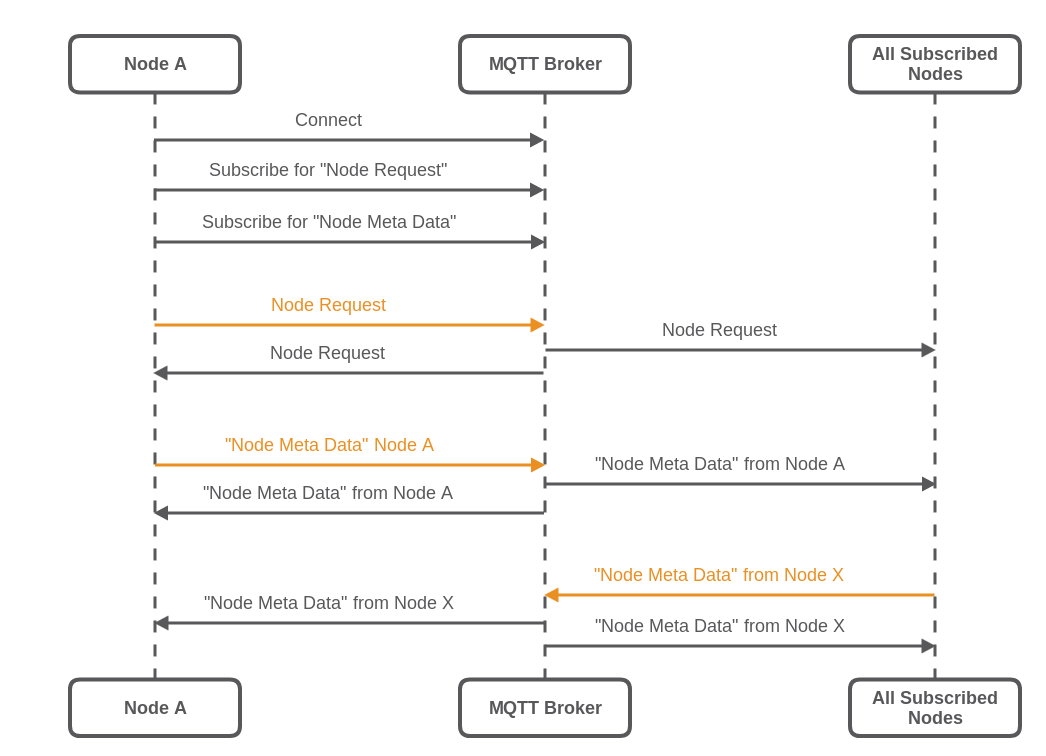
\includegraphics[width=\textwidth]{resources/images/node_discovery.png}
    \caption[Node discovery sequence diagram]{Node discovery sequence diagram}
    \label{fig:node_discovery_squ_dia}
\end{figure}

Figure \ref{fig:node_discovery_squ_dia} shows how the node discovery will be implemented.
Important aspect is that the sender node is also part of the subscribed nodes.
This means after the \textit{connection} to the broker is established and the client is subscribed to the topics, each \textit{Node Request} will also be received by the sender himself.
Benefit out of it, is that beside the fact that a new registered node gets all meta information from all other nodes, also these nodes get the meta information of the new node.
In this way each node has knowledge of all the other nodes and can keep track of them.
That is also the reason why the \textit{"Node Meta Data" from Node A} and \textit{"Node Meta Data" from Node X} are duplicated in figure \ref{fig:node_discovery_squ_dia}.
Beside that the procedure is straight forward: At first one node send out a \textit{Node Request}.
Each subscribed node will get it and send out a response with the \textit{Node Meta Data} to all the other nodes via the broker.
The \textit{after\_connect} handler will be used to send out the \textit{Node Request} after a new nodes is successfully subscribed to the broker.
Before a node disconnects, a \textit{Remove Node} request will be send out, that will inform each node that a specific node will be disappear.
All the nodes react to this by removing the meta data about this node from the database.

\paragraph{ZeroMQServer}
Section \ref{section:ZeroMQ} and \ref{subsection:CommunicationLayer} gave a detailed overview about ZeroMQ and how does it work.
Now the concrete implementation will be discussed.
The wrapper class \textit{ZeroMQServer} binds multiple sockets to the related ports.
There are four sockets binded for the direct node-to-node communication via \ac{TCP} and one port to connect third party applications to the Motey engine.
The latter is used to add or remove capabilities on a node.
ZeroMQ provides an \ac{IPC} protocol for such a use case.
The ZeroMQServer will bind a socket with the Publish-Subscribe pattern that allows multiple publisher to connect to the endpoint.
Two important aspects have to be considered by using the Publish-Subscribe pattern in ZeroMQ.
As in \ac{MQTT} each subscription has to be done to a topic.
Listing \ref{code:ZeroMQ-pub-sub} show the subscription for the \textit{capabilityevent} at line 3.
This also means that it is possible to send multiple different events to a single socket endpoint.
In Motey this feature is not used yet, but nevertheless it is necessary to subscribe to a topic because of the implementation specification of ZeroMQ.
Without that, the subscriber will receive nothing.

\begin{listing}[H]
  \begin{minted}{python}
  def start(self):
    self.capabilities_subscriber.bind('ipc://*:%s' % config['ZEROMQ']['capability_engine'])
    self.capabilities_subscriber.setsockopt_string(zmq.SUBSCRIBE, 'capabilityevent')
    # [...]

  def __run_capabilities_subscriber_thread(self):
    while not self.stopped:
        result = self.capabilities_subscriber.recv_string()
        topic, output = result.split('#', 1)
        self.capability_event_stream.on_next(output)
  \end{minted}
  \caption{Example of the usage of the configreader}
  \label{code:ZeroMQ-pub-sub}
\end{listing}

The second important aspect is at line 9.
An incoming message has always been parsed for a delimiter.
The reason for that is, that the topic, in this case \textit{capabilityevent} have to be prepend to the message followed by the delimiter.
Listing \ref{code:ZeroMQ-capability-event-msg} show such a message.
\begin{listing}[H]
  \begin{minted}{bash}
  capabilityevent#{'capability': 'zigbee', 'capability_type': 'hardware'}
  \end{minted}
  \caption{Example ZeroMQ capability event message}
  \label{code:ZeroMQ-capability-event-msg}
\end{listing}
Therefore the topics and the delimiter has to be removed before the message can be parsed.

The other four sockets are implemented with the Request-Reply pattern and are used to:
\begin{itemize}
  \item reply to a capability request.
  This is used by the \textit{InterNodeOrchestrator} to get the capabilities of other nodes.
  The result is send as a \ac{JSON} string.
  If there are no capabilities an empty \ac{JSON} array will be send.
  \item deploy images is also used by the \textit{InterNodeOrchestrator} to deploy a single image to another node.
  The image model will be transformed to a \ac{JSON} object and send over as a string and vice versa and passed over to the \textit{VALManager} if received.
  \item return the status of an image. This is also used by the \textit{InterNodeOrchestrator} when the state of a service should be fetched. To current state of an image will be detected by the virtualization engine. Afterwards it will transformed to a unified image state. Finally the InterNodeOrchestrator maps the state of all images to the service state.
  \item terminate an existing image instance.
  Only the image id has to be send to perform that action.
  The \textit{VALManager} will handle the termination of the instance.
\end{itemize}
Important aspect while using the Request-Reply pattern, there can only be one connection established at the same time.
In addition a reply must send by the consumer after a request was receive.
As long as there was no message send back, the connection will be blocked and the consumer can not receive any new messages.

As discussed by the other servers, also this one have to be executed in threads.
Difference here is that each socket has its own thread.
This is necessary because each connection waits for a request and has its own request loop.
Therefore each loop would block the main thread.

\paragraph{CommunicationManager}
Finally the \textit{CommunicationManager} is used to decorate the servers from the rest of the source code.
This is helpful for decoupling the components as well as replace or add a new communication component.
Beside that the manager simply forward the methods to the specific server.
It is also used as a central place to start and stop all servers.


\subsection{Capability management}
Similar to the InterNodeOrchestrator the \textit{CapabilityEngine} is used as a connector between the communication layer and the in this case CapabilityRepository.
Therefore the main components of the capability management are the CapabilityEngine and the \textit{ZeroMQServer}.
The latter was extensively described in the previous section and is mainly used to receive new capabilities or to remove them after a request via one of the two ZeroMQ endpoints.
The CapabilityEngine on the other side has two subscriptions to the observer located in the ZeroMQServer.
These subscriptions reacts to add and remove requests of any external application.
Due to the fact that the endpoints are implemented via the ZeroMQ \ac{IPC} protocol only application that are located on the node can interact with the CapabilityEngine.
After a new add service request was received the \ac{JSON} data will be parsed, validated and transformed to the capability model and afterwards stored via the \textit{CapabilityRepository} to the database.
The Removal of an entry is pretty similar.
The received \ac{JSON} data will be again validate with the \textit{capability\_json\_schema} from the schemes model.


\subsection{User interface}
The whole Motey \ac{GUI} is located in a separate folder called \textit{webclient}.
Due to the fact that the \ac{GUI} is only for demonstration purposes, it should not be part of the main engine.
Vue.js the used web framework is pretty lightweight, therefore only two files are necessary to execute the client.
The \textit{index.html} file contains the skeleton of the page.
In addition to that the \textit{main.js} file that is located in the \textit{js} folder contains the business logic of the page.
Figure \ref{fig:motey_gui_screenshot} shows the final \ac{GUI}.
\begin{figure}[H]
    \centering
    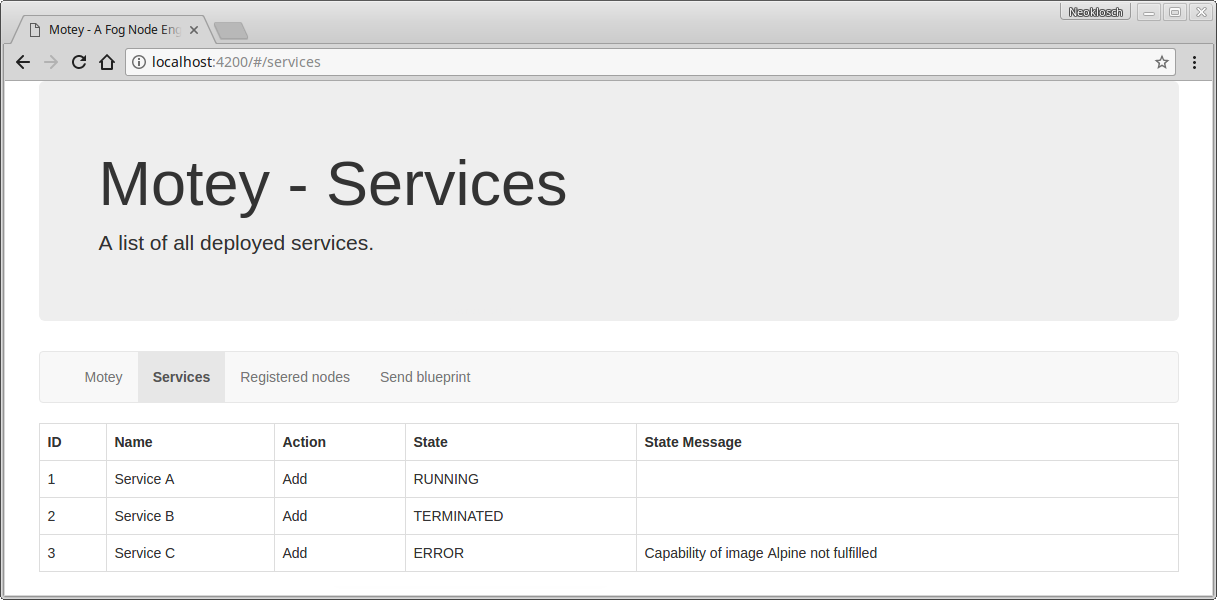
\includegraphics[width=\textwidth]{resources/images/motey_gui_screenshot.png}
    \caption[Screenshot of the Motey \ac{GUI}]{Screenshot of the Motey \ac{GUI}}
    \label{fig:motey_gui_screenshot}
\end{figure}
The header is fixed and only contains the name of the engine and a short description of the page content.
Below them the navigation bar located.
As in the mockup four different pages are available.
The first called \textit{Motey} has a very short introduction into the web client.
The second and also the selected one in the screenshot shows a list with all deployed services.
\textit{Registered nodes} will show a list with all discovered nodes, again in a table.
Finally the \textit{Send blueprint} contains a textarea to put in the \ac{YAML} service description and a button to send the data.

The \textit{index.html} file contains also the files for the bootstrap and Vue.js libraries.
They are loaded from a \ac{CDN} provider to speed up the loading time.
This is possible because if the user already visited a page that uses the same \ac{CDN} provider and the same libraries, they will be cached in the browser internal cache.
If the user then visits another site that try to load the files, they will be taken from the cache instead of requested again.
This increases the page loading speed as well as reduces the traffic.
Another benefit is that the files does not have to be stored on the server.

Beyond that the \textit{main.js} file initializes the routes to handle the navigation bar redirects.
Each route has an own controller similar to the Blueprint concept of the Flask server.
The \textit{NodesListing} and \textit{ServiceListing} controllers mainly fetches the \ac{JSON} data from the \ac{REST} \ac{API} and map them to the related template in the \ac{HTML} file.
The \textit{BlueprintTemplate} controller get the data from the textarea and send them over to the \ac{API}.
Finally the \textit{Content-Type} of the request will be set to \textit{application/x-yaml} as specified in the server endpoint.
As defined before, there is no user authentication or other access control mechanisms due to the fact that this \ac{GUI} is exclusively made for testing purposes.

\subsection{Deployment and Continuous Integration}
Travis CI as the tool of choice for the \ac{CI} uses a \textit{.travis.yml} configuration file.
The content of the file is shown in listing \ref{code:travis_config}.

\begin{listing}[H]
  \begin{minted}{yaml}
  sudo: true
  services: docker
  language: python
  os: linux
  cache: pip
  python:
    - "3.6"

  install: "pip install -r motey-docker-image/requirements.txt"

  script:
    - pycodestyle --ignore=E241,E501 motey/
    - pycodestyle --ignore=E241,E501 samples/
    - python3 -m unittest tests/capabilityengine/test_* tests/communication/test_* tests/models/test_* tests/orchestrator/test_* tests/repositories/test_* tests/utils/test_* tests/val/test_*

  after_success:
    - if [[ "$TRAVIS_BRANCH" = "master" ]]; then
      docker build -t neoklosch/motey motey-docker-image;
      docker login -u="$DOCKER_USERNAME" -p="$DOCKER_PASSWORD";
      docker push neoklosch/motey;
      fi
  \end{minted}
  \caption{Travis CI configuration file}
  \label{code:travis_config}
\end{listing}

There are some important parts in it.
At first the script need root privileges to build and upload Docker images.
Line 1 add this privilege and in line 2 the Docker service is requested.
The programming language the application to build is written in, is declared in line 3, in this case python.
Line 6 and 7 defines the python version to use.
There could be multiple, but due to the fact that the script should only be build one Docker image and should only upload them once, only one python version can be used.
Otherwise multiple python version would be executed and after each successfully build version an container would be build and uploaded.

Line 9 defines the installation script.
This will executed after the virtual environment are created by Travis CI.
In this case the python requirements will be installed.
Line 11 up to 14 are used to test the source code.
A code style check is performed in line 12 and 13.
It will check to code against the \ac{PEP} 8 standard\footnote{\url{https://www.python.org/dev/peps/pep-0008}}, which is be used by several other libraries like the pretty famous Django project\footnote{\url{https://docs.djangoproject.com/en/dev/internals/contributing/writing-code/coding-style}}.
After that all the related unit tests will be executed.
If there is an error during the execution of the \textit{script} block, the whole build process will be stopped and marked as error.
The current state can be view in Travis CI at \url{https://travis-ci.org/Neoklosch/Motey} and also in the readme of the project at \url{https://github.com/Neoklosch/Motey} or \url{http://motey.readthedocs.io/en/latest}.

The \textit{after\_success} block is used to create and upload the Docker image.
Beside that the install routine and also the \ac{CI} commands are similar.
The image will only be executed if it is a master branch build (see line 17).
This is reasonable because a development branch build can be unstable and should not be used to create an official Docker image.
Line 18 will build the image and line 19 uploads it.
Two environment variables are used here, because to upload an image, the username and the password of the Docker Hub account has to be passed.
Due to the fact that this file is under public version control, this sensible information should not be commited.
Therefore preconfigured login credentials are used.
Finally the Docker image will be pushed in line 20.

In the root folder of the Motey project there are two docker image directories.
The first one can be used to create and upload a normal Docker image and it is called \textit{motey-docker-image}.
That folder is also used in the \textit{after\_success} block.
The second folder can be used to build and upload a specific Raspberry Pi Docker image.
Both scripts are slightly different, because a Raspberry Pi is using a \ac{CPU} with an ARM architecture.
Therefore Docker images that should support ARM \acp{CPU} must have specific dependencies and has to be build differently.
To build an image, a so called \textit{Dockerfile} has to be created.
The Dockerfile for the Raspberry Pi image is different to the one for the nomal image, because it load a Raspbian base image instead of an Ubuntu image like the normal file will do.
Also the setup script is slightly different, because Raspbian sometimes need other dependencies or has different preinstalled tools.
Listing \ref{code:motey_dockerfile} shows the Dockerfile for the normal Motey build.

\begin{listing}[H]
  \begin{minted}{dockerfile}
  FROM ubuntu:xenial

  MAINTAINER Neoklosch version: 0.0.1

  ADD ./setup.sh /tmp/setup.sh
  ADD ./requirements.txt /tmp/requirements.txt
  RUN /bin/bash /tmp/setup.sh

  EXPOSE 5023 5091 5092 5094 5094 1883

  CMD ["motey", "start"]
  \end{minted}
  \caption{Dockerfile to create the Motey Docker image}
  \label{code:motey_dockerfile}
\end{listing}

The \textit{FROM} command at line 1 defines the base image.
In this case it is an \textit{Ubuntu} image in version 16.04 also called Xenial Xerus, which has a long-time support and is a pretty stable version.
The \textit{ADD} command is used to add external files to the Docker container to be executed later or make them available in the image.
The script adds a \textit{setup.sh} file that is executed in line 7.
This file uses the \textit{requirements.txt} file, that is also added.
Additional the ports in line 9 are exposed, which means they are provided to the Docker engine as used by the container.
There is no automatic mapping between the host and the guest system ports, but they can be mapped much faster due to the \textit{EXPOSE} command.
Finally the \textit{CMD} command will execute a specific shell command, in this case the \textit{motey start} command.

This command is available after Motey was installed by the \textit{setup.py} file in the root folder.
To install Motey, only two build steps has to be executed, that are shown in listing \ref{code:motey_setup}.

\begin{listing}[H]
  \begin{minted}{bash}
  python3 setup.py build
  python3 setup.py install
  \end{minted}
  \caption{Motey setup procedure}
  \label{code:motey_setup}
\end{listing}

When the installation routine is done, the \textit{motey} command becomes available globally.
The usage of the command line tool was shown in \ref{library:daemonize}.
Beside the installation via the setup script, Motey can also be added as a Docker container named \textit{neoklosch/motey}.
This method is preferred to make the first steps with Motey, because it is more isolated from the host system, easier to use, to remove and to update.

\chapter{Evaluation}
\label{chapter:evaluation}
\minitoc\vspace{.5cm}
In this chapter the implementation of the plugins, based on the previously defined requirements and concepts, are evaluated.
Therefore several performance tests will be analyzed and the code verification will be shown.
Afterwards the final system is demonstrated.

\section{Test Environment}
\label{section:test-environment}
Motey and the performance scripts in section \ref{section:performance-evaluation} was tested on three different devices.
\begin{enumerate}
  \item \textbf{Raspberry Pi 2 Model B Version 1.1} hereinafter called \textbf{NeoPi}, that has a ARM Cortex-A7 \ac{CPU} with four cores each with 900 MHz and a 32-bit architecture. It has 1024 MB \ac{RAM} and a 10/100-MBit-Ethernet port. The device is running a Raspbian 8 (jessie) with Linux Kernel version 4.9.
  \item \textbf{Raspberry Pi 3 Model B Version 1.2} hereinafter called \textbf{BuffPi}, is the currently the newest Raspberry Pi on the market. It has a ARM Cortex-A53 \ac{CPU} also with four cores, but each has 1200 MHz and 64-bit architecture. It also has 1024 MB \ac{RAM} and a 10/100-MBit-Ethernet port.  This devices is also running Raspbian 8 (jessie) with Linux Kernel version 4.9.
  \item \textbf{Acer Aspire V5-573G} hereinafter called \textbf{Laptop}, with an Intel Core i7-4500U \ac{CPU} with two cores each 1.80 GHz and a 64-bit architecture as well. It has 8 GB \ac{RAM} and a 802.11n WiFi connection. It is running a Linux Mint 18.1  64-bit \ac{OS} with a Linux Kernel version 4.4.
\end{enumerate}

Both the \textit{NeoPi} and the \textit{BuffPi} are connected via ethernet to a router.
The \textit{Laptop} is connect via 802.11n WiFi to the router.
% TODO: network information, multiple devices, etc.

\section{Performance Evaluation}
\label{section:performance-evaluation}
In the following section some performance relevant tests are shown and analyzed.
Especially the performance of the used virtualization method is crucial for the system as well as the connection performance of the used protocols are important.
All evaluations are made with low power devices in mind.
This means a small overhead and a fast and lightweight solution is preferred.

\subsection{Docker vs. Hypervisor-Based Virtualization}
Due to the fact that Docker is the core component in the created prototype, it is important to verify the performance on low power devices.
Unfortunately a performance comparison with established \ac{VM} tools like VMWare or Xen on a Raspberry Pi is not possible, because nearly all of them does not support the ARM \ac{CPU} architecture.
There are several performance tests on x86 architecture.
IBM for example compared \acp{VM} or more specific \acp{KVM} with Docker in a research report\autocite{IBM:Performance:2014} from 2014.
They conclusion was that \ac{KVM} has a significant overhead to every I/O operation.
Therefore it is less suitable for latency-sensitive workloads or high I/O rates.
Figure \ref{fig:ibm_kvm_docker_io} show the throughput for random I/O operations for a native, a Docker virtualized and a \ac{KVM} virtualized system.

\begin{figure}[H]
    \centering
    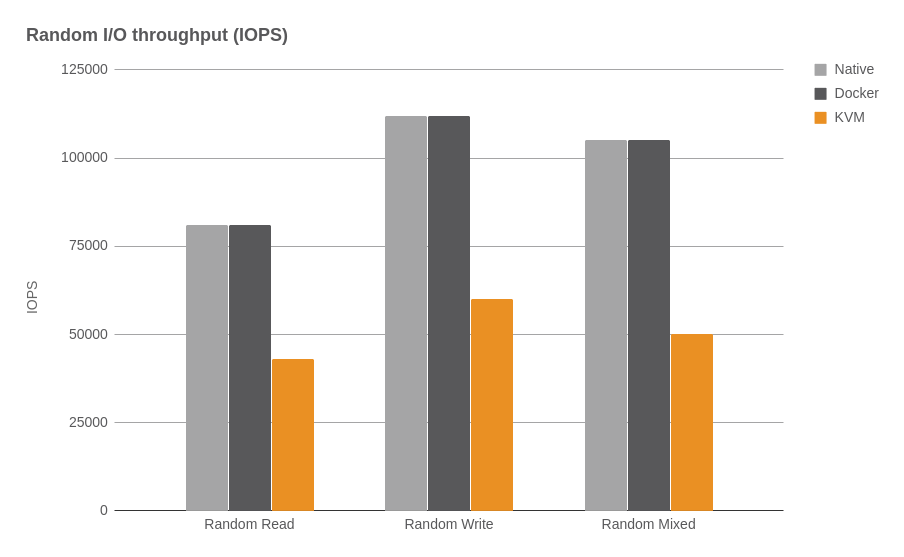
\includegraphics[width=\textwidth]{resources/images/performance_ibm_kvm_docker_io.png}
    \caption[KVM and Docker I/O throughput comparison by IBM]{KVM and Docker I/O throughput comparison by IBM. Adapted from: \autocite[p. 6]{IBM:Performance:2014}}
    \label{fig:ibm_kvm_docker_io}
\end{figure}

Compared to the native system, Docker has "nearly no overhead"\autocite[p. 6]{IBM:Performance:2014}.
But also Docker has some drawbacks.
For example it has an overhead for workloads with high packet rates.\autocite[cf.][p. 6]{IBM:Performance:2014}
The overall conclusion by IBM was that Docker is more performant than a \ac{KVM} virtualized system.
\newpage
Another benchmarking comparison\autocite{Russell:Performance:2014} between Docker and \ac{KVM} that was also made by IBM show a much clearer result.
In this test Docker is much more performant in nearly every point of view.
It has less overhead in terms of \ac{CPU} usage\autocite[cf.][p. 25]{Russell:Performance:2014}, memory performance\autocite[cf.][p. 50]{Russell:Performance:2014} and boot time\autocite[cf.][p. 24]{Russell:Performance:2014}.
Only the network throughput is nearly the same.\autocite[cf.][p. 52]{Russell:Performance:2014}
Concluding also the container size is much smaller in Docker than in \ac{KVM}.\autocite[cf.][p. 66]{Russell:Performance:2014}\newline

\autocite{Ramalho:2016} consolidates this statement of IBM.
Docker is nearly no performance loss compared to the Hypervisor-based virtualization, in this case \ac{KVM}.\autocite[cff.][p. 3]{Ramalho:2016}
The only are where Docker can not keep up with a native environment, is while performing network request and response.
In direct comparison, Docker only can perform around half of the transactions as a native environemnt is able to do.\autocite[cf.][p. 6]{Ramalho:2016}
Compared to \ac{KVM} Docker has a significant performance advantage.
In all of the tested areas "the hypervisor-based solution showed a significant overhead that cannot be easily mitigated"\autocite[p. 6]{Ramalho:2016}.
Overall Docker is much more lightweight and due to the fact that it supports the ARM architecture, it is well suitable for the usage on low power devices.

\subsection{Performance HTTP}
To test the \ac{HTTP} performance of the application two simplified test scripts are created.
Both are located in the \textit{performance\_tests/http} folder in the Motey project.
The \textit{server.py} script starts a Flask server and waits for a POST request.
If it gets one it will send back a static container id.
The \textit{client.py} script is used to send the \ac{JSON} data to the server.
It is an extract of an Docker image command as it would be used in the Motey application.
Afterwards 10.000 request will be send to the server.
This execution is one iteration of the test.
In total 10 iterations are performed to get an result.
An overview of all test results are shown in section \ref{appendix:http_test_results}.
Figure \ref{fig:performance_http_server_comparison} shows the result of the tests.

\begin{figure}[H]
    \centering
    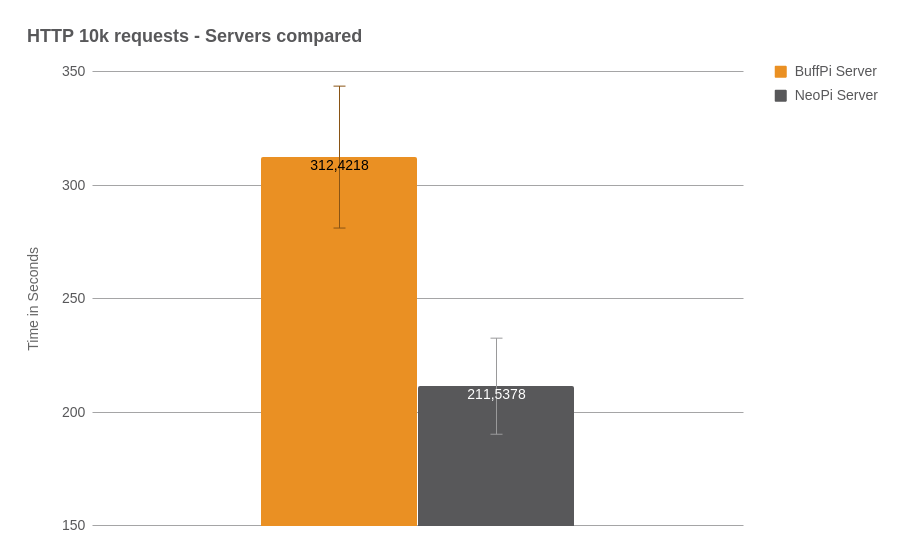
\includegraphics[width=\textwidth]{resources/images/performance_http_server_comparison.png}
    \caption[HTTP 10k requests - Server comparison]{HTTP 10k requests - Server comparison}
    \label{fig:performance_http_server_comparison}
\end{figure}

There are two bars indicating the time needed to send 10.000 requests: the left one, that represents a setup where the more powerful BuffPi was the server and the NeoPi was the client, tokes in total more time, then the setup where the NeoPi is the server.
This is a surprising outcome because the assumption was that the server tokes more computation time then the client.
But the results prove the opposite.
If the less powerful device is the server the packages are much faster sent the vice versa.
Overall using \ac{HTTP} as the protocol of choice, the messaging is pretty slow.
To send the 10.000 request even the faster setup toke 03:31 minutes.
This result depends on the huge package overhead in \ac{HTTP} and also the need for waiting for the request.
Such a setup is fits well for simple status or rarely sent deployment requests, but not for high frequently used inter-node connections or in a low latency environment.

\subsection{Performance ZeroMQ}
Also for the ZeroMQ performance test both Raspberry Pis are used to communicate with each other.
Similar to the \ac{HTTP} test the BuffPi and the NeoPi are switch between server and client.
To test the ZeroMQ performance, the test has to be splitted up into two different variants.
The first one is called \textit{\ac{CC}}.
This means, once a ZeroMQ connection is established, all of the 10.000 request are send via this one session.
\textit{\ac{NC}} is used to simulate the case where each connection has to be closed before a new request will be send.
This is more realistic to the implementation in Motey, because the connection to one node will established in the moment they are needed and closed as soon as the request is done.\newline

Beside that the test setup is the same like in the \ac{HTTP} performance test.
The scripts are located in \textit{performance\_tests/zeromq} folder, the \textit{server.py} script is the same for both variant, only the client scripts differ.
Each client send out 10.000 requests and each iteration is performed ten times.
The total test results are in section \ref{appendix:zeromq_test_results}.

\begin{figure}[H]
    \centering
    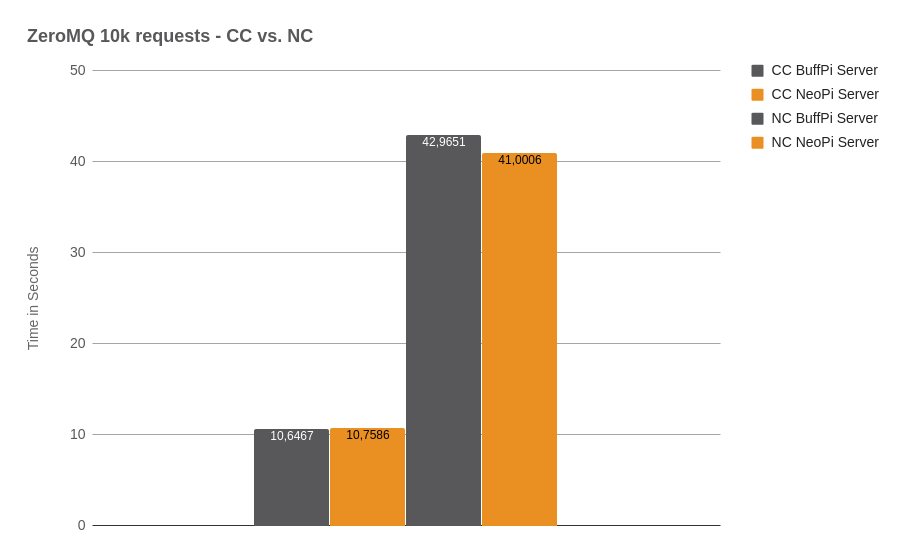
\includegraphics[width=\textwidth]{resources/images/performance_zeromq_cc_vs_nc.png}
    \caption[ZeroMQ comparison between new connection and constant connections]{ZeroMQ comparison between new connection and constant connections}
    \label{fig:performance_zeromq_cc_vs_nc}
\end{figure}

The difference between the \ac{CC} and \ac{NC} is significant.
The \ac{CC} is around four times faster then the \ac{NC}.
Certainly this relates to the connection and disconnection phase of the socket.
On the other side the difference between the two devices is minimal and can be neglected in this evaluation.
The comparison between ZeroMQ and \ac{HTTP} is much more crucial.
Compared to the \ac{CC} \ac{HTTP} is around 20 times slower.
Even compared to the \ac{NC} it is around 5 times slower.
Figure \ref{fig:performance_zeromq_vs_http} shows the test results.

\begin{figure}[H]
    \centering
    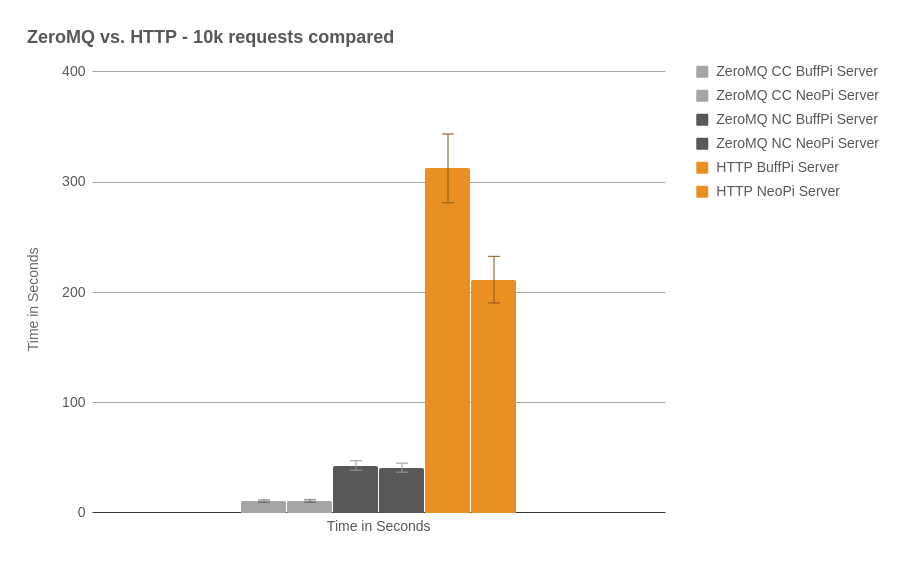
\includegraphics[width=\textwidth]{resources/images/performance_zeromq_vs_http.png}
    \caption[Performance comparison ZeroMQ vs. HTTP]{Performance comparison ZeroMQ vs. HTTP}
    \label{fig:performance_zeromq_vs_http}
\end{figure}

In addition to that \ac{HTTP} have a huge packet overhead that will consume more network bandwidth.
ZeroMQ is well suitable for low latency connections and on the same side more lightweight.
In the test ZeroMQ is always used in \ac{TCP} mode.
The creator of ZeroMQ promise that the \ac{IPC} and especially the inter-thread protocol are much faster than \ac{TCP}.\autocite[cf.]{ZeroMQ:UicastTransports}
But still for the \ac{TCP} mode, the results are self-evidently.


\subsection{Performance MQTT}
The last test setup was used to test the MQTT performance.
Due to the fact that MQTT need a broker to be executed a third device the \textit{Laptop} was added.
Each test was setup in three different ways.
The Laptop, the BuffPi and the NeoPi were the broker each at a time.
The BuffPi or the NeoPi were always the publisher and the receiver.
Furthermore MQTT has three different types to be executed, which is called the \ac{QoS} level.
The \ac{QoS} was explained in section \ref{section:MQTT}.
The initial assumption was that each level has a different performance.
Also in this setup each request was sent 10.000 times and in ten iterations.
All results are shown in section \ref{appendix:mqtt_test_results}.
Figure \ref{fig:performance_mqtt_average_time_all_qos} shows the average time for each \ac{QoS} level where BuffPi was the broker as well as the publisher and the NeoPi was the consumer.

\begin{figure}[H]
    \centering
    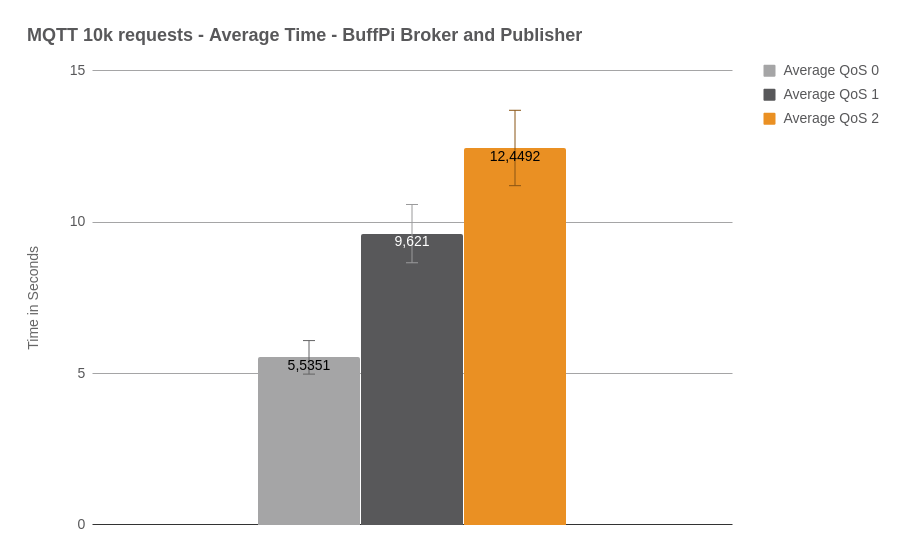
\includegraphics[width=\textwidth]{resources/images/performance_mqtt_average_time.png}
    \caption[MQTT average time for all QoS levels]{MQTT average time for all QoS levels}
    \label{fig:performance_mqtt_average_time_all_qos}
\end{figure}

As expected the \ac{QoS} level performance differ significantly.
The difference between \ac{QoS} 0 and \ac{QoS} 2 is more than two and a half of the time used for sending out the 10.000 requests.
Therefore the \ac{QoS} level should be consciously used in the required use case.
Due to the fact that the MQTT system is used for the node discovery a lower \ac{QoS} level is suitable.
\ac{QoS} level 1 is recommended for that application.
And even compared to the \ac{HTTP} connection, MQTT is much faster and more reliable for the node discovery.\newline

On the other side, the device that is executing the broker is much more crucial.
Figure \ref{fig:performance_mqtt_average_time_qos_1} shows the difference between the three devices.\newline

The Laptop that has the most powerful hardware is also much faster by sending out the messages.
NeoPi the weakest device in the test setup tokes nearly as twice as the Laptop.
Compared to \ac{HTTP} even the NeoPi is much faster, but for a huge cluster the broker should be as powerful as possible.
If possible the broker should be located in the cloud.
There it has the better hardware and can also be better maintained.
Nevertheless also a node in the fog node cluster can be used to act as a broker.
It would be optimal to use a dedicated node for that job.

\begin{figure}[H]
    \centering
    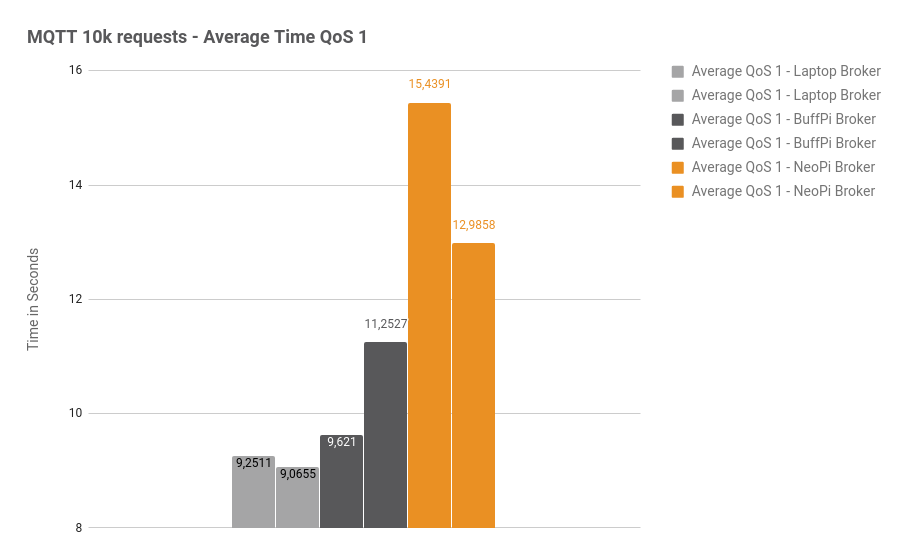
\includegraphics[width=\textwidth]{resources/images/performance_mqtt_average_time_qos_1.png}
    \caption[MQTT average time for QoS 1]{MQTT average time for QoS 1}
    \label{fig:performance_mqtt_average_time_qos_1}
\end{figure}

One important learning about MQTT, in \ac{QoS} level 1 and 2 messages has to be persisted in a local cache.
This took some time and it is possible that if the receive message on the broker exceed the message queue.
If this happens all following messages from that node will be dropped.
To fix that issue the total amount of messages in the queue must be extended.
Therefore the Mosquitto config has to be configured by adding the following lines:

\begin{listing}[H]
  \begin{minted}{bash}
  max_inflight_messages 1000
  max_queued_messages 10000
  \end{minted}
  \caption[Mosquitto config modification to fix the messages dropped issue]{Mosquitto config modification to fix the messages dropped issue}
  \label{code:performance_mosquitto_config}
\end{listing}

The first parameter adjust the maximum number of "messages that can be in the process of being transmitted simultaneously"\autocite{Mosquitto:Conf:Documentation}.
The \textit{max\_queued\_messages} modify the maximum number of messages that can be hold in the queue.\autocite[cf.]{Mosquitto:Conf:Documentation}
Especially this number has to be increased in the tests, because the scripts sends out a huge amount of publish calls in a very short time.
In general these numbers has to be adjusted specifically for each use case.
Furthermore these configs are only important if a \ac{QoS} level 1 or 2 is used, because level 0 does not persist any messages.

\chapter{Conclusion}
\label{chapter:conclusion}
\minitoc\vspace{.5cm}
This final chapter sums up the thesis as well as the created prototype called Motey.
The first section outlines the initial idea behind the project and reproduce the different work stages.
Issues that remained unsolved are described in the last section as well as an outlook for the Motey project is shown.

\section{Summary}
Objective of this thesis was the "Design and Development of a Fog Service Orchestration Engine for Smart Factories".
Therefore a prototype for such an orchestration engine called Motey was created.
The application was created in cooperation with the \acf{FOKUS}.
The main idea of the project was worked out in an iterative process together with supervisors of the \ac{FOKUS}.
In several meetings the objectives was analyzed and elaborated.
Motey is designed to be executed on each fog node and is able to instantiate an inter-node connection.
Each node has knowledge of all the other nodes and can communicate with them right at the moment they have to.\newline

The application is also able to handle different so called capabilities.
That are functional and non-functional requirements a node can fulfill.
These capabilities are used to deploy images, for example \acp{NF} to a one or more nodes.
The node that receives a deployment schema check the requirements of the contained images and deploy them on the same node if it is possible or on other nodes that are able to deploy them.
Labels can be configured from within the node itself or from any external application.
Finally an image will be started via the related virtualization tool.
In case of the prototype and as a primary requirement of this project, Docker is the default engine.
For the inter-node communication the ZeroMQ and \ac{MQTT} protocols are used.
They are much faster than the pretty famous \ac{HTTP} protocol, as shown in the performance evaluation section \ref{section:performance-evaluation}.
An \ac{HTTP} \ac{REST} \ac{API} is also available to enable compatibility with well known cloud orchestration engines like Open Baton or OpenStack.

The whole application is well documented and tested.
Each component has a related unit test and the documentation is available online at \url{https://neoklosch.github.io/Motey/}.
A \ac{CI} pipeline is used to automatically build each new version, test them and finally deploy them as a Docker image to the Docker Hub.
This is especially useful to reduce the overhead of repeating tasks, to guarantee the correctness of the current version and also to have an up-to-date version available via the Docker infrastructure.

Biggest challenges in this project were to create a fast and lightweight inter-connection between the nodes, that was achieved by the protocols of choice ZeroMQ and \ac{MQTT}, as well as the abstraction of the virtualization underlying virtualization tools.
The latter partly kept unsolved, because only a few virtualization tools supports the ARM \ac{CPU} architecture.
Whereas ARM is a common architecture on low power devices.
Therefore the integration of famous virtualization tools is not possible at the moment.
Due to the fact that \ac{IoT} becomes more and more important in the next years hopefully also the tools will adjusted in this direction.
However Docker as the main virtualization tool in this thesis is available for ARM \acp{CPU} yet and also implemented in Motey.
As a lightweight solution for virtualization this is a good starting point so far.

% \section{Dissemination}
% Who uses your component or who will use it? Industry projects, EU projects, open
% source...? Is it integrated into a larger environment? Did you publish any papers?

% integration in open baton denkbar
% als weiterentwicklung für arbeiten im bereich autonomous deployment in fog
% Smart Factories
% Papers planed (?)
%
% Currently Motey is released as an Open Source project at Github \url{https://github.com/Neoklosch/Motey}.
% The basic idea is to use this as a solid fundermental for bigger projects inside the \ac{FOKUS}.
%
% \doit

% \section{Impact}
% \label{section:summary_impact}
% Summarize the main problems. How did you solve them? Why didn’t you solve them?


% node discovery
% -> central broker where each node have to registered to
% -> information on each new node

% virt on low power devices
% -> docker
% -> XEN & Co not possible

% capabilities
% -> external API
% ---> ZeroMQ

% Inter node connection
% -> node discovery + ZeroMQ

% didn't solved -> real autonomous behavior
% didn't solved -> access managemnt and so on
% \doit

\section{Outlook}
Motey is a well developed and pretty solid basis for further development.
As in every bigger project, Motey has significant room for improvements.
For example the autonomous behavior can be improved a lot.
One possibility could be to implement much more responsibility in case of the absence of the centralized fog level.
One of the nodes could become a master node.
These nodes then can act as a delegate for the centralized level.
It can be track the state of the other nodes and can react to unexpected issues.
Another possibility could be an improved access control or right management.
Some nodes could have more rights than others.
Therefore an hierarchy could be created and sensitive images or images that handle sensitive data could be easily identified.
Especially for security reasons that becomes very important.\newline

The node discovery can be improved by making the \ac{MQTT} broker replaceable.
This could be achieved by having an logic that moves the broker over to a node that is up and running if the broker disappears.
Such a behavior makes the system reliable and again more autonomously.
Finally the integration of third party applications can be ensured.
For example the integration of Open Baton as the centralized orchestrator could be realized.
Also node specific tools like a hardware detection engine, that can deploy images or at least add new capabilities to Motey based on the connected hardware are imaginable.\newline

Motey can be seen as a good starting point for a complex environment made for fog computing.
It is easy to extend, is lightweight during execution and networking.
Due to the fact that it can be deployed via Docker out of the box it is easy to test and the documentation and the unit test should help to understand the fundamentals pretty easy.
At the end the created project successfully reveal that the developed concept works out pretty well in a prototypical quality.
The result can thus be considered as solid basis for further development.


\nolinenumbers
\cleardoublepage

\appendix
\pagenumbering{Roman}
\setcounter{page}{1}
\cleardoublepage
\chapter{A Test Results}
\minitoc\vspace{.5cm}

\section{Performance Test Results}\index{Performance Test Results}

\subsection{HTTP}\index{HTTP}
\label{appendix:http_test_results}
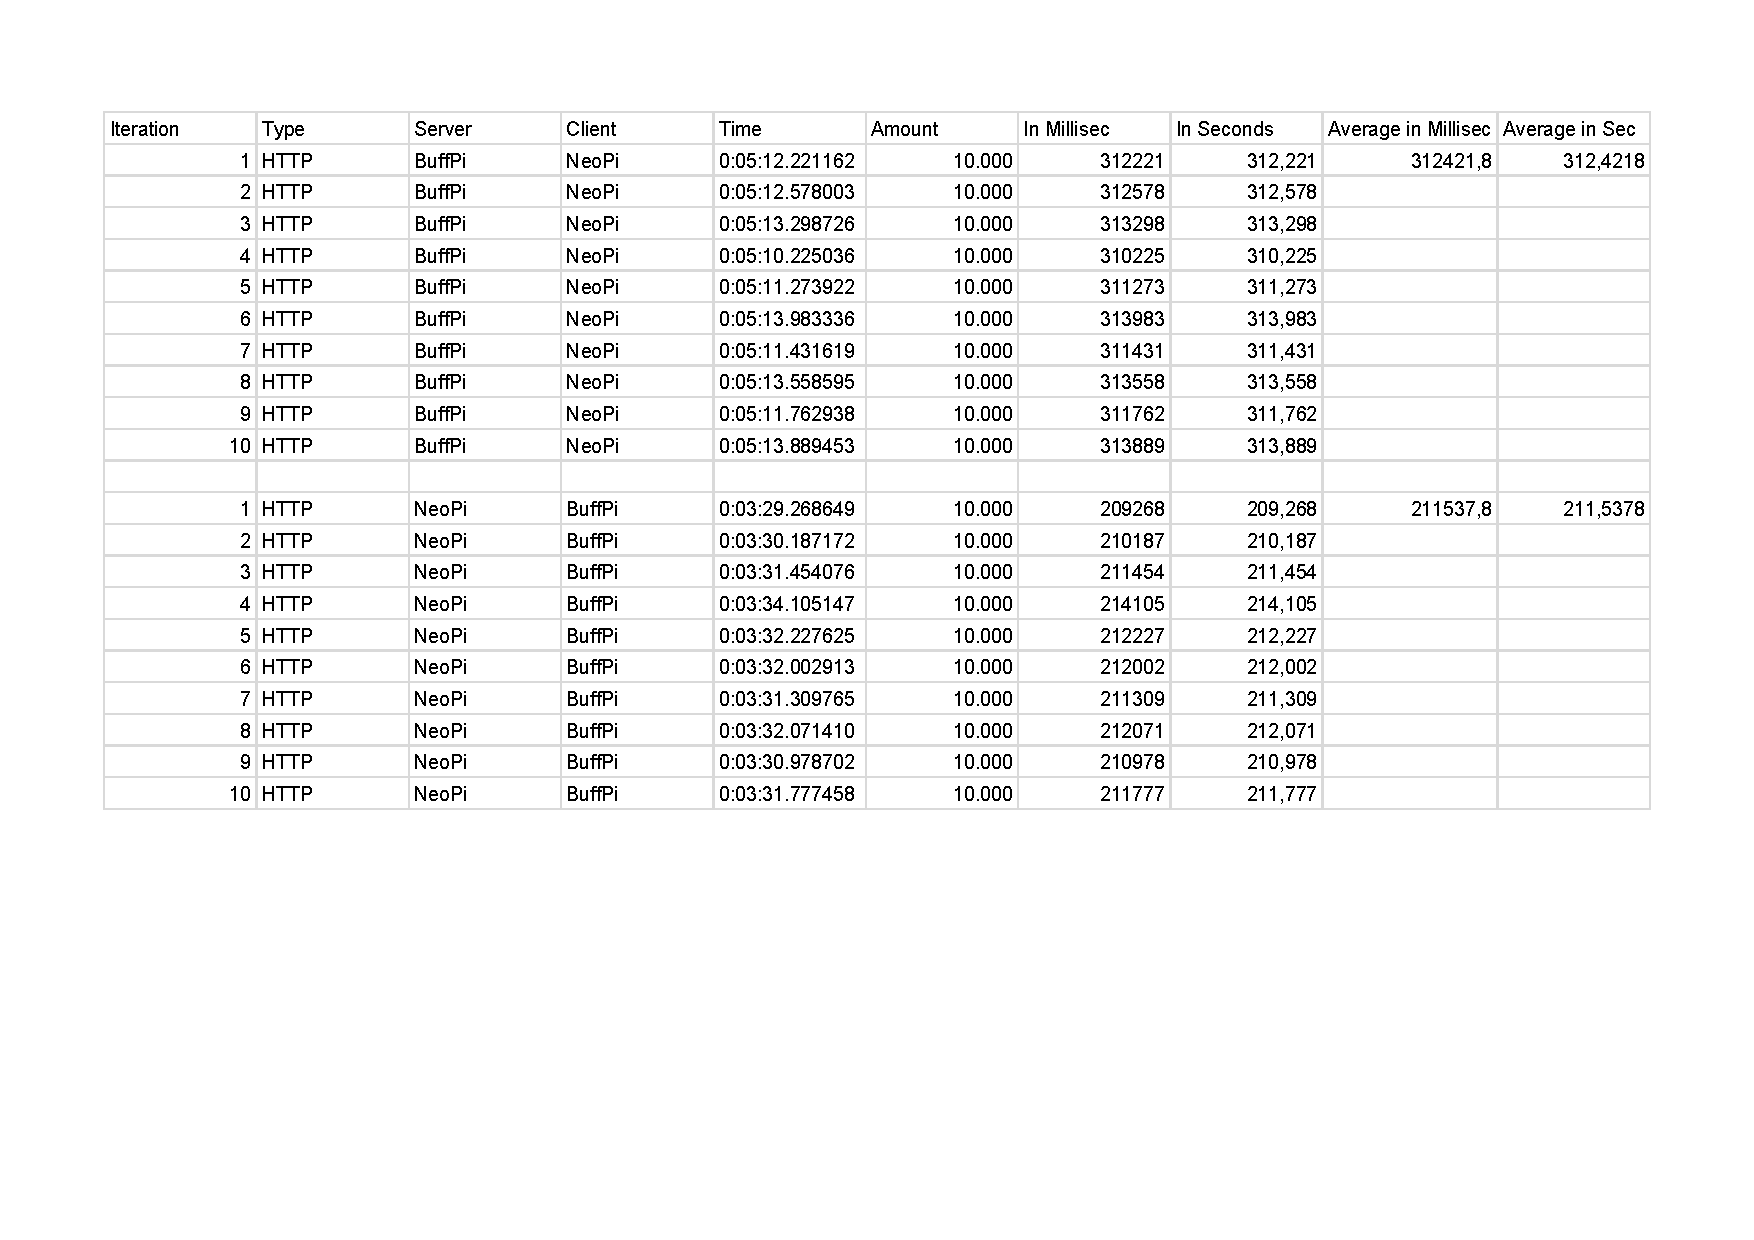
\includepdf[pages=-,landscape]{resources/pdfs/MA_Testergebnisse_-_HTTP.pdf}

\subsection{MQTT}\index{MQTT}
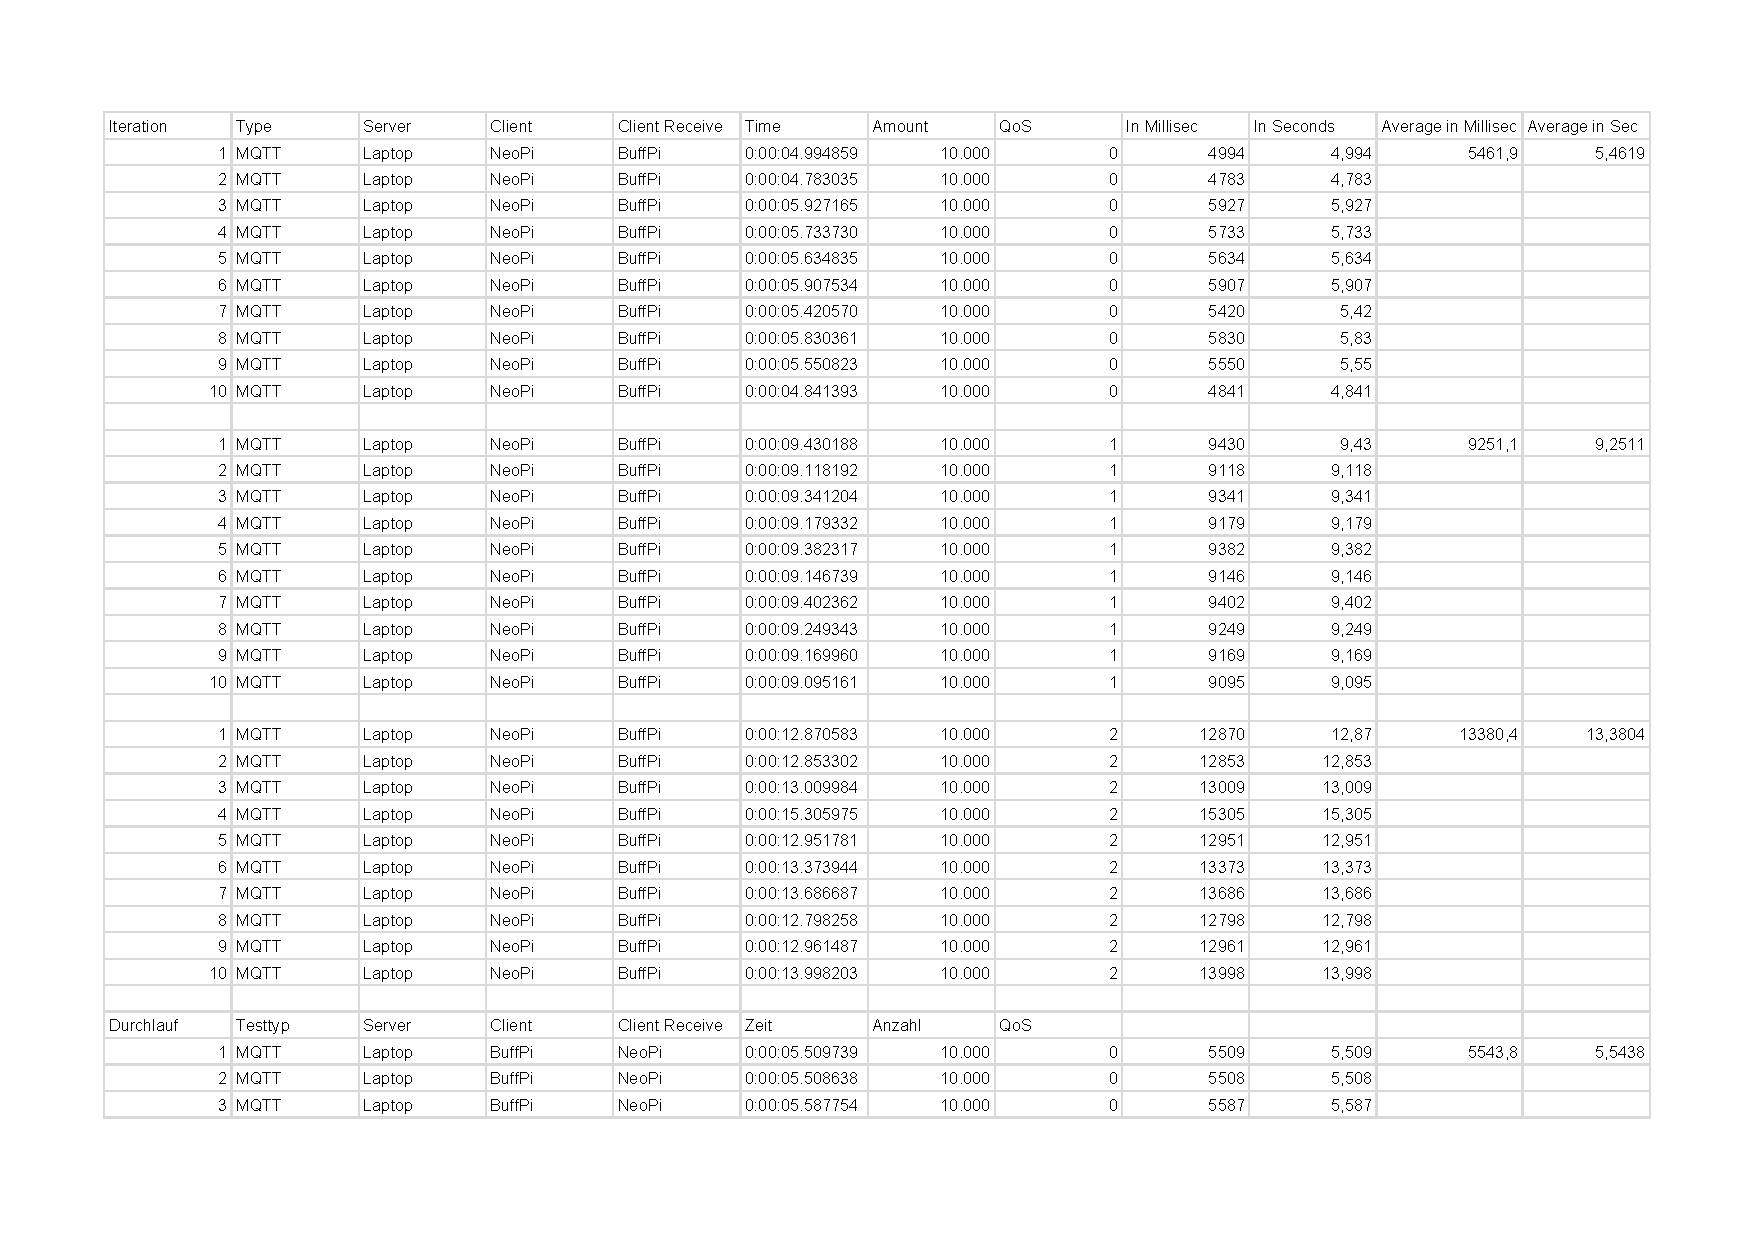
\includepdf[pages=-,landscape]{resources/pdfs/MA_Testergebnisse_-_MQTT.pdf}

\subsection{ZeroMQ}\index{ZeroMQ}
\label{appendix:zeromq_test_results}
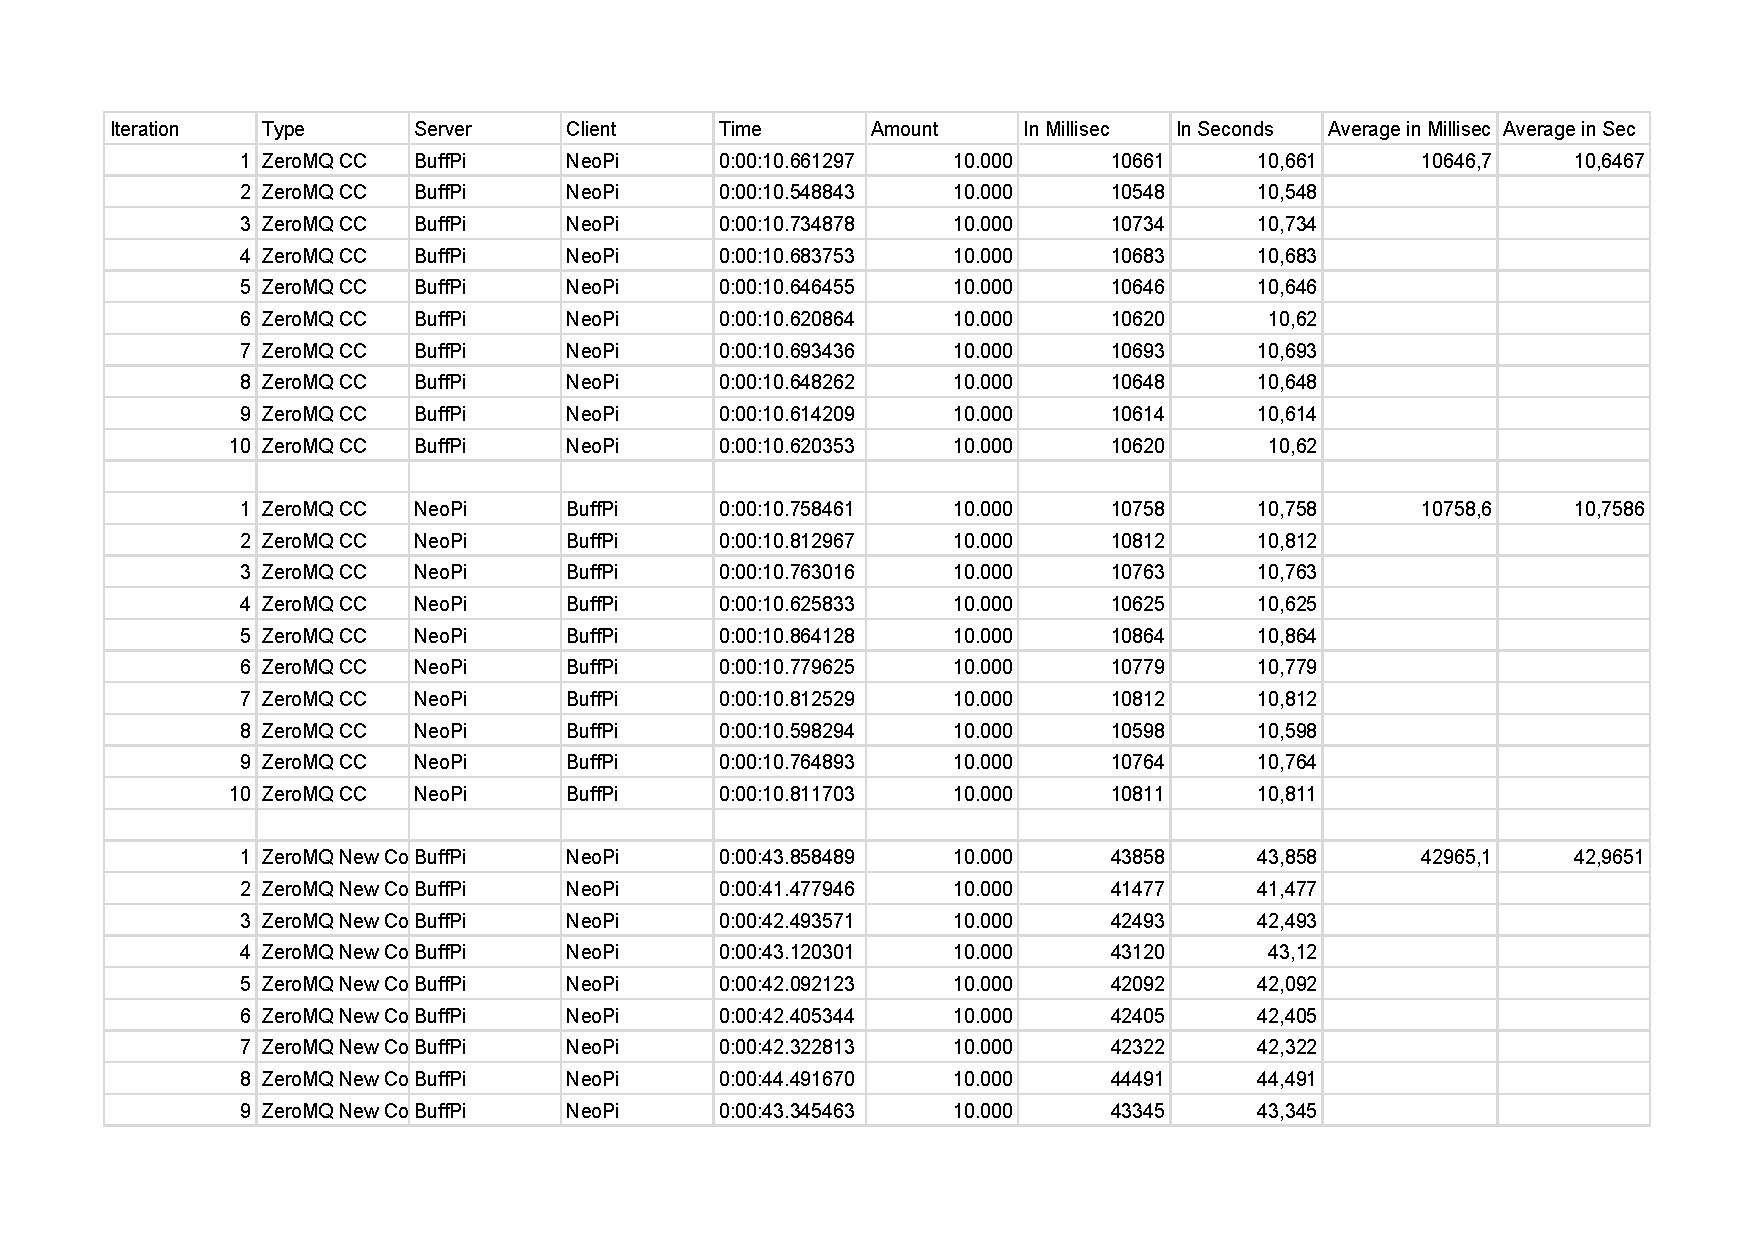
\includepdf[pages=-,landscape]{resources/pdfs/MA_Testergebnisse_-_ZeroMQ.pdf}

\section{Performance Test Graphs}\index{Performance Test Graphs}

\subsection{HTTP Graphs}\index{HTTP Graphs}
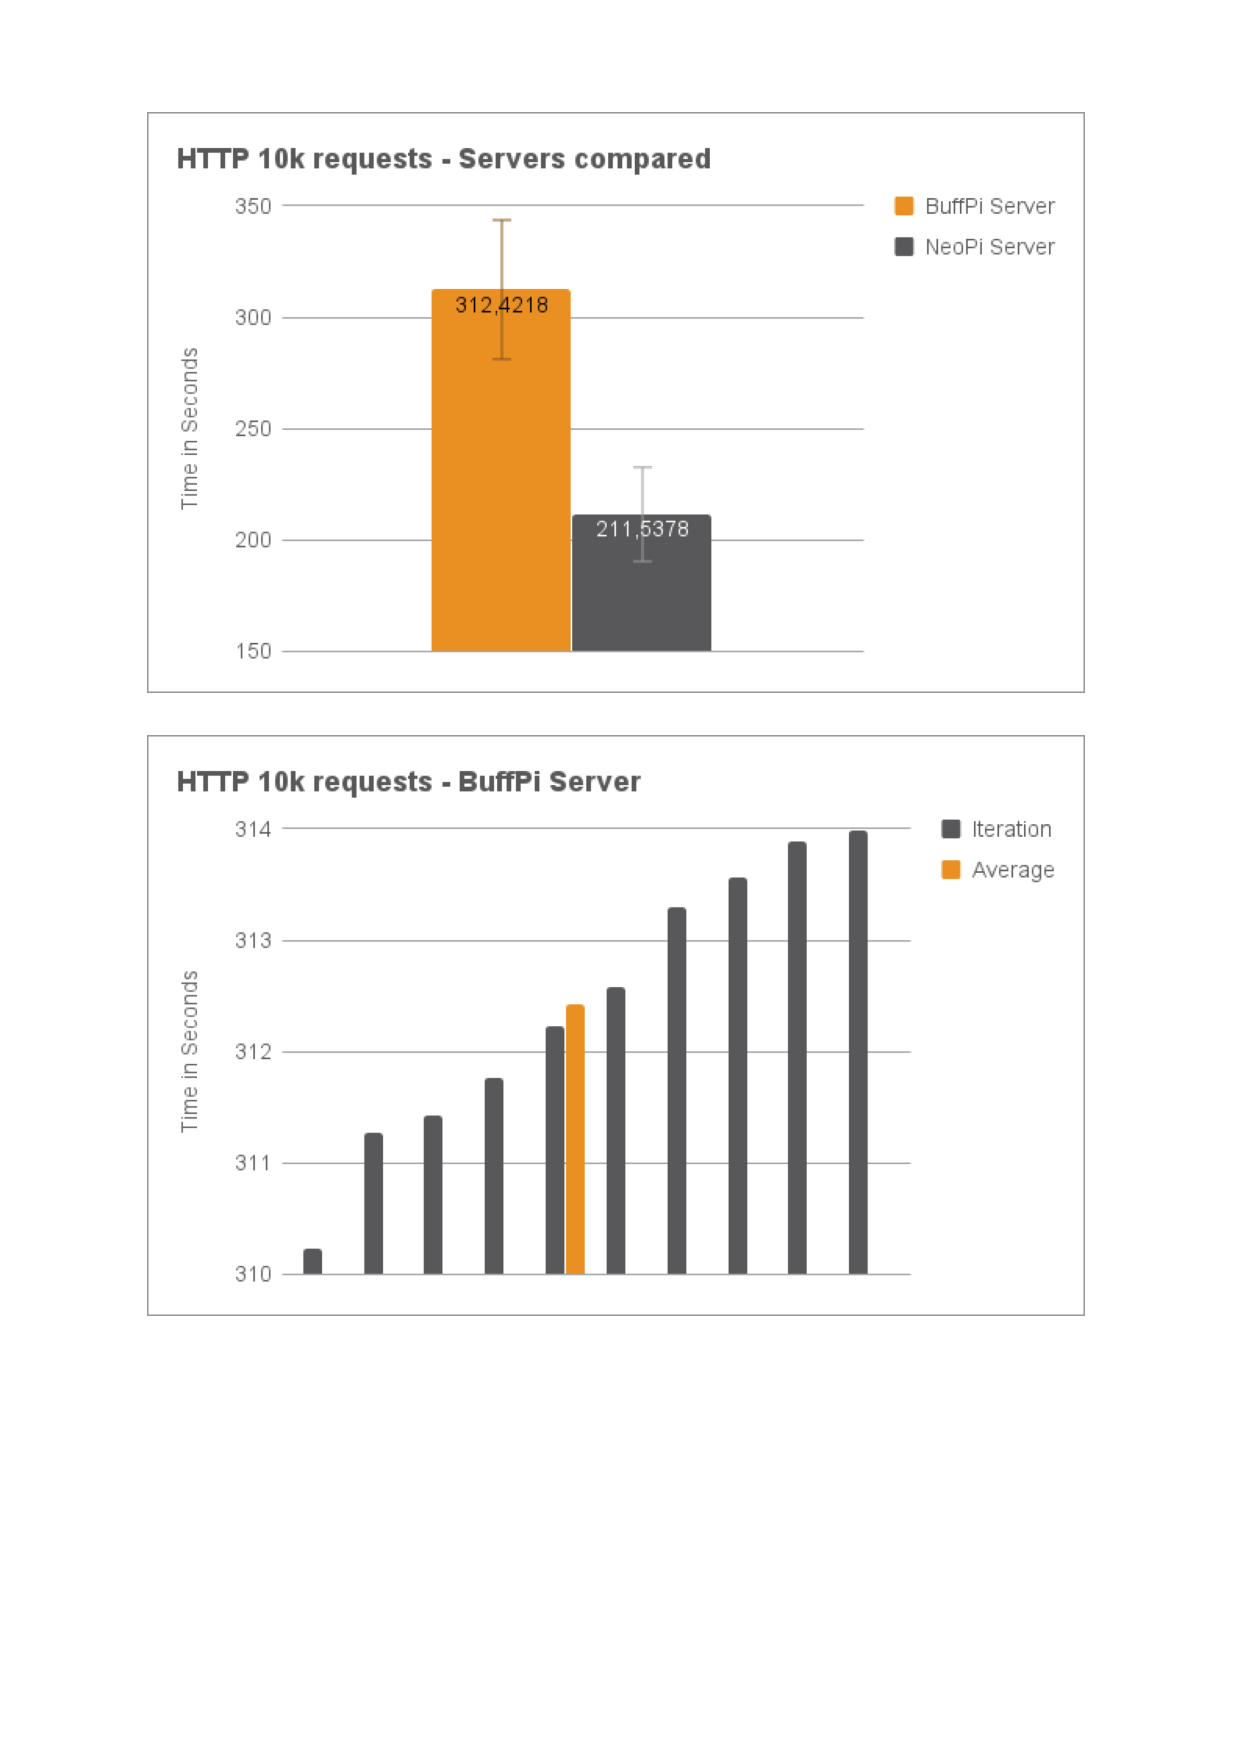
\includepdf[pages=-]{resources/pdfs/MA_Testergebnisse_-_HTTP_Graphs.pdf}

\subsection{MQTT Graphs}\index{MQTT Graphs}
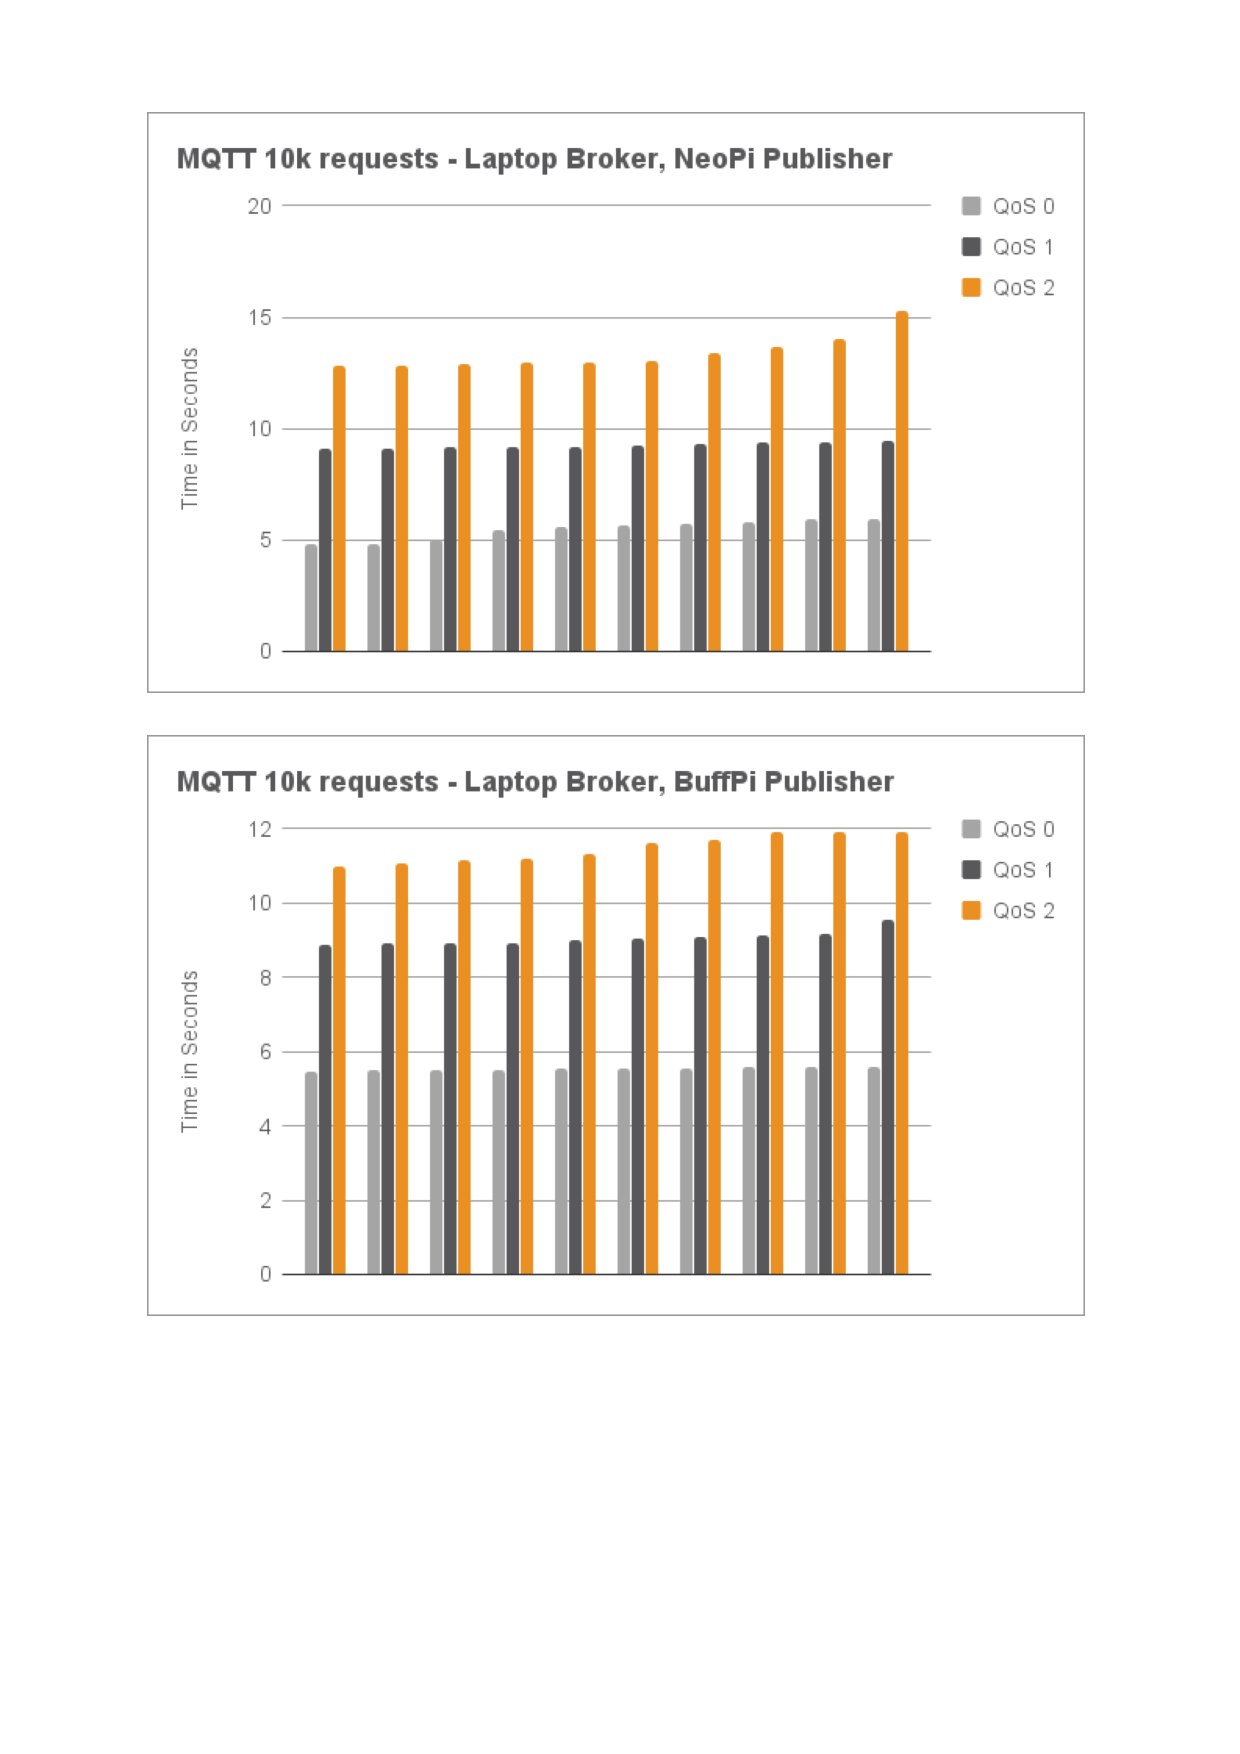
\includepdf[pages=-]{resources/pdfs/MA_Testergebnisse_-_MQTT_Graphs.pdf}
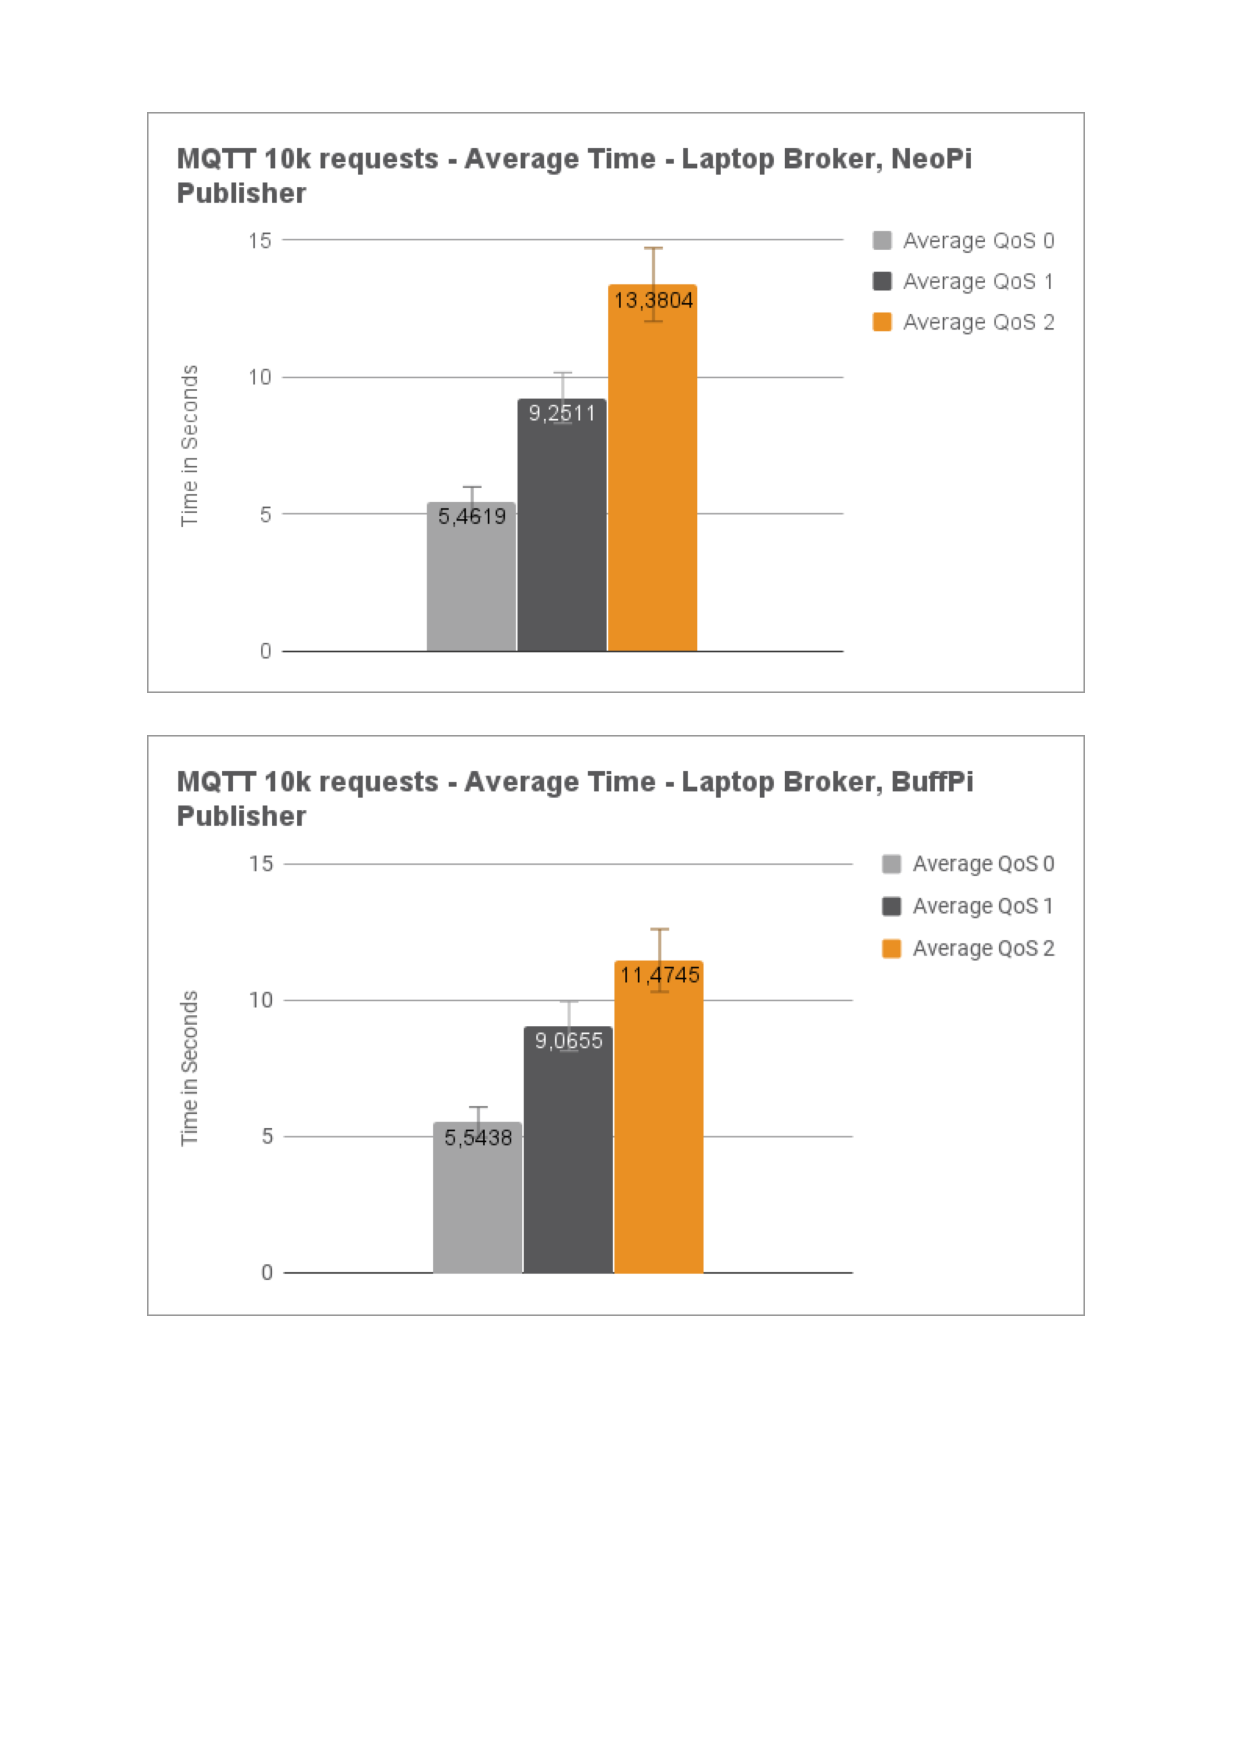
\includepdf[pages=-]{resources/pdfs/MA_Testergebnisse_-_MQTT_Graphs_Average.pdf}
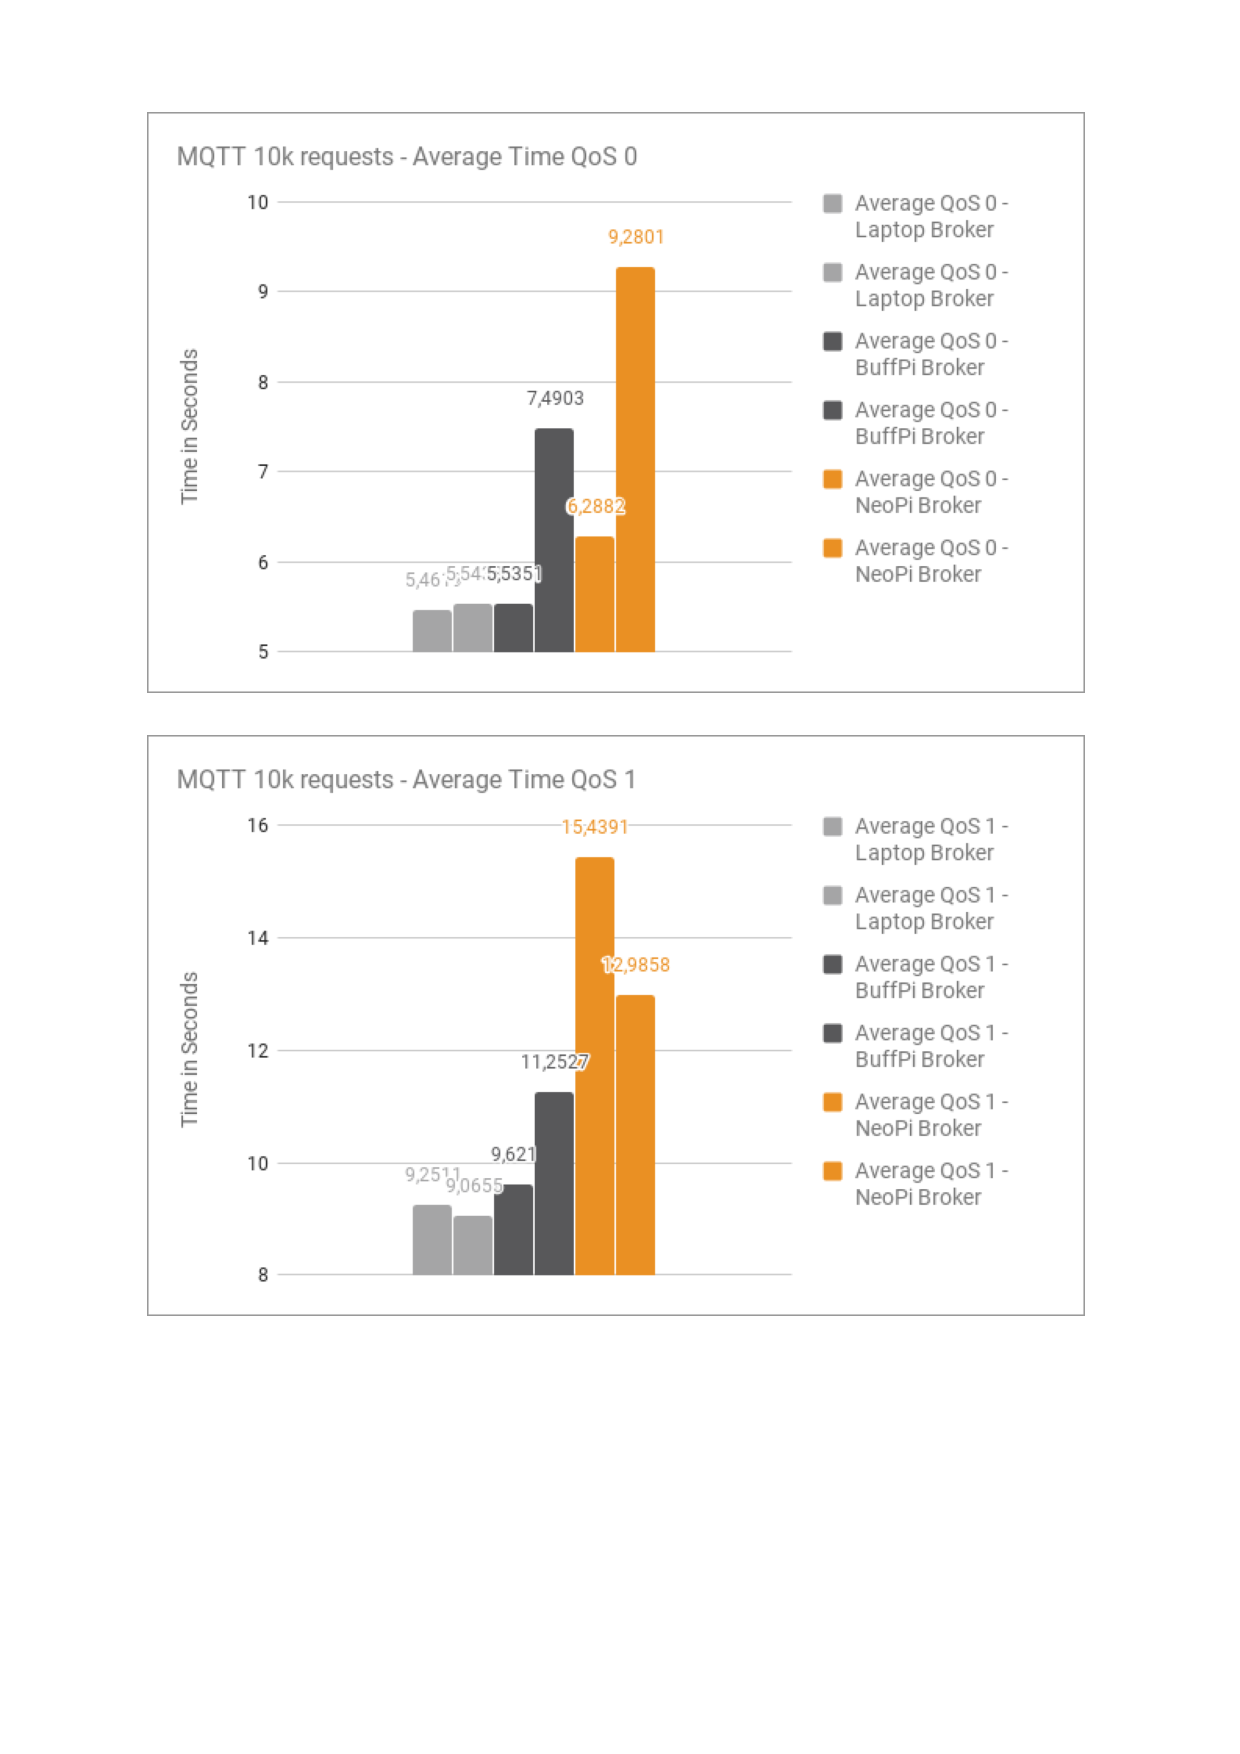
\includepdf[pages=-]{resources/pdfs/MA_Testergebnisse_-_MQTT_Graphs_QoS.pdf}

\subsection{ZeroMQ Graphs}\index{ZeroMQ Graphs}
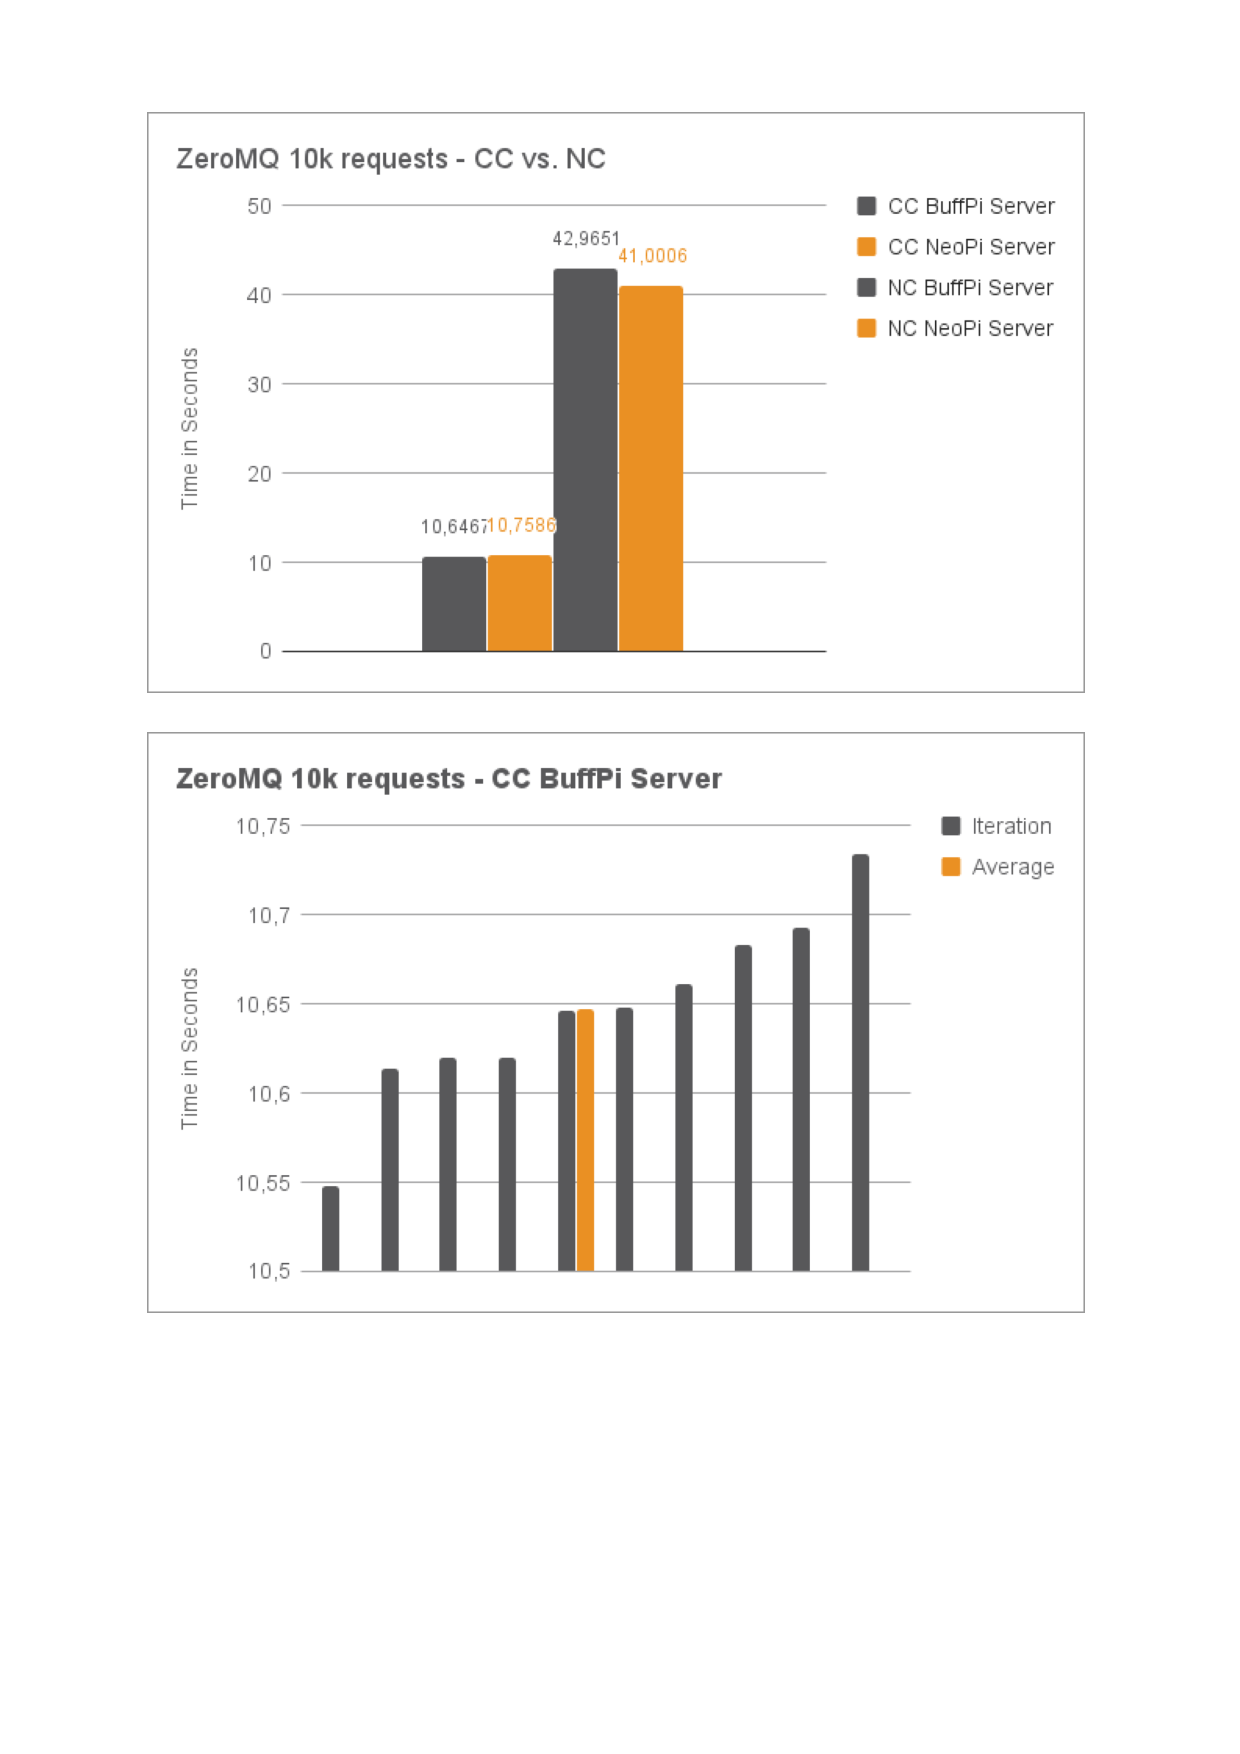
\includepdf[pages=-]{resources/pdfs/MA_Testergebnisse_-_ZeroMQ_Graphs.pdf}



\pagenumbering{Roman}
\setcounter{page}{1}

\cleardoublepage
\renewcommand*{\chapterthumbformat}{Acronyms}
\phantomsection
\addcontentsline{toc}{chapter}{Acronyms}
\renewcommand\refname{Acronyms}
\section*{Acronyms}
\begin{acronym}[NFV-MANO] % längste Abkürzung steht in eckigen Klammern
    \setlength{\itemsep}{-\parsep} % geringerer Zeilenabstand

    % A
    \acro{AE}{Autoscaling Engine}
    \acro{AES}{Advanced Encryption Standard}
    \acro{AMQP}{Advanced Message Queuing Protocol}
    \acro{API}{Application Programming Interface}
    % B
    \acro{BSS}{Business Support Systems}
    % C
    \acro{CapEx}{Capital Expenditure}
    \acro{CDN}{Content Delivery Network}
    \acro{CI}{Continuous Integration}
    \acro{CLI}{Command Line Interface}
    \acro{CORS}{Cross-Origin Resource Sharing}
    \acro{CPU}{Central Processing Unit}
    \acro{CPS}{Cyber-Physical System}
      \acroplural{CPS}[CPSs]{Cyber-Physical Systems}
    \acro{CSRF}{Cross-Site Request Forgery}
    \acro{CS}{Cyber System}
    \acro{CSS}{Cascading Style Sheets}
    % D
    \acro{DI}{Dependency Injection}
    % E
    \acro{EPGM}{Encapsulated Pragmatic General Multicast}
    \acro{EMS}{Element Management System}
    \acro{ETSI}{European Telecommunications Standards Institute}
    % F
    \acro{FM}{Fault Management}
    \acro{FOKUS}{Fraunhofer-Institut für Offene Kommunikationssysteme}
    % G
    \acro{GUI}{Graphical User Interface}
    % H
    \acro{H2H}{Human-to-Human}
    \acro{H2M}{Human-to-Machine}
    \acro{HATEOAS}{Hypermedia As The Engine Of Application State}
    \acro{HTML}{Hypertext Markup Language}
    \acro{HTTP}{Hypertext Transfer Protocol}
    % I
    \acro{IDE}{Integrated Development Environment}
      \acroplural{IDE}[IDEs]{Integrated Development Environments}
    \acro{IERC}{European Research Cluster on the Internet of Things}
    \acro{IoC}{Inversion of Control}
    \acro{IoE}{Internet of Energy}
    \acro{IoP}{Internet of People}
    \acro{IoS}{Internet of Services}
    \acro{IoT}{Internet of Things}
    \acro{IIoT}{Industrial Internet of Things}
    \acro{IP}{Internet Protocol}
    \acro{IPC}{Inter-Process Communication}
    \acro{IT}{Information Technology}
    % J
    \acro{JSON}{JavaScript Object Notation}
    \acro{JVM}{Java Virtual Machine}
    % K
    % L
    \acro{LXC}{Linux Containers}
    % M
    \acro{M2M}{Machine-to-Machine}
    \acro{MANO}{Management And Orchestration}
    \acro{MQTT}{Message Queue Telemetry Transport}
    % N
    \acro{NF}{Network Function}
      \acroplural{NF}[NFs]{Network Functions}
    \acro{NFV}{Network Function Virtualistion}
    \acro{NFVI}{Network Function Virtualization Infrastructure}
    \acro{NFV-MANO}{Network Function Virtualistion Management And Orchestration}
    \acro{NFVO}{Network Function Virtualistion Orchestrator}
    \acro{NIST}{National Institute of Standards and Technology}
    % O
    \acro{OASIS}{Organization for the Advancement of Structured Information Standards}
    \acro{OpEx}{Operating Expense}
    \acro{OS}{Operating System}
      \acroplural{OS}[OSs]{Operating Systems}
    \acro{OSS}{Operations Support Systems}
    % P
    \acro{PGM}{Pragmatic General Multicast}
    \acro{PNF}{Physical Network Function}
    \acro{PoP}{Point of Presence}
      \acroplural{PoP}[PoPs]{Points of Presence}
    % Q
    \acro{QoS}{Quality of Service}
    % R
    \acro{RAM}{Random Access Memory}
    \acro{REST}{Representational State Transfer}
    \acro{RFID}{Radio Frequency Identification}
    % S
    \acro{SDK}{Software Development Kit}
    \acro{SDN}{Software Defined Networking}
    \acro{SSL}{Secure Sockets Layer}
    % T
    \acro{TCP}{Transmission Control Protocol}
    \acro{TLS}{Transport Layer Security}
    \acro{TOSCA}{Topology and Orchestration Specification for Cloud Applications}
    % U
    \acro{UI}{User Interface}
    \acro{URL}{Uniform Resource Locator}
    % V
    \acro{VAL}{Virtualization Abstraction Layer}
    \acro{VIM}{Virtual Infrastructure Manager}
      \acroplural{VIM}[VIMs]{Virtual Infrastructure Managers}
    \acro{VM}{Virtual Machine}
      \acroplural{VM}[VMs]{Virtual Machines}
    \acro{VMM}{Virtual Machine Monitor}
    \acro{VNF}{Virtual Network Function}
      \acroplural{VNF}[VNFs]{Virtual Network Functions}
    \acro{VNFM}{Virtual Network Function Manager}
    % W
    % X
    % Y
    \acro{YAML}{YAML Ain\'t Markup Language}
    % Z
\end{acronym}


\cleardoublepage
\renewcommand*{\chapterthumbformat}{Glossary}
\phantomsection
\addcontentsline{toc}{chapter}{Glossary}
\renewcommand\refname{Glossary}
\section*{Glossary}

\interlinepenalty=10000 % keine Schusterjungen, keine Hurenkinder



\begin{description}

  \item[\bf{Algorithmus}] a

  \item[\bf{Chiffrierung}] a

  \item[\bf{Dechiffrierung}] a

\end{description}
\interlinepenalty=100


%\nocite{*} % auch die nicht verwendeten bibtex-Einträge einblenden
\cleardoublepage
\renewcommand*{\chapterthumbformat}{Bibliography}
\addcontentsline{toc}{chapter}{Bibliography}
\bibliography{bib/bibliography}
\interlinepenalty=100

%% Schmutzblatt (leere Seite am Ende)
\newpage
\pagestyle{empty}
\begin{figure}[H]
\centering

\includegraphics[width=0.9\textwidth]{resources/images/leer.jpg}
\end{figure}

\mtcaddchapter

\include{sections/xx4_index}

\end{document}
